\chapter{Self-Clocked Round-Robin Packet Scheduling for Better Burst Control} \label{chap:chap-3}


% epigraph after chapter heading
% \epigraph{The unavoidable price of reliability is simplicity.}{-- C. A. R. Hoare}


%%%% MUST: add the citation for the chapter if it is a reprint


\section{Packet Scheduling for Modern Internet}
\label{sec:scrr-background}

% Deficit Round Robin \cite{drr} has emerged as one of the best compromise among packet schedulers, due to its fairness, low complexity and its compatibility with any transport and any traffic. We argue that Deficit Round Robin is no longer suited for the mixed Internet workloads that consist of heavy, throughput-intensive flows, as well as bursty latency-sensitive flows.
Internet workloads incorporate a mix of heavy, throughput-intensive flows, as well as bursty latency-sensitive flows with diverse arrival patterns. Can Deficit Round Robin \cite{drr}, as the de facto candidate for fair scheduling cope with modern traffic characteristics?



\subsection{A Brief History of Packet Scheduling}
\label{sec:schedulers}

Historically, Packet-by-packet Generalized Processor Sharing (PGPS) \cite{gps} was among the first scheduling paradigms that target fair bandwidth allocation among tenants. Tenants or flows are classified into separate FIFO queues that are then processed by the packet scheduler. Subsequently, numerous Fair Queuing schedulers \cite{sparrow,scfq,stfq,frr,drr,mqfq,wfq} were introduced with distinct bounds and computational complexities. 
Classical Fair Queuing algorithms such as Start-Time Fair Queuing (STFQ) \cite{stfq} have the downside of expensive per-packet sorting operations as they need to constantly track and update the bandwidth allocation for each flow and choose the most eligible sub-queue, i.e., the sub-queue with the least progress. Further, computing requirement scales up with the number of sub-queues.

Deficit Round Robin (DRR) scheduling addresses this shortcoming by
allowing constant complexity dequeue operations irrespective of scale
\cite{drr}. Instead of maintaining a sorted data structure to keep
track of flow progress, it visits each sub-queue in a round-robin
fashion and allocates a fixed amount of bytes, called
\textit{quantum}, to each queue at each round. The part of the quantum
that is too small to send the next packet is accumulated as a deficit
for the queue.
Other variants of DRR, including Weighted Round-Robin (\textit{WRR}) and
Modified Deficit Round Robin (\textit{MDRR}) \cite{cisco} can operate on
a limited number of FIFO queues strictly reserved for different flow
priorities \cite{intel810}. These variants have a coarser fairness
granularity (per priority group, instead of per-flow) and need to be
configured with a deficit value that determines the amount of bytes
each priority group transmits on each pass.

Due to its constant computational complexity and low memory footprint,
\textit{DRR} is one of the most widely deployed packet schedulers in both
software and hardware \cite{drr,loom,cisco,juniper,tc,pifo,intel810,intel710}.
Even with the emergence of novel queuing abstractions such as \textit{PIFO}
\cite{pifo} and calendar queues \cite{calendar} that offer advanced
traffic classification and shaping, \textit{DRR} endures as a robust and widely
used option for flow scheduling, particularly in scenarios where
intricate packet classification is unnecessary
\cite{demi,netchannel,corundum,justitia,sch-fq} and standard TCP
support is required.\footnote{We later compare the performance of
state-of-the-art implementations of \textit{PIFO}, such as AIFO \cite{aifo} and
\textit{SP-PIFO} \cite{sppifo}, with \textit{DRR} in \S\ref{sec:scrr-evaluation}. Our results
suggest that \textit{AIFO} suffers from severe throughput loss at large RTTs,
while \textit{SP-PIFO} causes heavy packet re-ordering.}

\begin{figure*}[t]
 \centering
\begin{subfigure}[t]{.24\linewidth}
    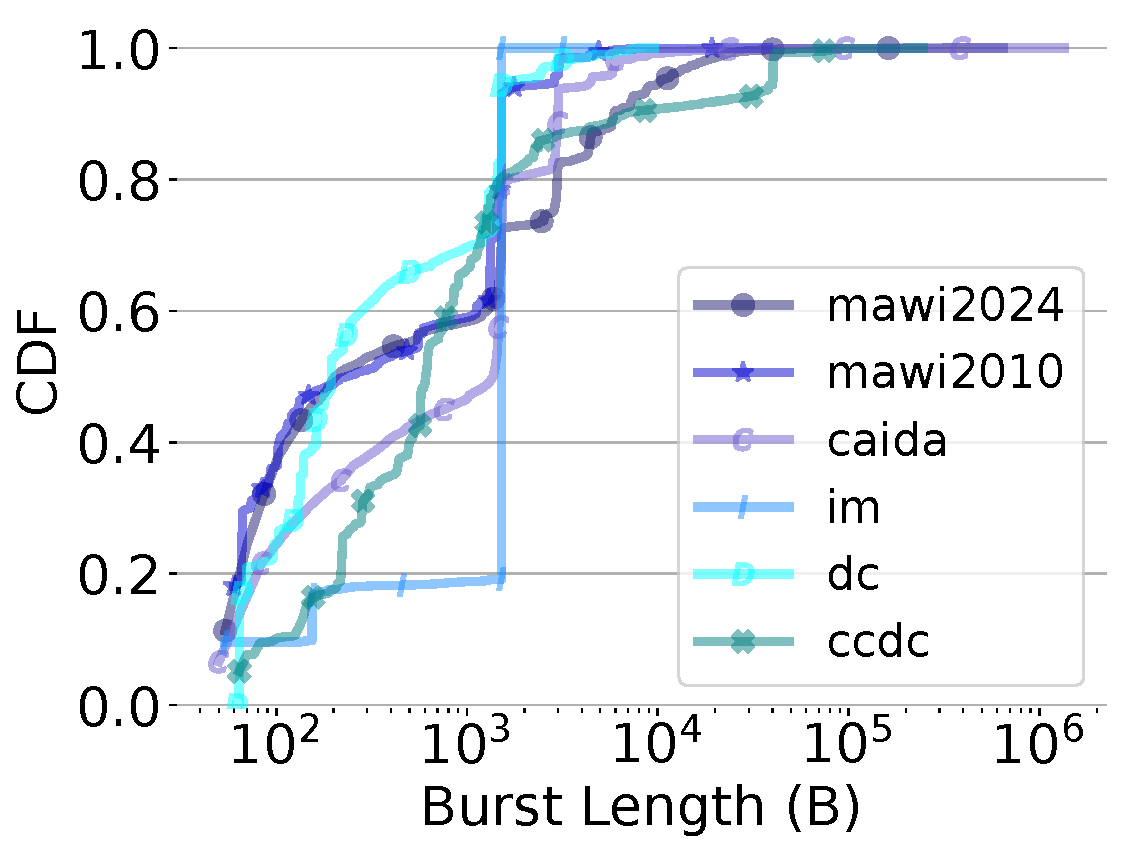
\includegraphics[width=\linewidth]{figs/aggregate_ipg_burstsize_cdf_10.pdf}
    \vspace{-6mm}
 \end{subfigure}
\begin{subfigure}[t]{.24\linewidth}
 \centering
    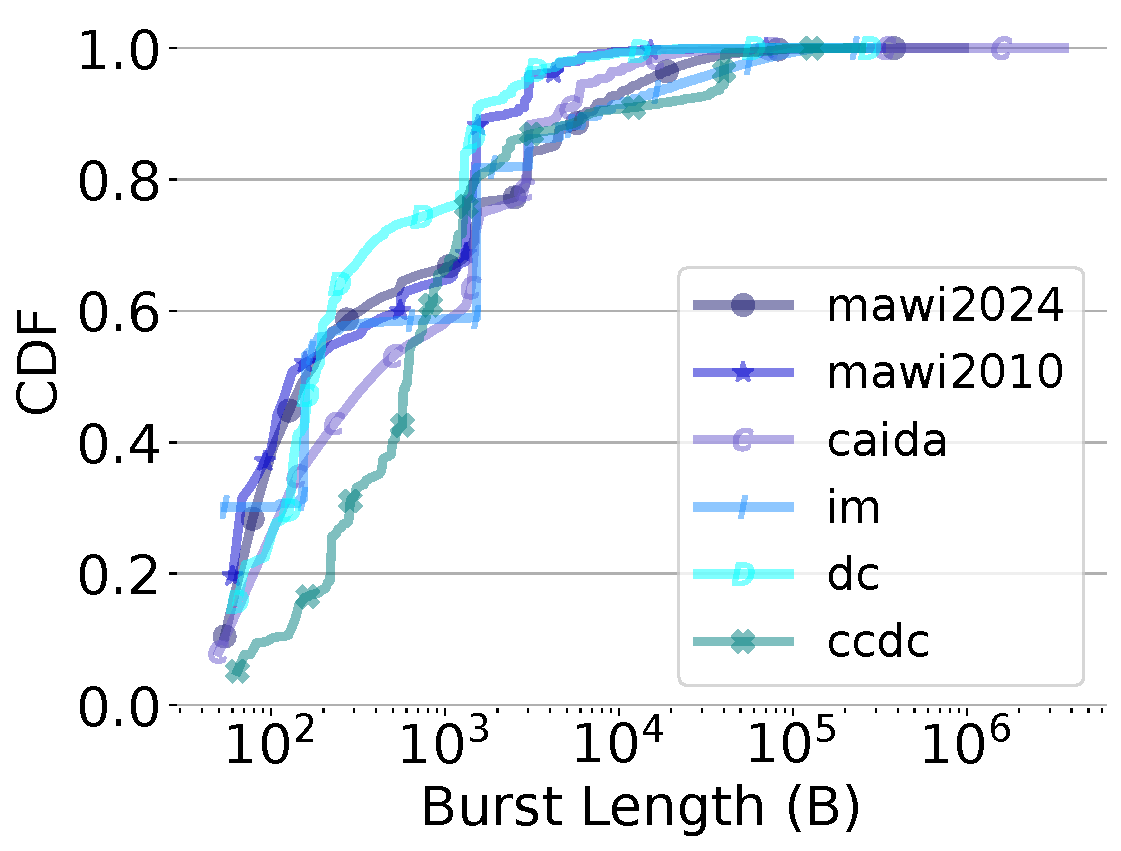
\includegraphics[width=\linewidth]{figs/aggregate_ipg_burstsize_cdf_50.pdf}
    \vspace{-6mm}
\end{subfigure}
\begin{subfigure}[t]{.24\linewidth}
 \centering
 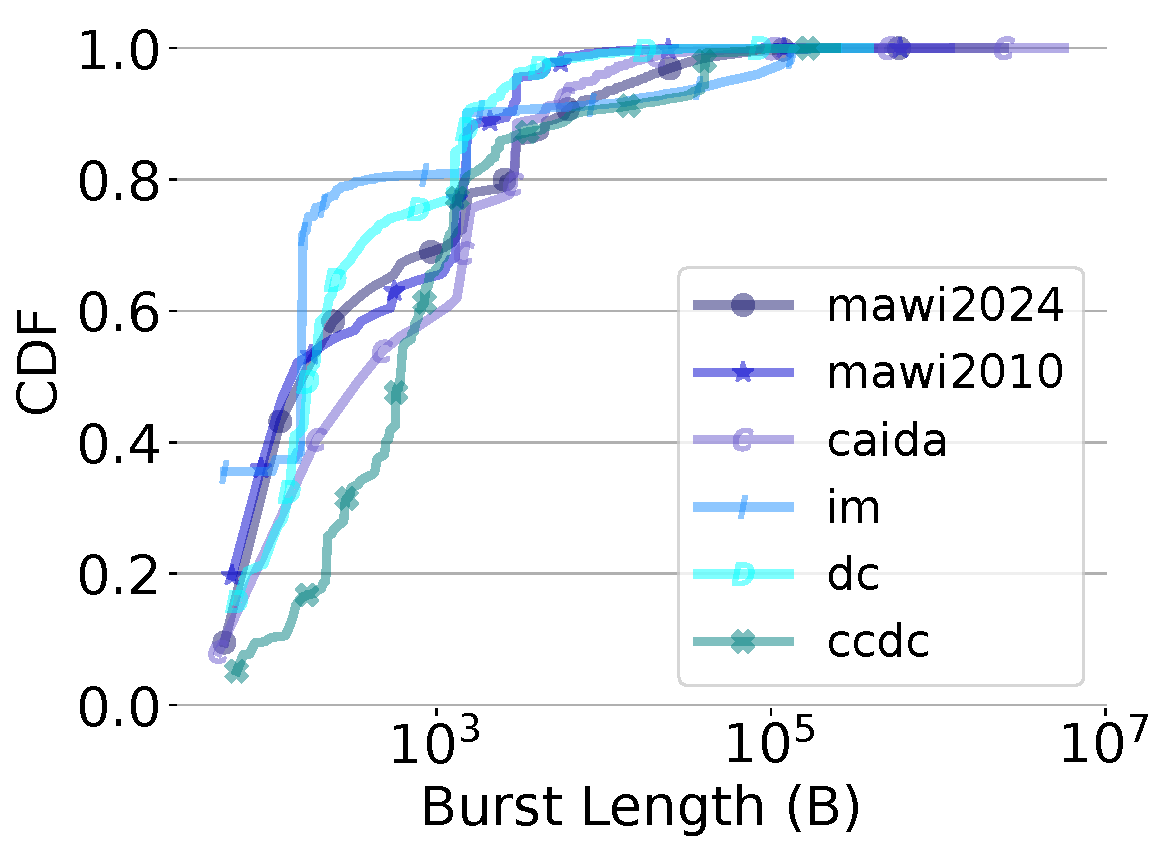
\includegraphics[width=\linewidth]{figs/aggregate_ipg_burstsize_cdf_100.pdf}
    \vspace{-7mm}
 \end{subfigure}
 \begin{subfigure}[t]{.24\linewidth}
 \centering
        \centering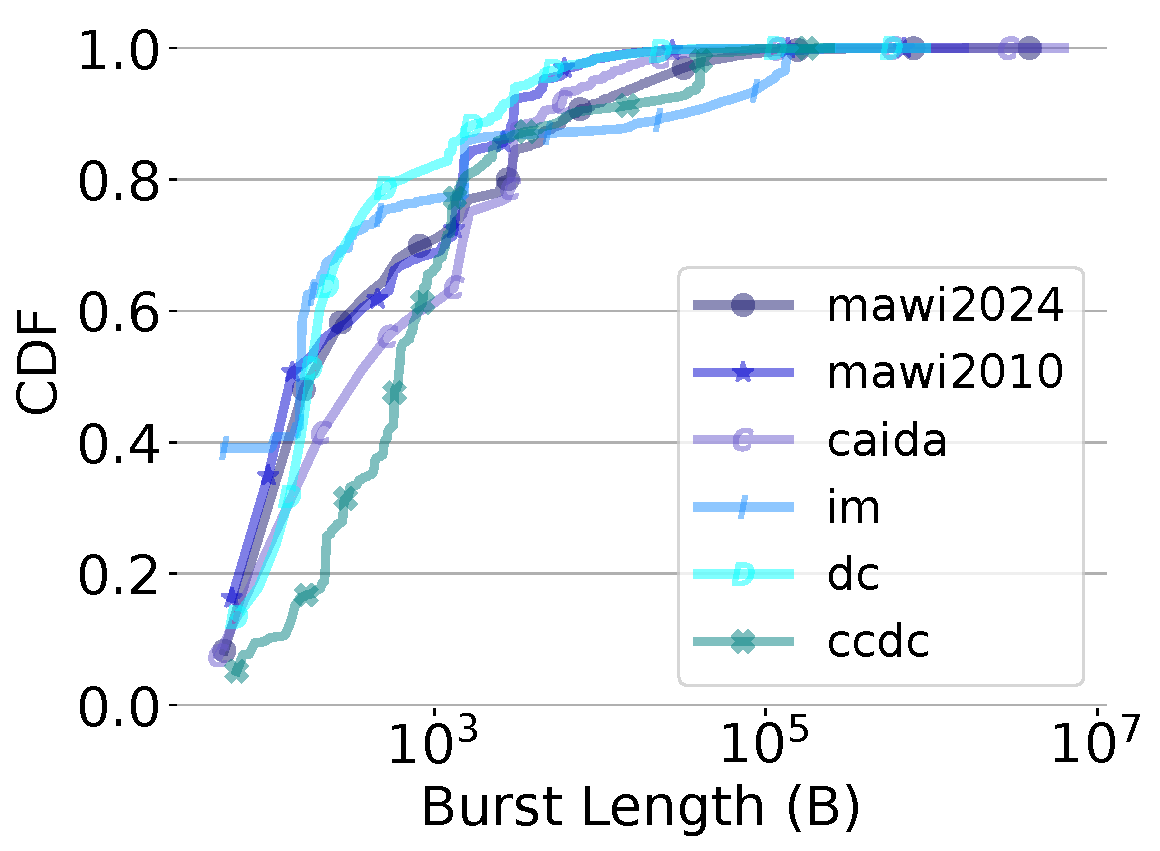
\includegraphics[width=1\linewidth]{figs/aggregate_ipg_burstsize_cdf_500.pdf}
         \vspace{-7mm}
\end{subfigure}
\begin{subfigure}[t]{.24\linewidth}
    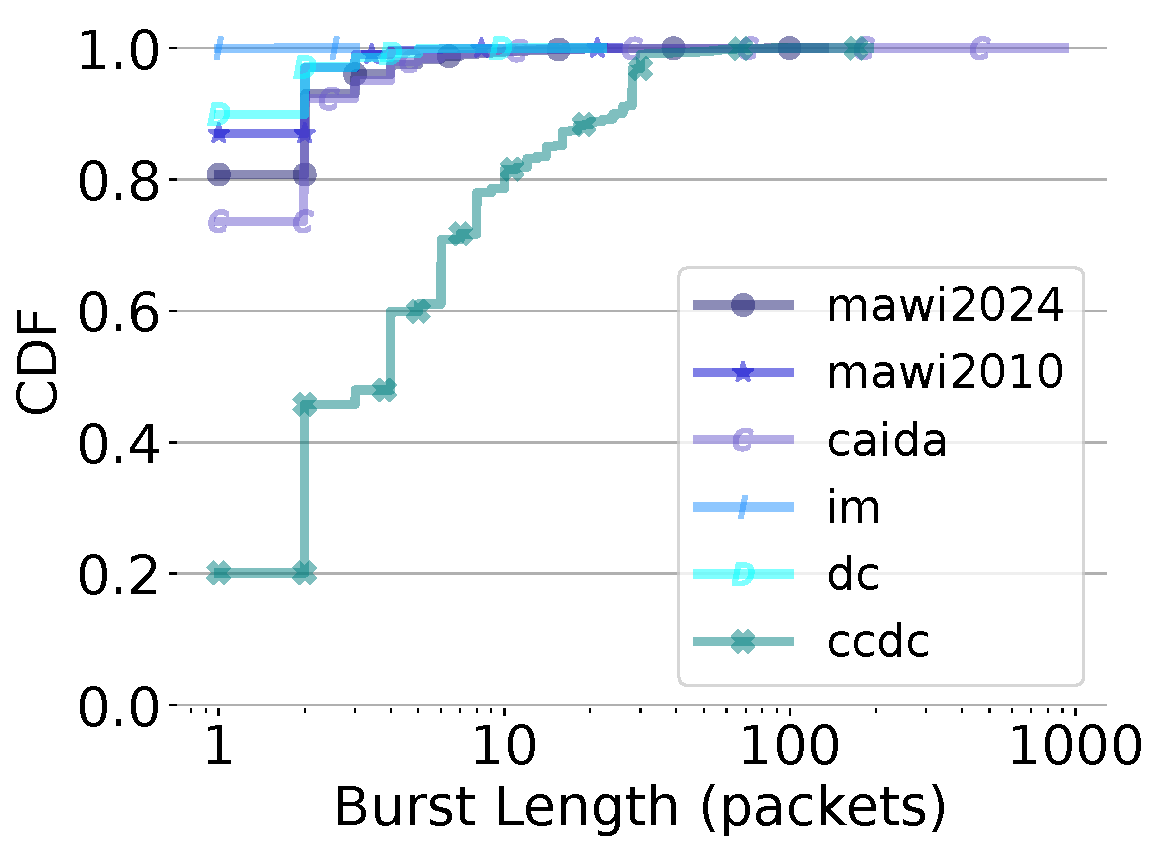
\includegraphics[width=\linewidth]{figs/aggregate_ipg_burstsize_pkt_cdf_10.pdf}
    \vspace{-6mm}
    \caption{\small{\textit{IPG < 10$\mu$s}}}
 \end{subfigure}
\begin{subfigure}[t]{.24\linewidth}
 \centering
    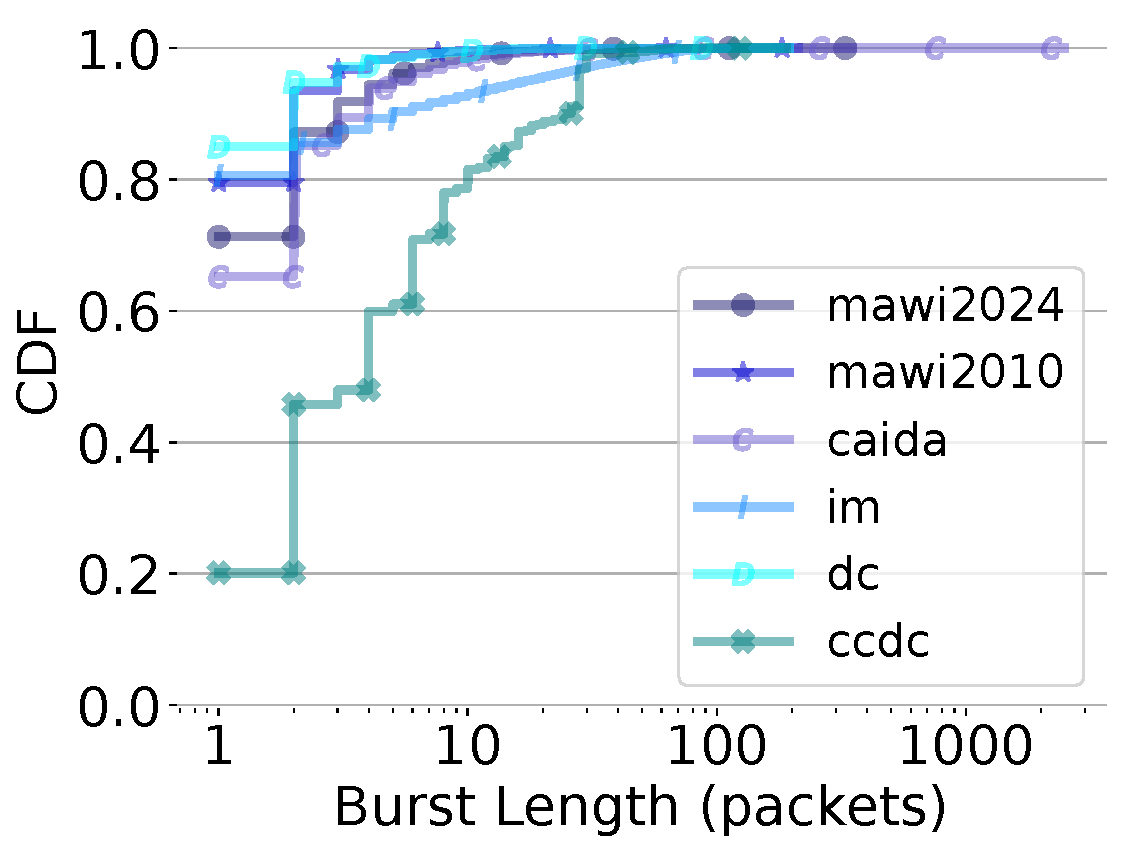
\includegraphics[width=\linewidth]{figs/aggregate_ipg_burstsize_pkt_cdf_50.pdf}
    \vspace{-6mm}
    \caption{\small{\textit{IPG < 50$\mu$s}}}
\end{subfigure}
\begin{subfigure}[t]{.24\linewidth}
 \centering
 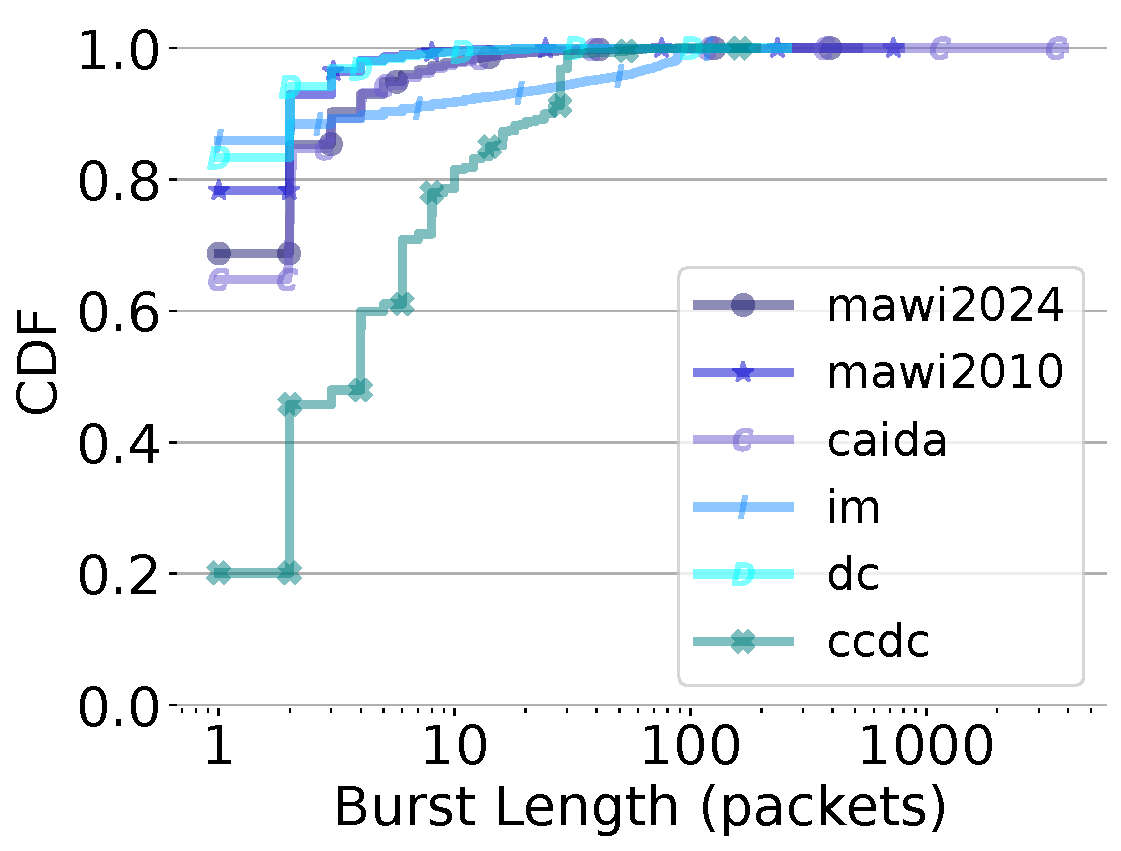
\includegraphics[width=\linewidth]{figs/aggregate_ipg_burstsize_pkt_cdf_100.pdf}
    \vspace{-6mm}
    \caption{\small{\textit{IPG < 100$\mu$s}}}
 \end{subfigure}
 \begin{subfigure}[t]{.24\linewidth}
 \centering
        \centering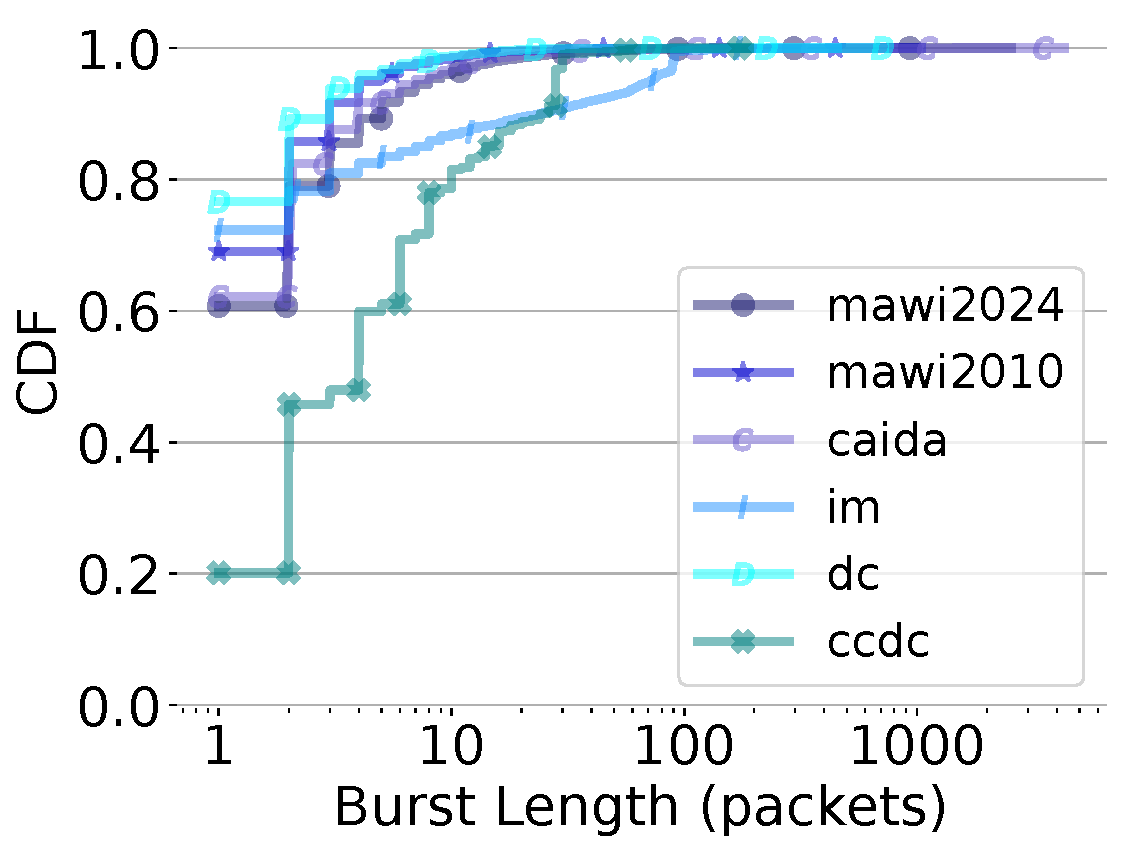
\includegraphics[width=1\linewidth]{figs/aggregate_ipg_burstsize_pkt_cdf_500.pdf}
         \vspace{-6mm}
		\caption{\small{\textit{IPG < 500$\mu$s}}}
\end{subfigure}
  \vspace{-0.3cm}
    \caption{\small{Burst length distribution for Internet traces using various IPG thresholds.}}
    \label{fig:traces-all}
  \vspace{-0.2cm}
\end{figure*}


\subsection{Flow Burstiness in Modern Traffic}

Burstiness is a well-known phenomenon for Internet traffic due to its multitude of root causes \cite{wild,bullet,why,im,valinor,high-resolution}. The emergence of interactive applications such as cloud gaming, video streaming, and video conferencing further underscores a type of traffic that experiences long idle times due to user behavior, network congestion, and variable bit-rate enforcement by the application \cite{im,movidiff,passive,qoe,gaming}. Traffic studies further report that many latency-sensitive workloads primarily produce short flows. For example, the median response size for web requests entering Facebook data centers is reported to be less than 10 kilobytes \cite{edge}, and frames in Zoom video traffic do not exceed 10 kB, with large gaps in between \cite{passive}. 
% The Inter-Packet Gap (IPG) distribution of Internet traces \cite{caida} in Fig \ref{fig:caida} further certify the existence of large gaps among packets of a flow.

A burst is a train of packets with inter-packet gaps smaller than a threshold \cite{bullet}. Using this definition, we plot the CDF of burst lengths for six representative Internet traces. These traces include backbone internet (\textit{caida}) \cite{caida} traces dating to 2019, campus network traces (\textit{dc}) \cite{wild}, ISP gateway traces for 2010 and 2024 (\textit{mawi}) \cite{mawi}, instant messaging (\textit{im}) \cite{im} packet traces and anonymized traces using in cyber defense competitions (\textit{ccdc}) \cite{ccdc}. According to Figure \ref{fig:traces-all}, regardless of the configured threshold, a diverse range of burst lengths can be observed which suggests that Internet workloads feature both heavily backlogged and short flows arriving at the bottlenecks. In fact. the similarity among burst size distributions with different IPG thresholds suggest that our analysis of Internet bursts is independent of the chosen threshold. Additionally,  the diversity in burst sizes suggests that not all Internet flows tend to remain active for a long time as they arrive at a bottleneck. Notably, many flows exhibit small bursts of packets followed by large idle periods. But we also see a number of very large bursts belonging to heavy flows likely to congest the packet scheduler.
Figure \ref{fig:trace-hurst} compares the hurst estimate (\S\ref{sec:valinor-background}) for the above traces. As previous studies point \cite{high-resolution}, network traffic is bursty and unpredictable for the most part. A small portion of traffic exhibits a strong self-similarity which suggests persistent burstiness at different timescales. These flows usually create backlogged queues on a fair packet scheduler. On the other hand many of the flows are composed of short bursts that can arrive at any time.

% \begin{figure*}[t]
%      \begin{minipage}[t]{0.21\textwidth}
%    	 \centering
%     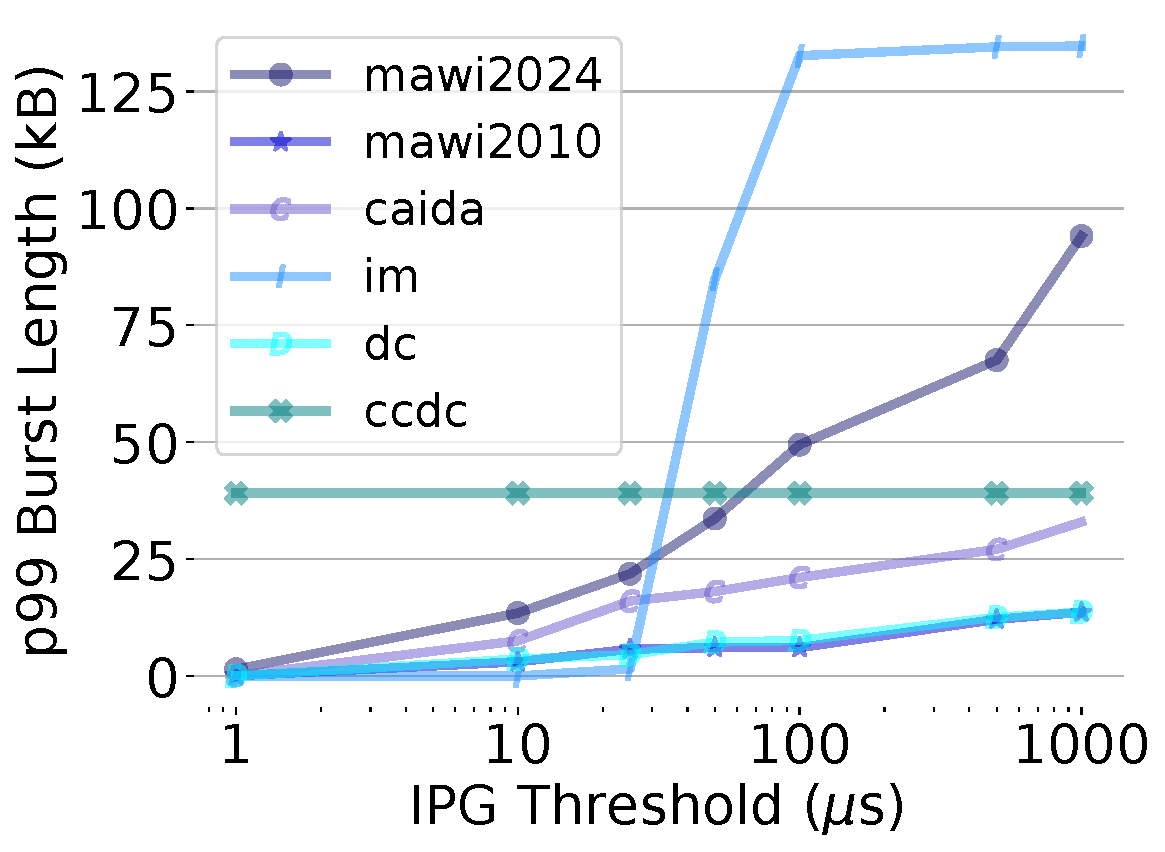
\includegraphics[width=\linewidth]{figs/aggregate_ipg_burstsize_p99.pdf}
%     \vspace{-6mm}
%     \caption{\small{\textit{p99 of burst sizes with different IPG thresholds shows various levels of burstiness. \todo{a 4 by two figure grid}}}}
% 	\label{fig:bursts-wild}
%   \end{minipage}
%        \hfill
%          \begin{minipage}[t]{0.18\textwidth}
%    	 \centering
%     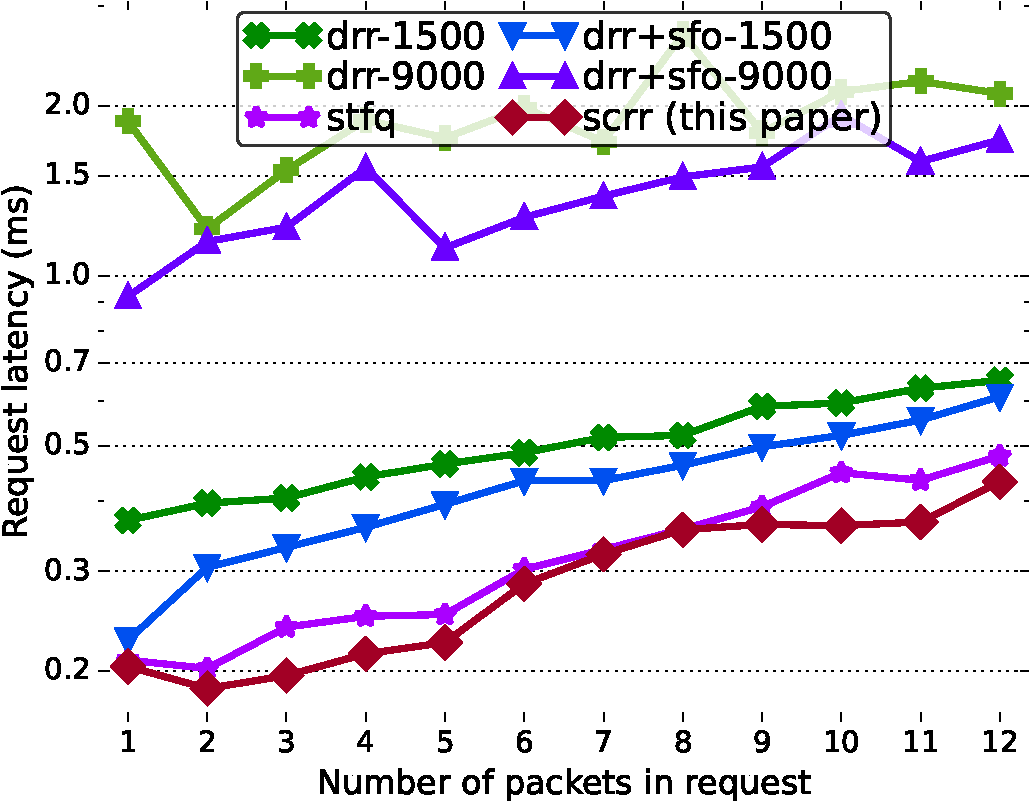
\includegraphics[width=\linewidth]{figs/pkt_num_lat_cn_2t4x16_mn_2tb2x4_mss_150_bql_9k_comp.pdf}
%     \vspace{-6mm}
%     \caption{\small{\textit{DRR offers poor application performance under different burst sizes. \todo{a simplified version of the figure (170s)}}}}
% 	\label{fig:drr-burst-latency}
%   \end{minipage}
%   \hfill
%       \begin{minipage}[t]{0.20\textwidth}
%     \centering
%     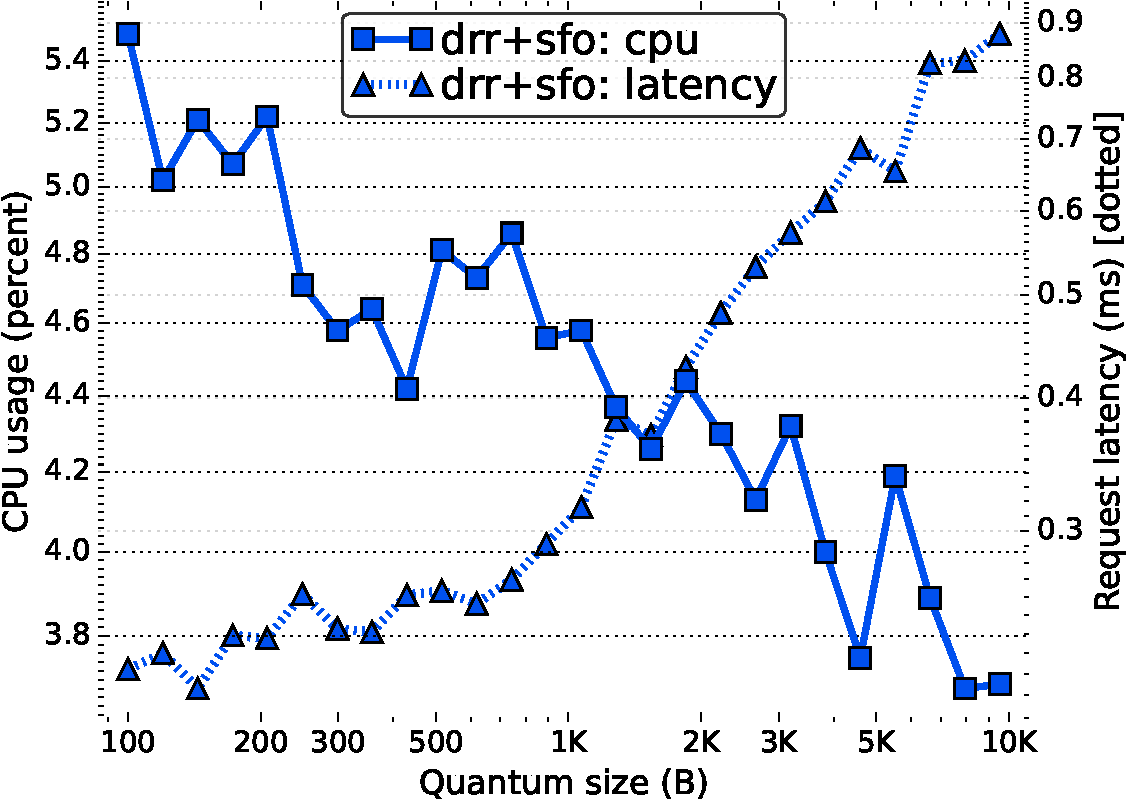
\includegraphics[width=1\linewidth]{figs/burst_cn_2t4x8_mn_2tb2x4_css_500_kp_lat_fq_drr.pdf}
%     \vspace{-6mm}
%     \caption{\small{\textit{Quantum in DRR trades-off CPU for better scheduling latency.}}}
% 	\label{fig:quanta-cpu-lat}
%   \end{minipage}
%   \hfill
%    \begin{minipage}[t]{0.19\textwidth}
%    		\centering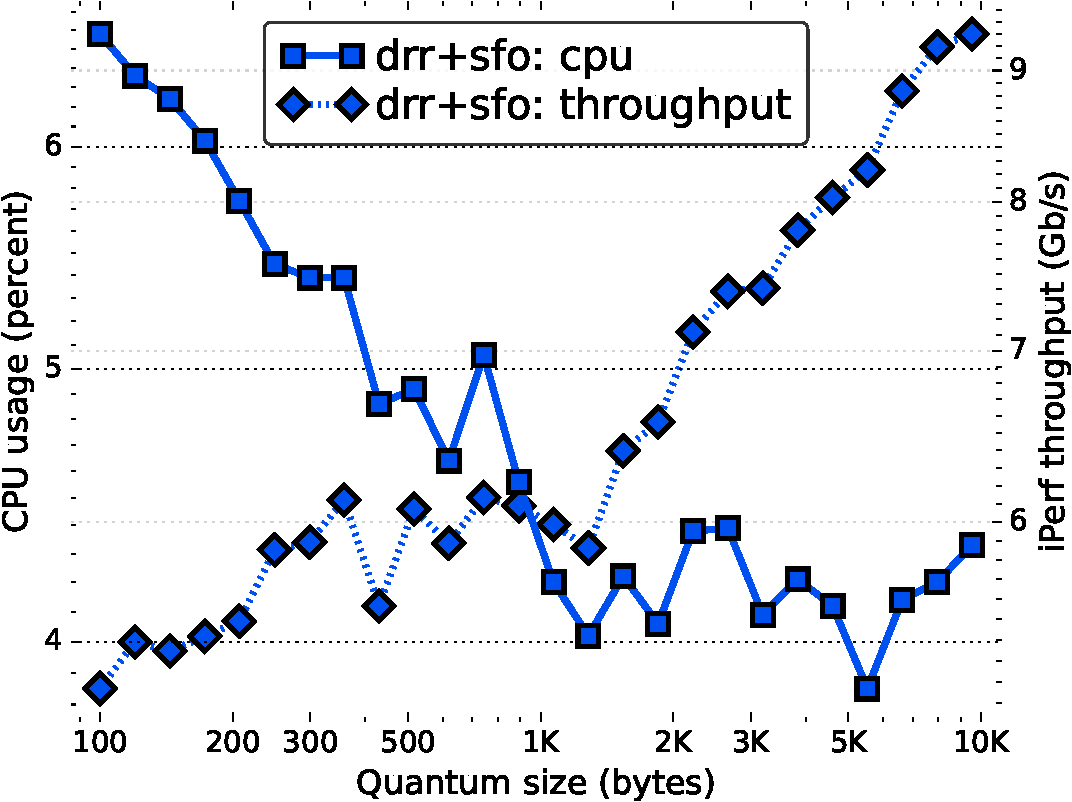
\includegraphics[width=1\linewidth]{figs/cpu_bandwidth.pdf}
%          \vspace{-6mm}
% 		\caption{\small{\textit{Increased CPU utilization quickly results in reduced bandwidth.}}}
%             \label{fig:cpu-bw}
%   \end{minipage}
%    \begin{minipage}[t]{0.19\textwidth}
%    		\centering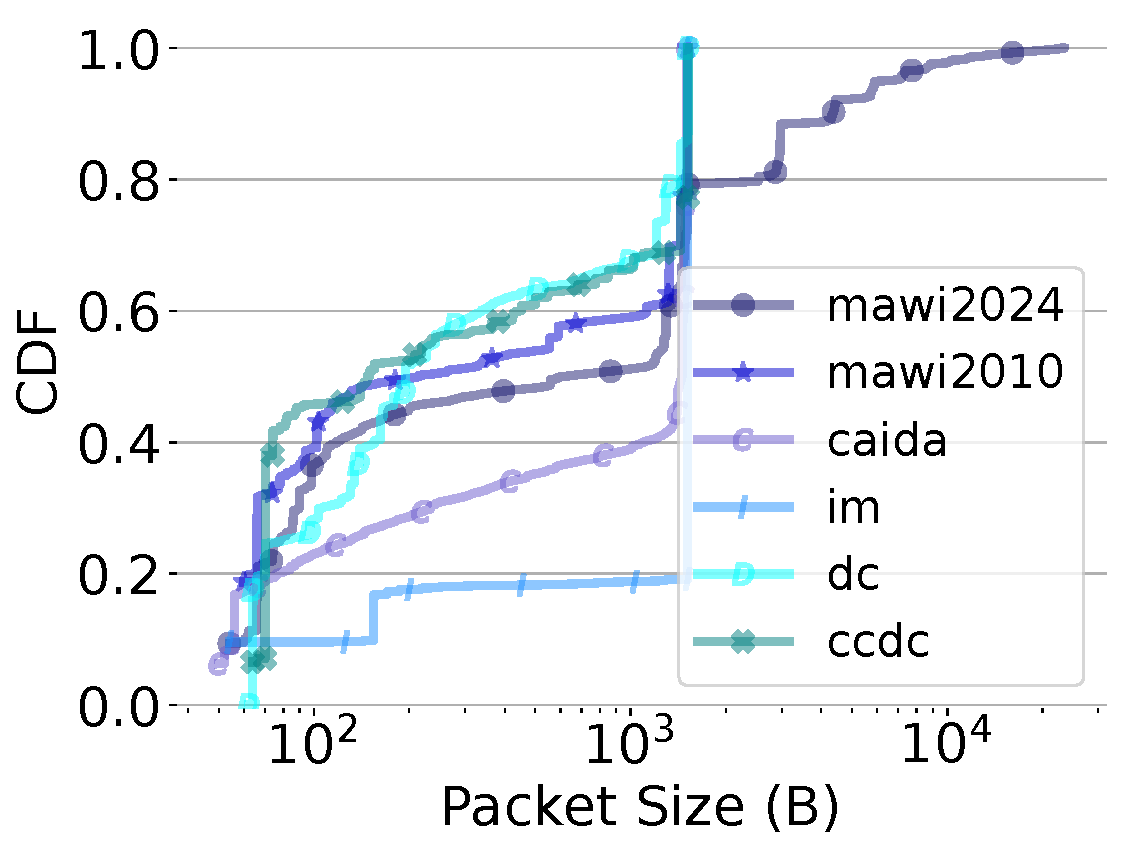
\includegraphics[width=1\linewidth]{figs/workload_dists.pdf}
%          \vspace{-6mm}
% 		\caption{\small{\textit{Packet length distributions in the wild is diverse and skewed.}}}
%             \label{fig:packets-wild}
%   \end{minipage}
%   \hfill
%   \vspace{-0.5cm}
% \end{figure*}

\begin{figure*}[t]

 \centering
  \begin{minipage}[t]{0.32\textwidth}
   	 \centering
    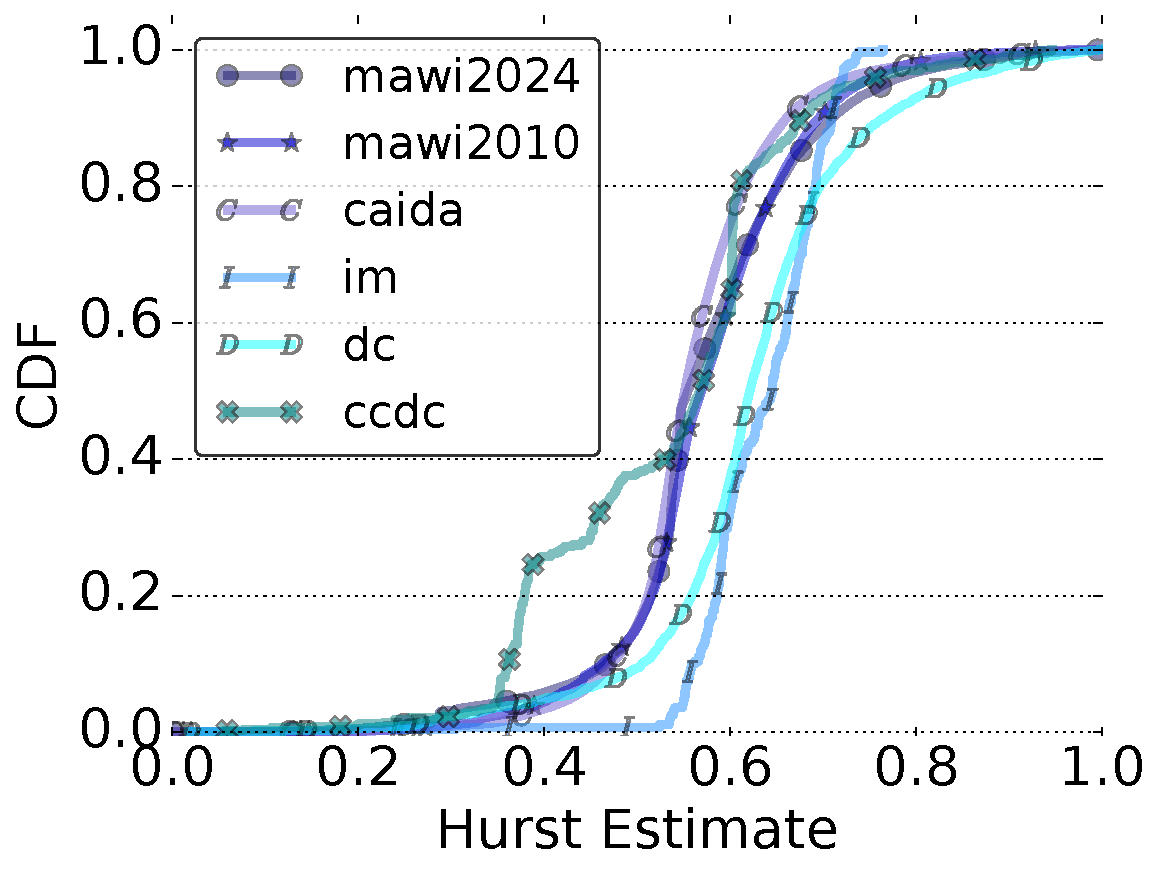
\includegraphics[width=\linewidth]{figs/hursts.pdf}
    \vspace{-7mm}
    \caption{\small{Hurst estimates for public packet traces.}}
	\label{fig:trace-hurst}
  \end{minipage}
  \begin{minipage}[t]{0.32\textwidth}
   	 \centering
    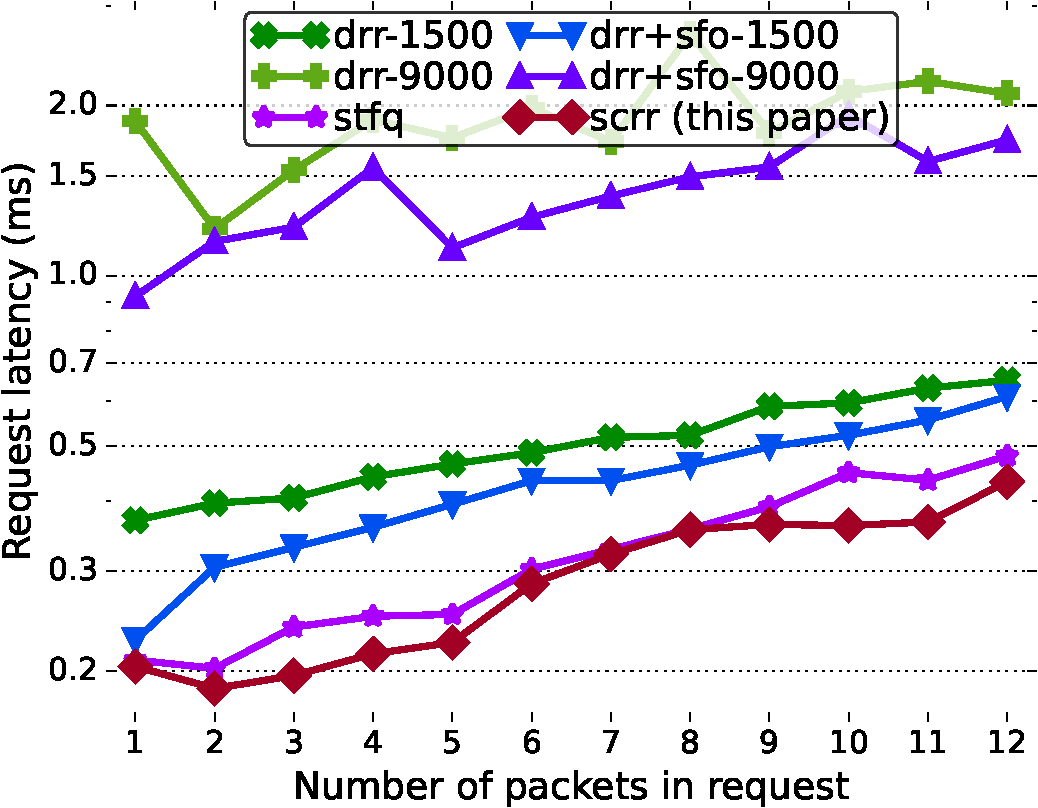
\includegraphics[width=\linewidth]{figs/pkt_num_lat_cn_2t4x16_mn_2tb2x4_mss_150_bql_9k_comp_fah.pdf}
    \vspace{-7mm}
    \caption{\small{DRR offers poor latency under different burst sizes.}}
	\label{fig:drr-burst-latency}
  \end{minipage}
  % \hfill
   \begin{minipage}[t]{0.32\textwidth}
     		\centering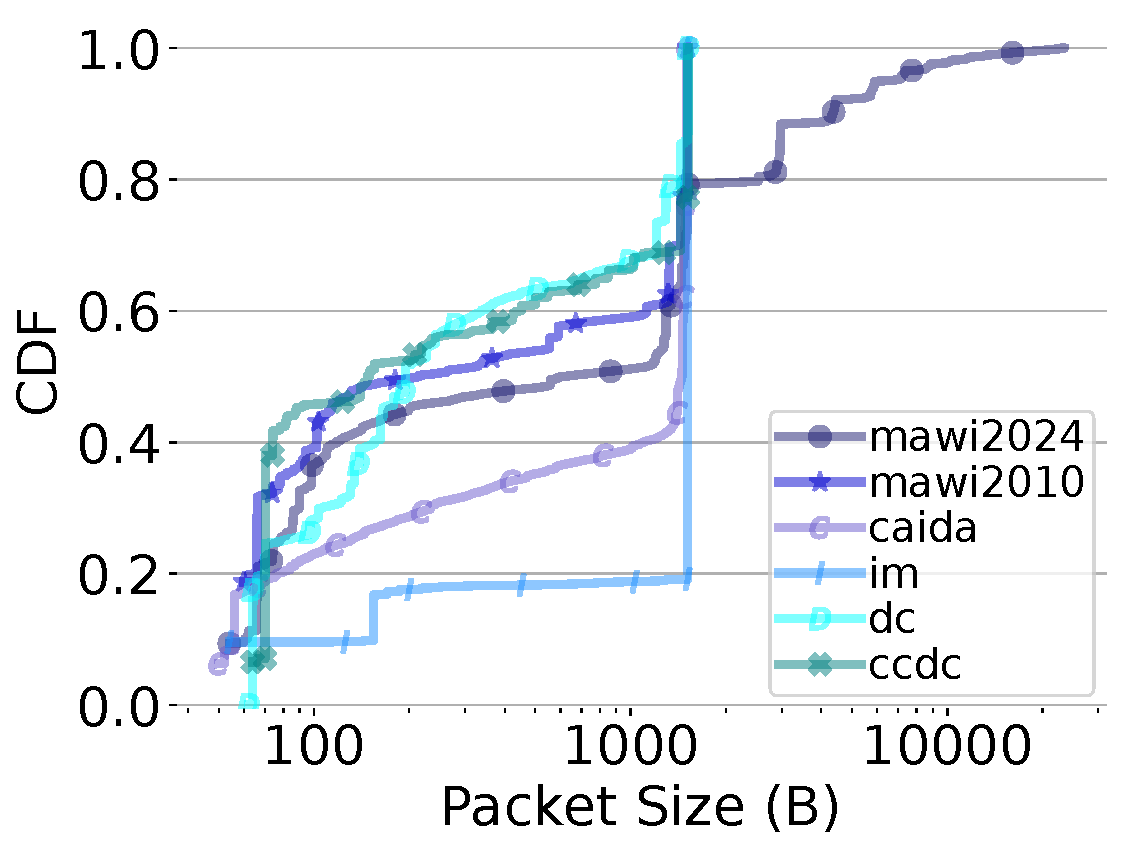
\includegraphics[width=1\linewidth]{figs/aggregate_ipg_pktsize_cdf.pdf}
         \vspace{-7mm}
		\caption{\small{Skewed packet length distributions in the wild.}}
            \label{fig:packets-wild}
  \end{minipage}
  \vspace{-0.2cm}
\end{figure*}
 


DRR has effectively the same theoretical bounds as Fair Queuing
schedulers (\S\ref{sec:schedulers}): it is fair and has a maximum
service deviation of 2$\times$ the quantum \cite {drr}. The fairness,
burstiness and latency guarantees of \textit{DRR} and Fair Queuing schedulers
are based on the assumption that all flows arriving at the scheduler
are always backlogged \cite{drr,scfq,stfq}. Alas, the above evidence
suggests that this is rarely the case for modern Internet traffic!
In practice, DRR usually has higher latency for those short bursty
flows which are not backlogged at the scheduler, and this is seldom
studied. With gaps in arrivals, short flows are prone to get stuck
behind backlogged flows in the scheduler.
Figure \ref{fig:drr-burst-latency} compares the response times for
a request-response workload under two software implementations of
\textit{DRR}, the original design presented in \cite{drr}, and the
state-of-the-art implementation of \textit{DRR} which implements \textit{Sparse
Flow Optimization (SFO)} \cite{sfo}, a technique that prioritizes
interactive traffic (\S\ref{sub:sfo}). We compare \textit{DRR} with two
different quantum settings: 1500B and 9000B, and with \textit{STFQ}
\cite{stfq}. Two senders generate a total of 16 parallel streams of requests
composed of bursts of 150B MSS packets, while the burst length increases on the x axis. Two other senders
generate 64 heavy flows each to ensure the scheduler is backlogged. The full
experiment setup can be found in \S\ref{sec:scrr-eval-latency}. Latency
gaps as large as 4$\times$ between \textit{DRR} and \textit{STFQ}
suggest that \textit{DRR} degrades the application performance due to
poor scheduling decisions regardless of its quantum setting, as
consecutive packets in a burst have to wait for full scheduling rounds
before they are transmitted. \textit{DRR+SFO} is initially able to
bridge this gap by boosting short flows through the scheduler, but as
the burst size increases, consecutive packets of the burst do not benefit from prioritization and have to wait.

%The implications of traffic behavior on packet scheduling warrant a closer study. Fair packet scheduling, often represented by DRR due to its practical implementation, mostly centers around strong fairness, low per-flow burstiness, low computation complexity, and high scalability for packet schedulers deployed in the wild. These characteristics are built based on the assumption that all flows arriving at the scheduler are always backlogged \cite{drr,scfq,stfq}. Alas, the above evidence suggests that this is rarely the case for modern Internet traffic! With gaps in arrivals, short flows are prone to get stuck behind backlogged flows in the scheduler. Fig. \ref{fig:drr-burst-latency} compares the response times for a request-response workload under two implementations of DRR, the original design presented in \cite{drr}, and the state-of-the-art implementation of DRR which separates new incoming flows from old active flows and gives strict priority to new flows in order to improve responsiveness. This mechanism is referred to as Sparse Flow Optimization (SFO) \cite{sfo}. We compare two different quantum settings: 1500B and 9000B with a software implementation of STFQ \cite{stfq} in a setup where we send a burst of 150B MSS packets as the request data. The full experiment setup can be found in \S\ref{evaluation}. The latency gaps as large as 4$\times$ between DRR and STFQ suggest that DRR degrades the application performance due to poor scheduling decisions regardless of its quantum setting as consecutive packets in a burst have to wait for full scheduling rounds before they are transmitted. DRR+SFO is initially able to bridge this gap by boosting short flows through the scheduler, but as the burst size increases, these flows are demoted to old flows and suffer from a similar fate as DRR.


% To demonstrate the impact of flow arrivals in the performance of packet scheduling, we run two separate latency-sensitive workloads, one using TCP cubic flows sending 500B request and response packets, while the other sends ICMP echo flows of similar size on the physical testbed described in \S\ref{sub:eval-gsogro}. The router node runs the original software implementation of DRR \cite{drr} that is also backlogged with 64 concurrent UDP flows that share the same bottleneck link as the latency-sensitive flows. Fig. \ref{fig:ping} presents the mean response times of latency-sensitive flows using lines and the 10th and 90th percentiles of their response times using error bars. Looking at the top lines, as we increase the quantum size for DRR, both workloads experience higher response times. For example, using a 9KB quantum for the backlogged scheduler increases the response times for both TCP and ICMP flows by around 3$\times$. This is because the latency-sensitive flows are delayed by background flows sending larger bursts of packets during their turn. 

% To account for this unwanted latency, recent works introduce \textit{Sparse Flow Optimization (SFO)} for the DRR scheduler by separating the list of new flows and old flows in the scheduler, with strict priority given to the flows that recently become active. SFO has made its way into Linux qdiscs that use DRR \cite{sfo}. We repeat our experiments with SFO and see surprising distinctions between the TCP and ICMP workloads. While the ICMP traffic detangles itself from DRR's quantum configuration, a large majority of TCP flows still experience degraded performance with increased quanta. This is because the gap between the acknowledgement packet and the response data packet is large enough that while the first packet is boosted through the new flows list, the response data packet will arrive after the flow is demoted to the old flows, so it has to wait for a full scheduling round to get serviced \cite{formal}. Unfortunately, resorting to a small quantum to avoid aggravated scheduling delays will violate DRR's theoretical bounds \cite{drr} and result in increased CPU utilization as we observe further in \S\ref{sec:drr-tradeoff}.

% The above findings hint at the presence of two flow categories: \textit{heavy} or \textit{sparse}.
% A \textit{heavy} flow can be identified by its tendency to always being active in the schedule due to having a packet waiting. Workloads such as file transfer and large downloads on the edge, proportions of web traffic, and machine learning and data mining transfers inside and between datacenters are a few examples \cite{deadline,codedbulk,bulk}. \textit{Sparse} flows can be defined as flows that do not use their fair share of bandwidth during a scheduling period, where the fair share is defined as the available capacity divided by (weighted) number of active flows during a period when all active flows are serviced. 
% Sparse flows are common in Internet traffic. Real-time communication application such as video conferencing, voice over IP, video and music streaming, and even web traffic commonly transmit in short bursts with long idle, reduced bit rate, or reduced packet length periods \cite{demistify,rfec,sparse}. 

% Looking at the literature on fair queueing, existing proposals fail to take both classes of flows into consideration. Apart from fair schedulers, there exits a large body of work in the data center domain that strongly advocate low latency using explicit flow classification from the end hosts \cite{afq,aifo,pifo,sppifo,calendar}.
% However, when targeting the general Internet, it is highly unrealistic to expect users to properly configure their packet scheduler to work under all workload patterns. On the other hand, the existing SFO mechanism suffers from two shortcomings. First, Separating the new and old flows creates non-deterministic loops and unnecessary visits to empty sub-queues, making the technique incompatible with hardware targets. Second, existing proposals assume DRR scheduling. As we stress throughout the paper, an improper setting of DRR's quantum can result in application performance degradation.



% Below, we define each property and present and compare the most notable fair queueing algorithms in the literature.
% Fairness is defined as the maximum deviation of service (service lag) between two flows during a fixed amount of time \cite{scfq}.
%, or more broadly the service proportion each flow receives after a sufficient amount of scheduling time \cite{drr}.
% Per-flow burstiness is defined as the maximum amount of bytes transmitted from each sub-queue on each scheduling pass. Lastly, computation complexity specifies the amount of compute resources required to run the scheduling algorithm as the scale of the workload (e.g., the number of active flows) increases. 
% This complexity contributes to the overall computation efficiency alongside implementation considerations such as cache efficiency.
% Similarly, memory complexity outlines the memory scalability of a scheduling algorithm. 

% \begin{figure*}[t]
  \centering
    \begin{minipage}[t]{0.48\textwidth}
    \begin{subfigure}[t]{.49\linewidth}
    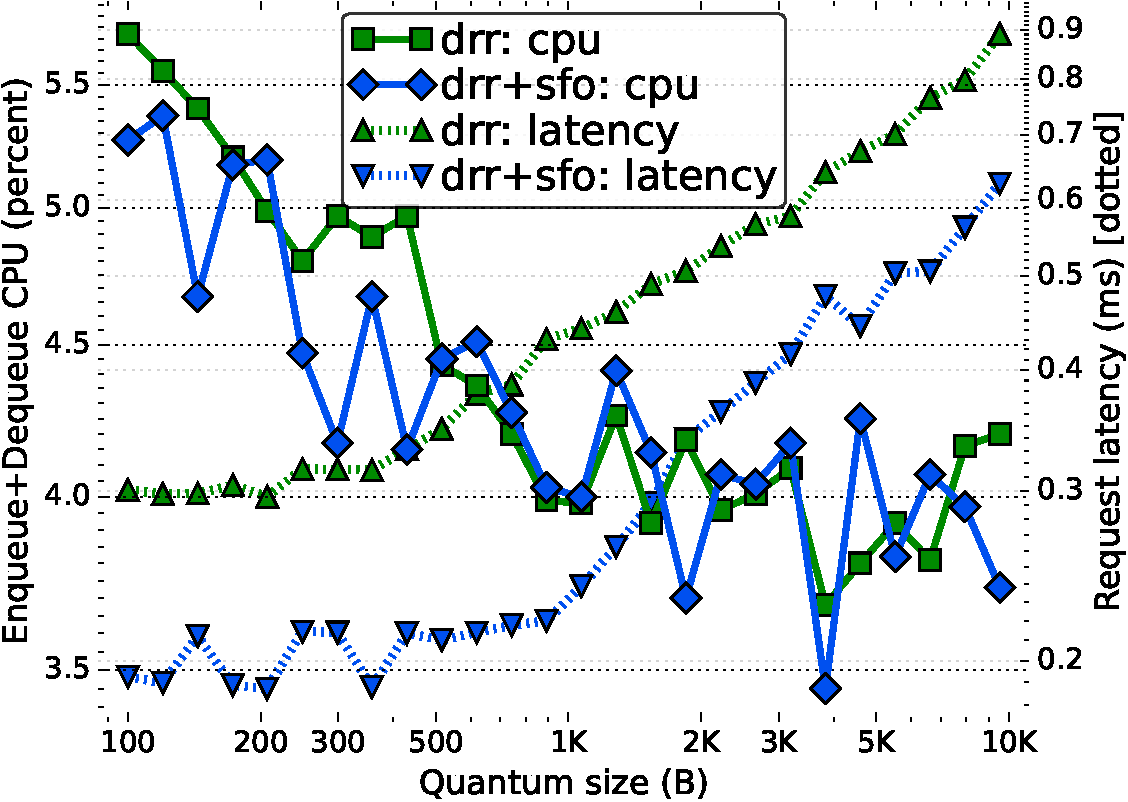
\includegraphics[width=1\linewidth]{figs/burst_cn_2t4x8_mn_2tb2x4_crs_500_kp_lat_drr_basic_fq_drr.pdf}
    \vspace{-6mm}
    \caption{\small{\textit{CPU vs scheduling latency}}}
	\label{fig:quanta-cpu-lat}
    \end{subfigure}
    \begin{subfigure}[t]{.49\linewidth}
        \centering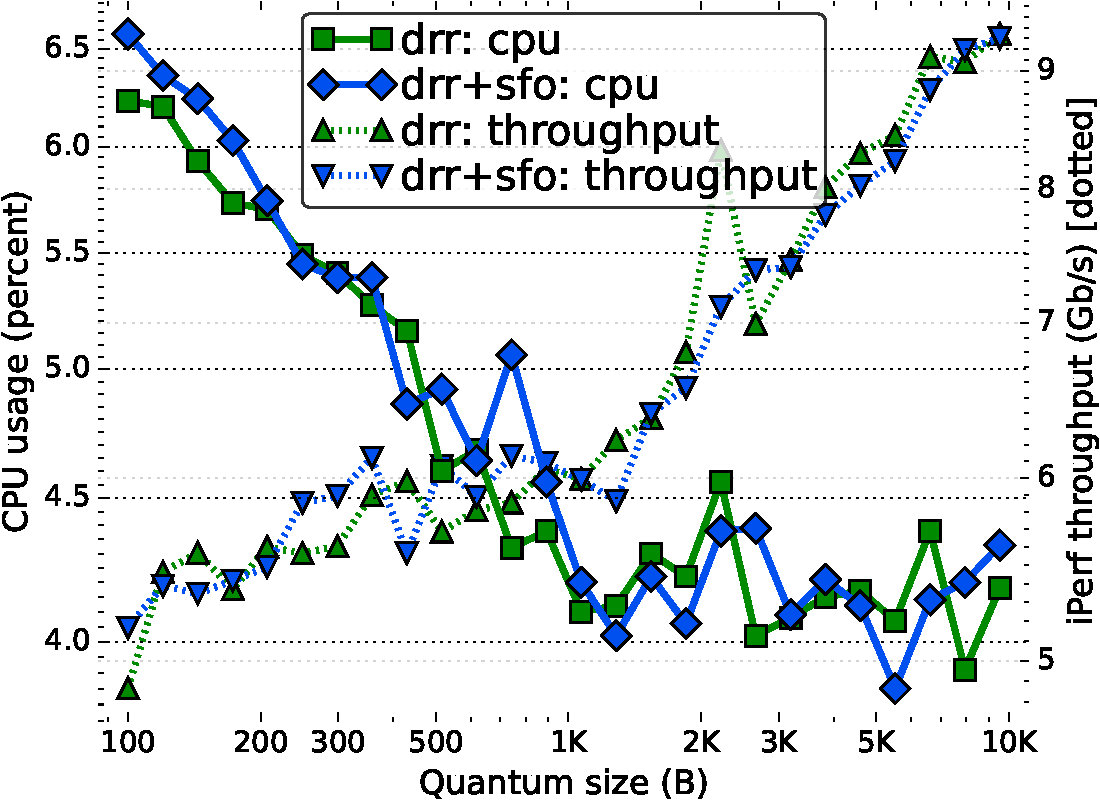
\includegraphics[width=1\linewidth]{figs/burst_cn_6t1x10_mss_1000_kp_bw_drr_basic_fq_drr.pdf}
         \vspace{-6mm}
		\caption{\small{\textit{CPU vs app. throughput}}}
            \label{fig:quanta-cpu-bw}
    \end{subfigure}
        \vspace{-2mm}
    	\caption{\small{
        \textit{Trade-offs in DRR's quantum configuration. }
		}}
	\label{fig:packets}
  \end{minipage}
        \begin{minipage}[t]{0.48\textwidth}
	\centering
	\begin{subfigure}[t]{.49\linewidth}
		\centering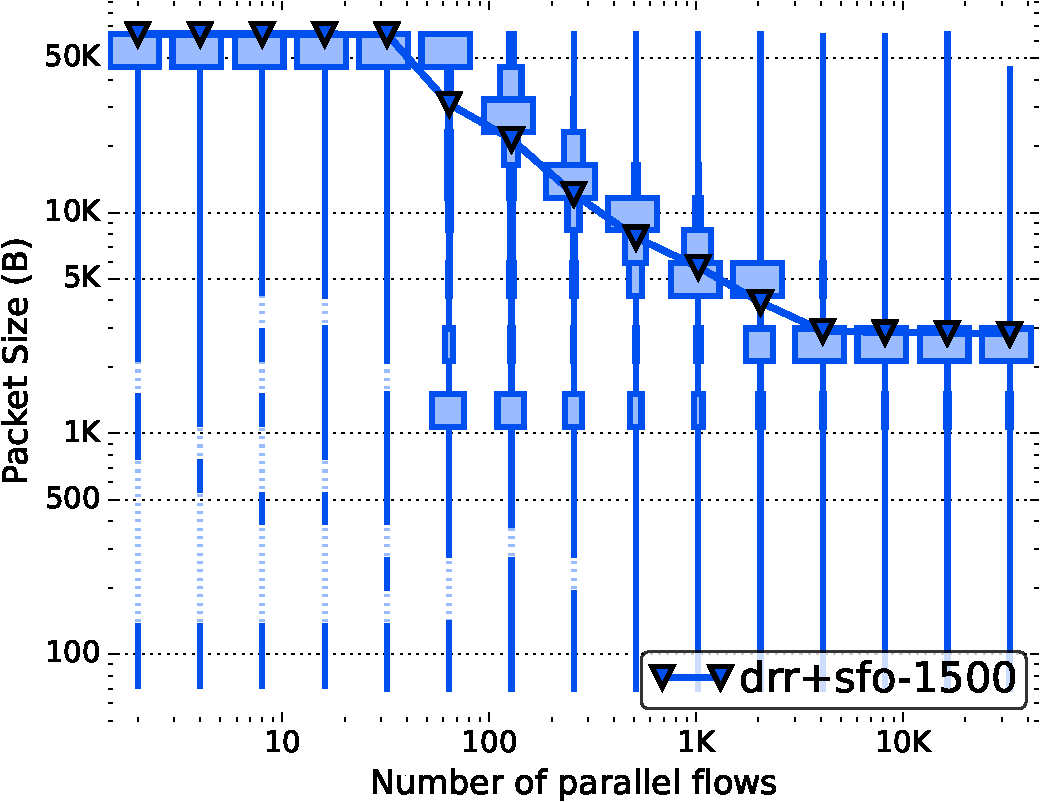
\includegraphics[width=1\linewidth]{figs/paral_cn_1t16x1024_gso_pkthist_fq_drr_1500.pdf}
  \vspace{-6mm}
		\caption{\small{\textit{TSO on TX machine}}}
            \label{fig:packets-edge}
	\end{subfigure}
	\begin{subfigure}[t]{.49\linewidth}
		\centering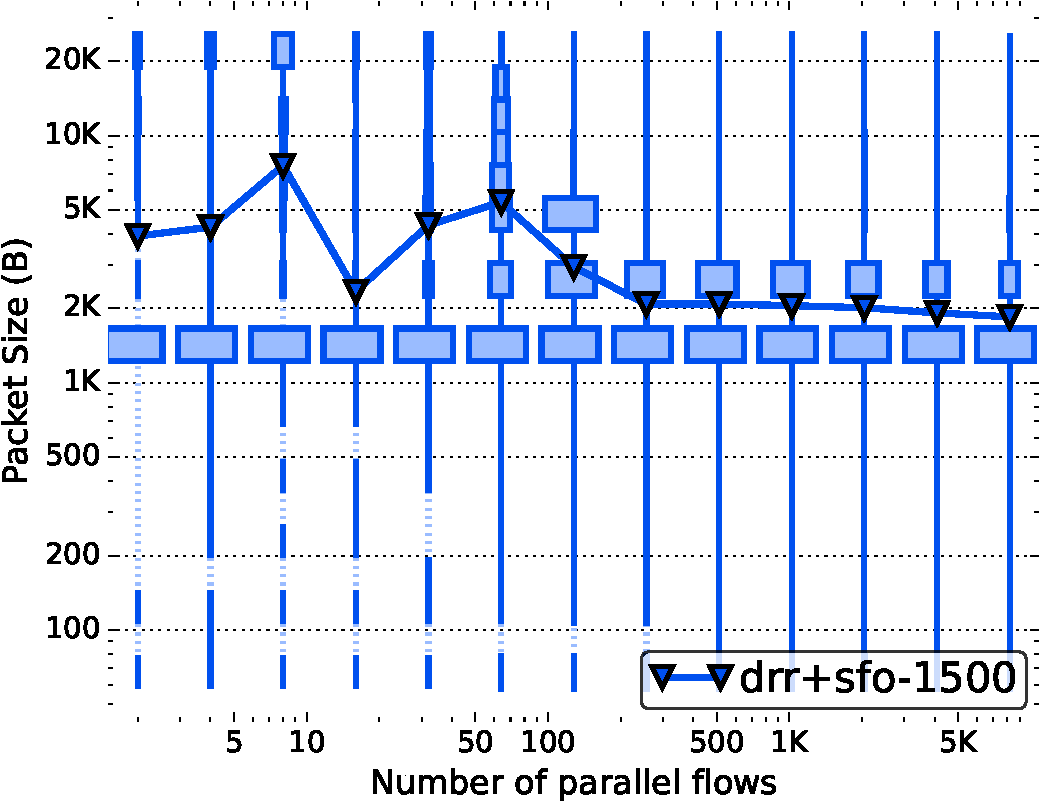
\includegraphics[width=1\linewidth]{figs/paral_cn_1t4x1024_gro_pkthist_fq_drr_1500.pdf}
  \vspace{-6mm}
		\caption{\small{\textit{LRO on RX machine}}}
            \label{fig:packets-core}
	\end{subfigure}
    \vspace{-2mm}
	\caption{\small{
        \textit{SKB length distribution under NIC offloading functions. }
		}}
	\label{fig:packets}
 \end{minipage}
  \vspace{-0.1cm}
\end{figure*}

% \begin{figure}[t]
% 	\centering
% 	\begin{subfigure}[t]{.49\linewidth}
% 		\centering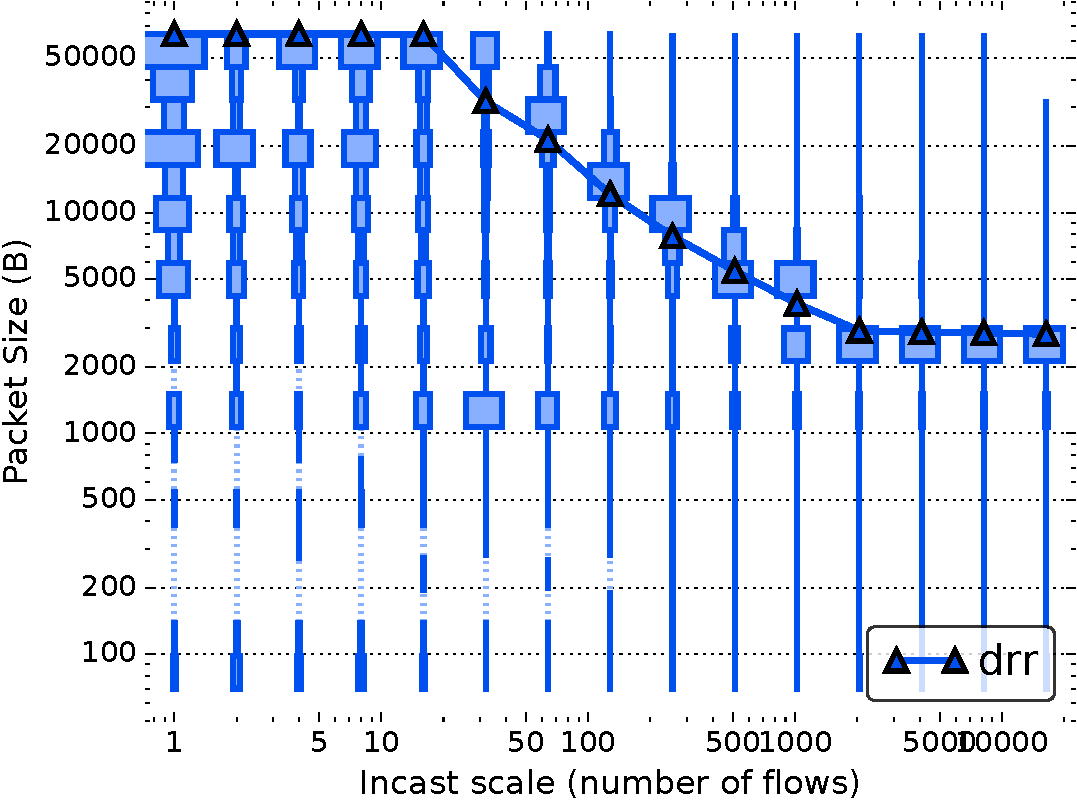
\includegraphics[width=1\linewidth]{figs/paral_pktlength_comp_methods_drr.pdf}
% 		\caption{TSO on TX machine}
%             \label{fig:packets-edge}
% 	\end{subfigure}
% 	\begin{subfigure}[t]{.49\linewidth}
% 		\centering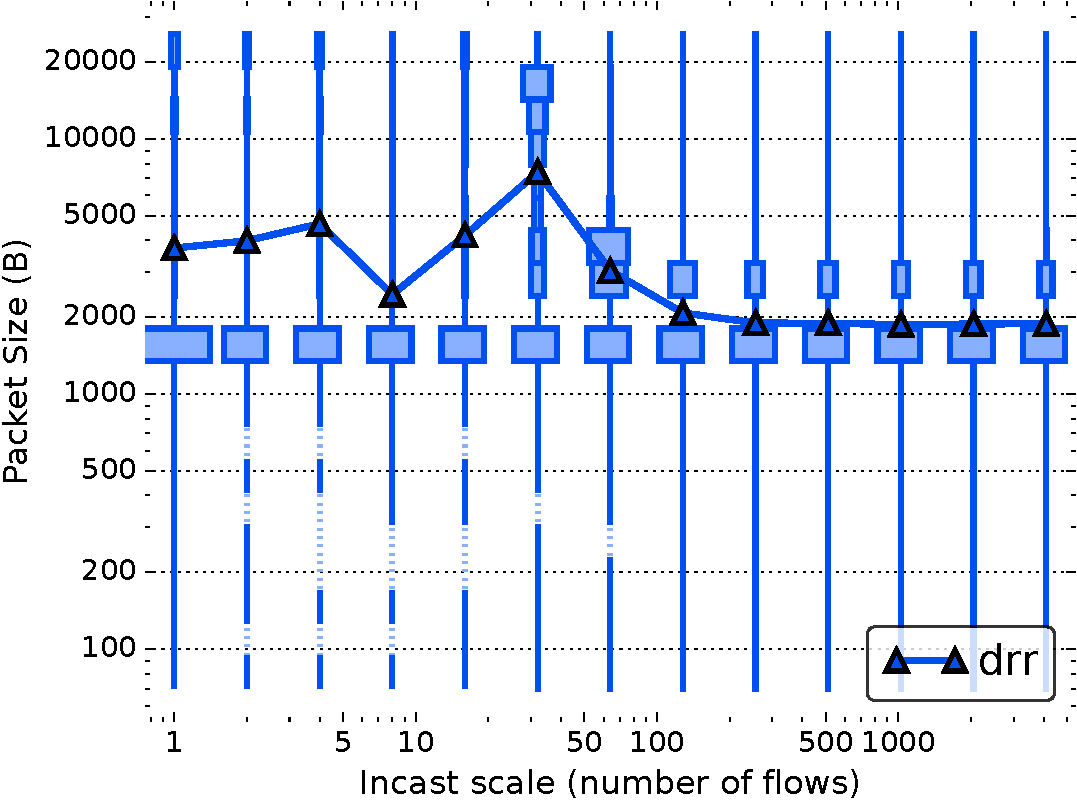
\includegraphics[width=1\linewidth]{figs/paral_pktlength_comp_methods_drr_lro.pdf}
% 		\caption{LRO on RX machine}
%             \label{fig:packets-core}
% 	\end{subfigure}
%     \vspace{-3mm}
% 	\caption{
%         Packet length distribution changes as the number of active TCP flows increases from 1 to 1024 for each connection pair. Enabling the TSO and LRO functionalities drastically widens the possible range of observed packet lengths. The distribution is represented via parallel, independent histogram charts. Wider bins demonstrate higher probability. The straight horizontal line presents the average packet length over different number of parallel flows.
% 		}
% 	\label{fig:packets}
% 	\vspace*{-0.7cm}

% 	\hspace{10pt}
% \end{figure}



% \begin{figure}[t]
    \centering
    \begin{subfigure}[t]{.40\linewidth}
        \centering
        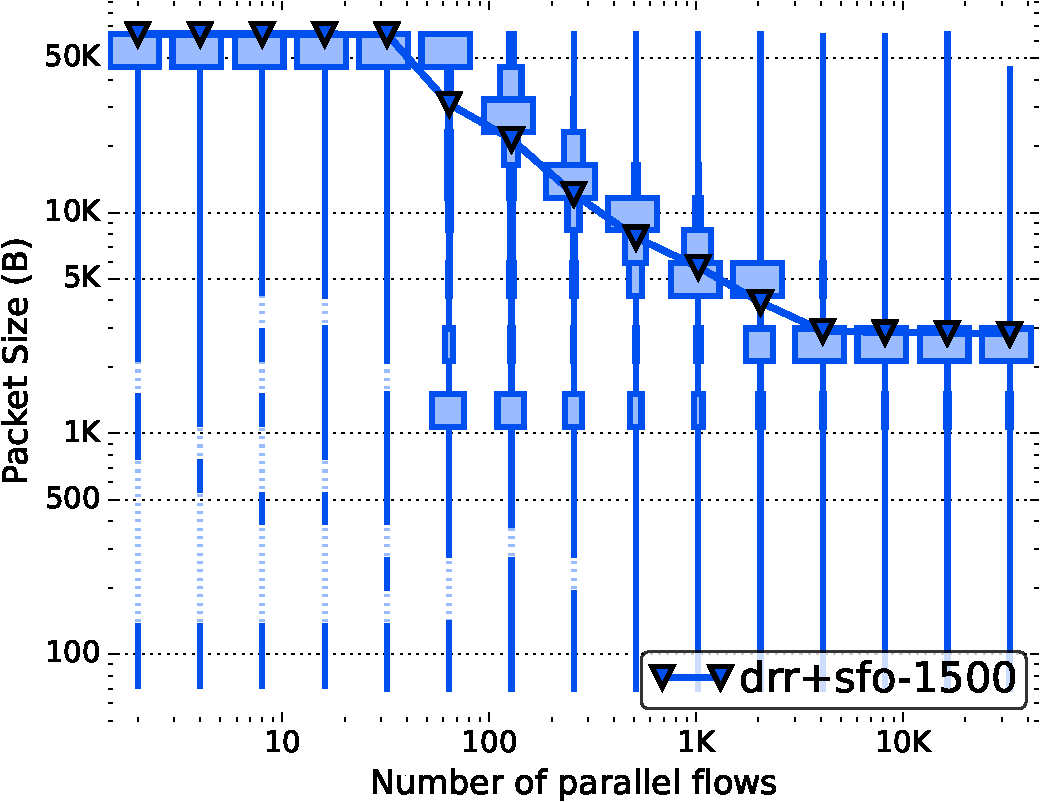
\includegraphics[width=1\linewidth]{figs/paral_cn_1t16x1024_gso_pkthist_fq_drr_1500.pdf}
        \vspace{-2mm}
        \caption{\small{\textit{TSO on TX machine}}}
	\label{fig:packets-edge}
    \end{subfigure}
    \begin{subfigure}[t]{.40\linewidth}
      \centering
      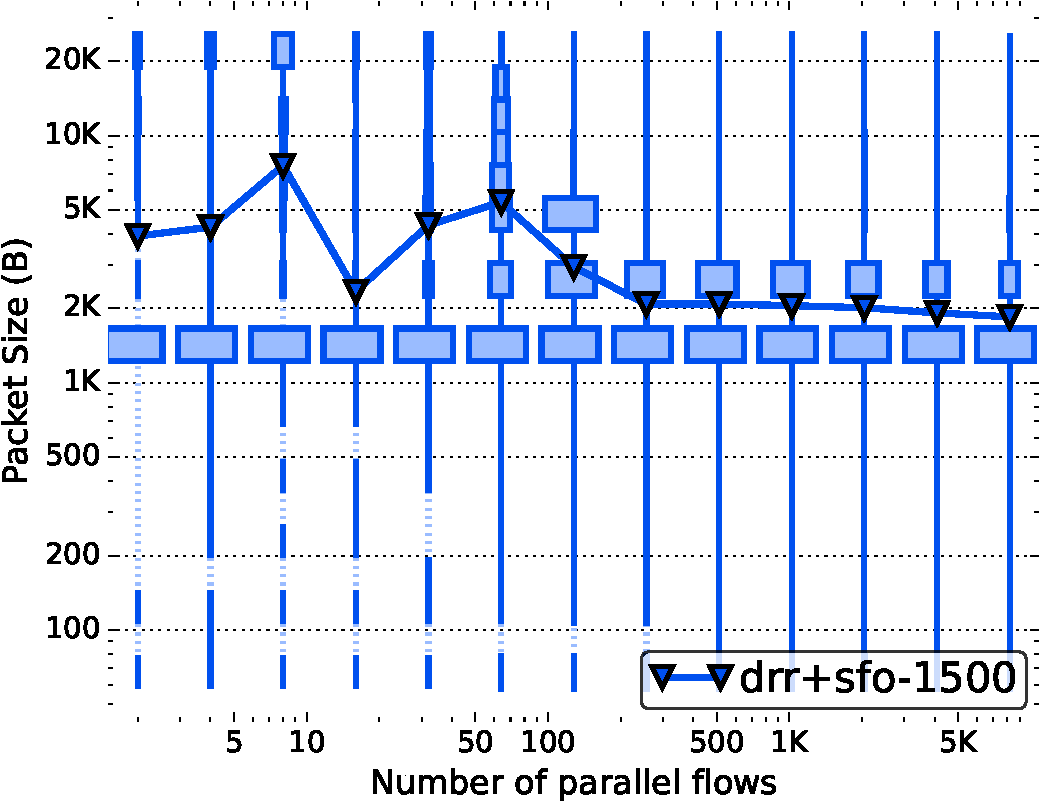
\includegraphics[width=1\linewidth]{figs/paral_cn_1t4x1024_gro_pkthist_fq_drr_1500.pdf}
      \vspace{-2mm}
      \caption{\small{\textit{LRO on RX machine}}}
      \label{fig:packets-core}
    \end{subfigure}
    \vspace{-1mm}
    \caption{\small{
        SKB length distribution under NIC offloading functions. 
    }}
    \label{fig:packets}
    \vspace{-2mm}
\end{figure}





\subsection{The Amplifying Impact of Packet Sizes}
\textbf{Packet lengths are diverse in today's networks.}
Recent studies report a wide range of
values for packet length distributions observed in the network
\cite{social,high-resolution,wild,caida,im}. Fig. \ref{fig:packets-wild}
presents the packet size distribution for the Internet traces.
According to these studies, heavier workloads such as instant
messaging (\textit{im}) tend to transmit MTU-sized packets while mixed
workloads such as \textit{mawi} send a wider range of packet sizes
with a considerable number of short packets in the mix.  The available
backbone traffic packet traces \cite{caida} further highlight that
packet length distribution constantly alternates in short periods
(e.g., between bursts of 550B, 1500B, and 60B segments).  Many modern
interactive applications use small packets to reduce latency and to
minimize the impact of packet loss, while some even adapt their packet
sizes based on performance feedback \cite{webrtc-teams, zoom-quality}.
The quantum for DRR needs to be set based on the packet size \cite {drr},
which makes it even harder for operators to tune their fixed
quantum scheduler since these variations in packet lengths are not
only workload-dependent but also volatile in the short term.
\\
\textbf{Hardware offloads and large packet buffers make it difficult to configure quanta.}
Software network stacks rely on offloading support in the
network interface (NIC) to keep up with their increasing bandwidth
\cite{overheads}. On the transmit side, \textit{Transmit Segmentation
Offload} (TSO) breaks large Socket Buffers (SKBs) into MTU-sized packets in
the NIC \cite{linux-gso-gro}. On the receiving side, \textit{Large
Receive Offload} (LRO) aggregates small segments into
larger frames \cite{linux-gso-gro}. In Linux, by default, the SKB size
can run as high as 64~kB and with proposals to greatly increase
this maximum \cite{big-tcp}. The reduction in SKB rate provided by TSO
and LRO improves software performance by reducing the overhead of
context switches, cache misses, and metadata handling. However, TSO
and LRO force any software packet scheduler to deal with a wide and unpredictable range of packet sizes.

\begin{figure}[t]
    \centering
    \begin{subfigure}[t]{.40\linewidth}
        \centering
        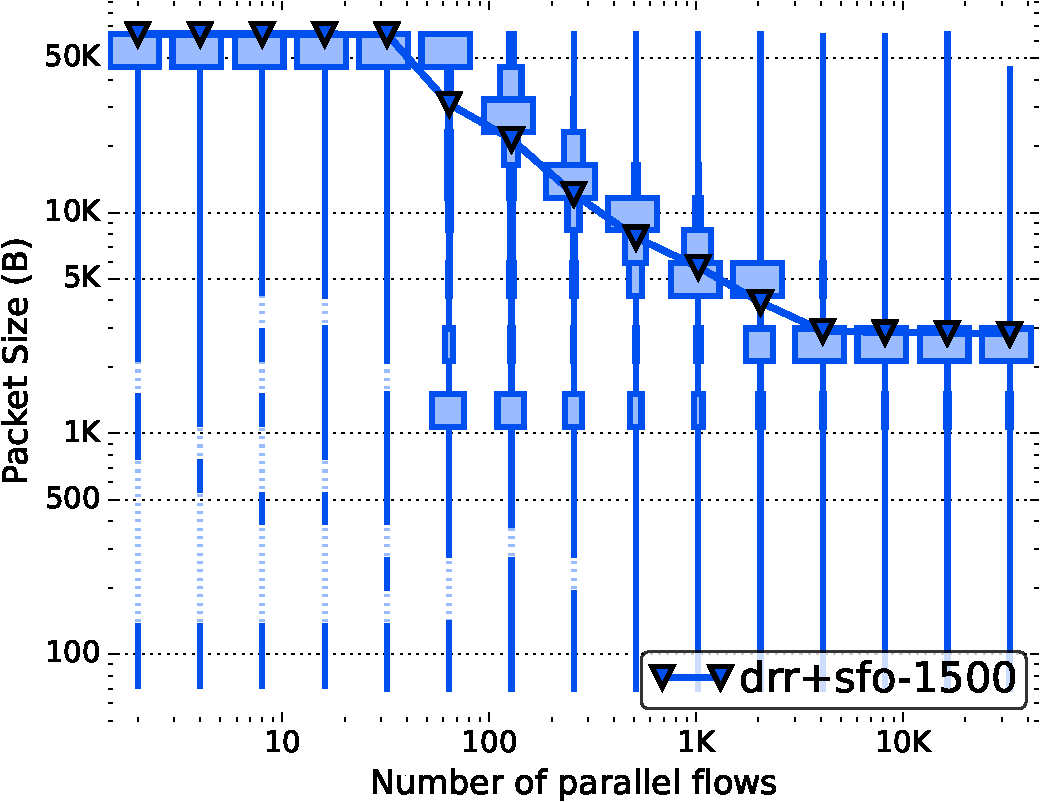
\includegraphics[width=1\linewidth]{figs/paral_cn_1t16x1024_gso_pkthist_fq_drr_1500.pdf}
        \vspace{-2mm}
        \caption{\small{\textit{TSO on TX machine}}}
	\label{fig:packets-edge}
    \end{subfigure}
    \begin{subfigure}[t]{.40\linewidth}
      \centering
      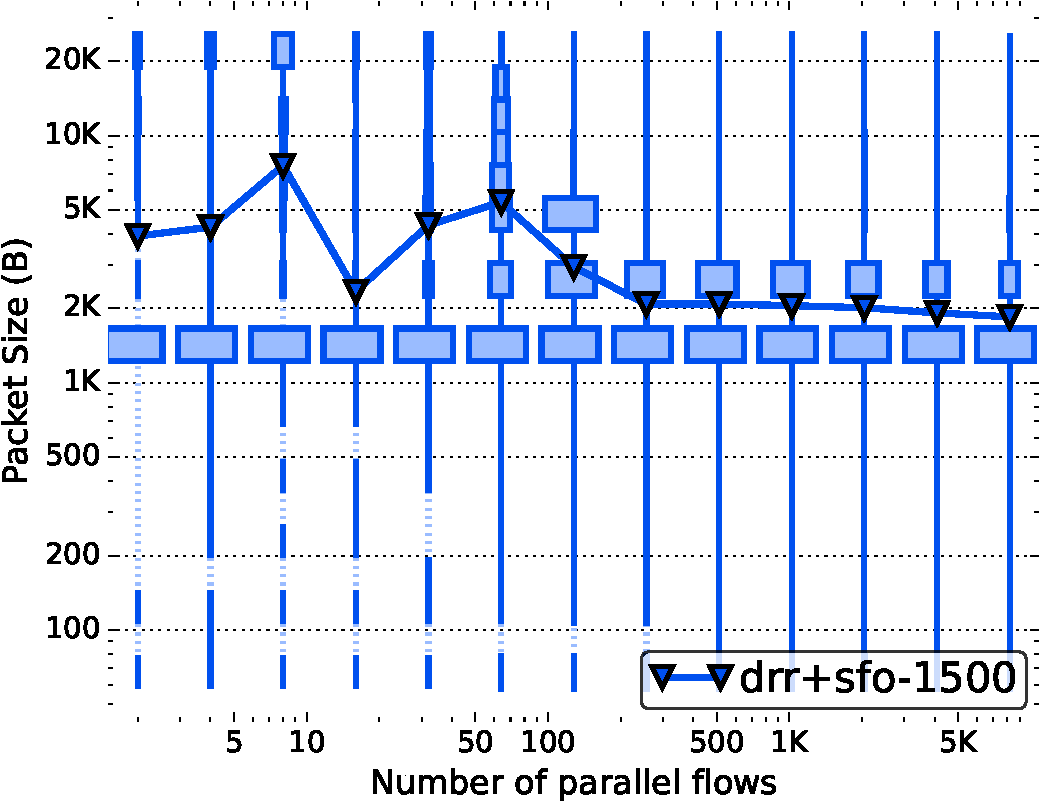
\includegraphics[width=1\linewidth]{figs/paral_cn_1t4x1024_gro_pkthist_fq_drr_1500.pdf}
      \vspace{-2mm}
      \caption{\small{\textit{LRO on RX machine}}}
      \label{fig:packets-core}
    \end{subfigure}
    \vspace{-1mm}
    \caption{\small{
        SKB length distribution under NIC offloading functions. 
    }}
    \label{fig:packets}
    \vspace{-2mm}
\end{figure}



% This is a relatively large quantum value for schedulers such as DRR as it leads to very large bursts of packets from the same flow on the wire and increases the overall latency of flows as we will observe later in this study.
% However, if the fair-queuing scheduler implemented as a qdisc class is configured with a smaller quantum setting, such large SKBs will incur missed scheduling on the system, increasing CPU utilization by doing idle work. On the other hand, a large quantum setting will have two negative outcomes. First, it will allow each individual flow to send a large burst of packets, losing the opportunity to interleave smaller packets of different flows. Second, with a large quantum the disparity in bandwidth allocation to flows results in short-term unfairness.

For packet schedulers deployed as part of virtual switches in the datacenter or cloud, the
packet size distribution will be dictated by
\textit{TSO}. Figure \ref{fig:packets-edge} presents the packet size
distribution of experiment \S\ref{sec:scrr-eval-gsogro}, in the form of
parallel histograms (wider bins indicate higher occurrence and the
straight horizontal line presents the average packet size over the
number of parallel flows) as received by the packet scheduler for
different numbers of concurrent \textit{Iperf} flows generated on that
server. With more flows, TSO tends to generate smaller packets, as
each flow has a smaller bandwidth and TSO tries to match the smaller
bandwidth delay product.

% Finally, since we use jumbo MTU frames, the distribution of packet sizes tends to center around multiples of 9K frames.

For packet schedulers that are part of home routers, SD-WAN gateways, access
points or middleboxes, the packet size distribution will be dictated
by \textit{LRO}. Fig. \ref{fig:packets-core} presents the packet sizes
generated by LRO for experiment \S\ref{sec:scrr-eval-gsogro}. LRO causes
less aggregation than TSO, but is also less predictable, likely due to the
interplay of LRO with actual packet arrivals at the NIC and NIC
interrupt coalescence. TSO and LRO make it harder to set the quantum
optimally, and a quantum greater than the largest packet size, 64~kB,
is much too large in most cases.

% Nevertheless, the shape of the distribution shifts with the number of parallel flows, suggesting that a single quantum setting for DRR might be far from optimal for the scheduler's operations.

\textbf{Mis-configuration with Jumbo Ethernet.}  Many network devices
may not be optimally configured, or are configured
conservatively. Most end hosts are configured for standard Ethernet,
in case a network device does not support Jumbo packets. If a network
devices enables support for Jumbo Ethernet \cite{jumboixp}, e.g., in
case some end-hosts need it, then DRR on this device would use a 9~kB
quantum when the MTU is effectively 1500~B.

% Some network devices even use a hardcoded 9~KB quantum
% for DRR, regardless of the Jumbo Ethernet configuration. \todo{reference}

% \begin{figure}[t]
    \centering
    % 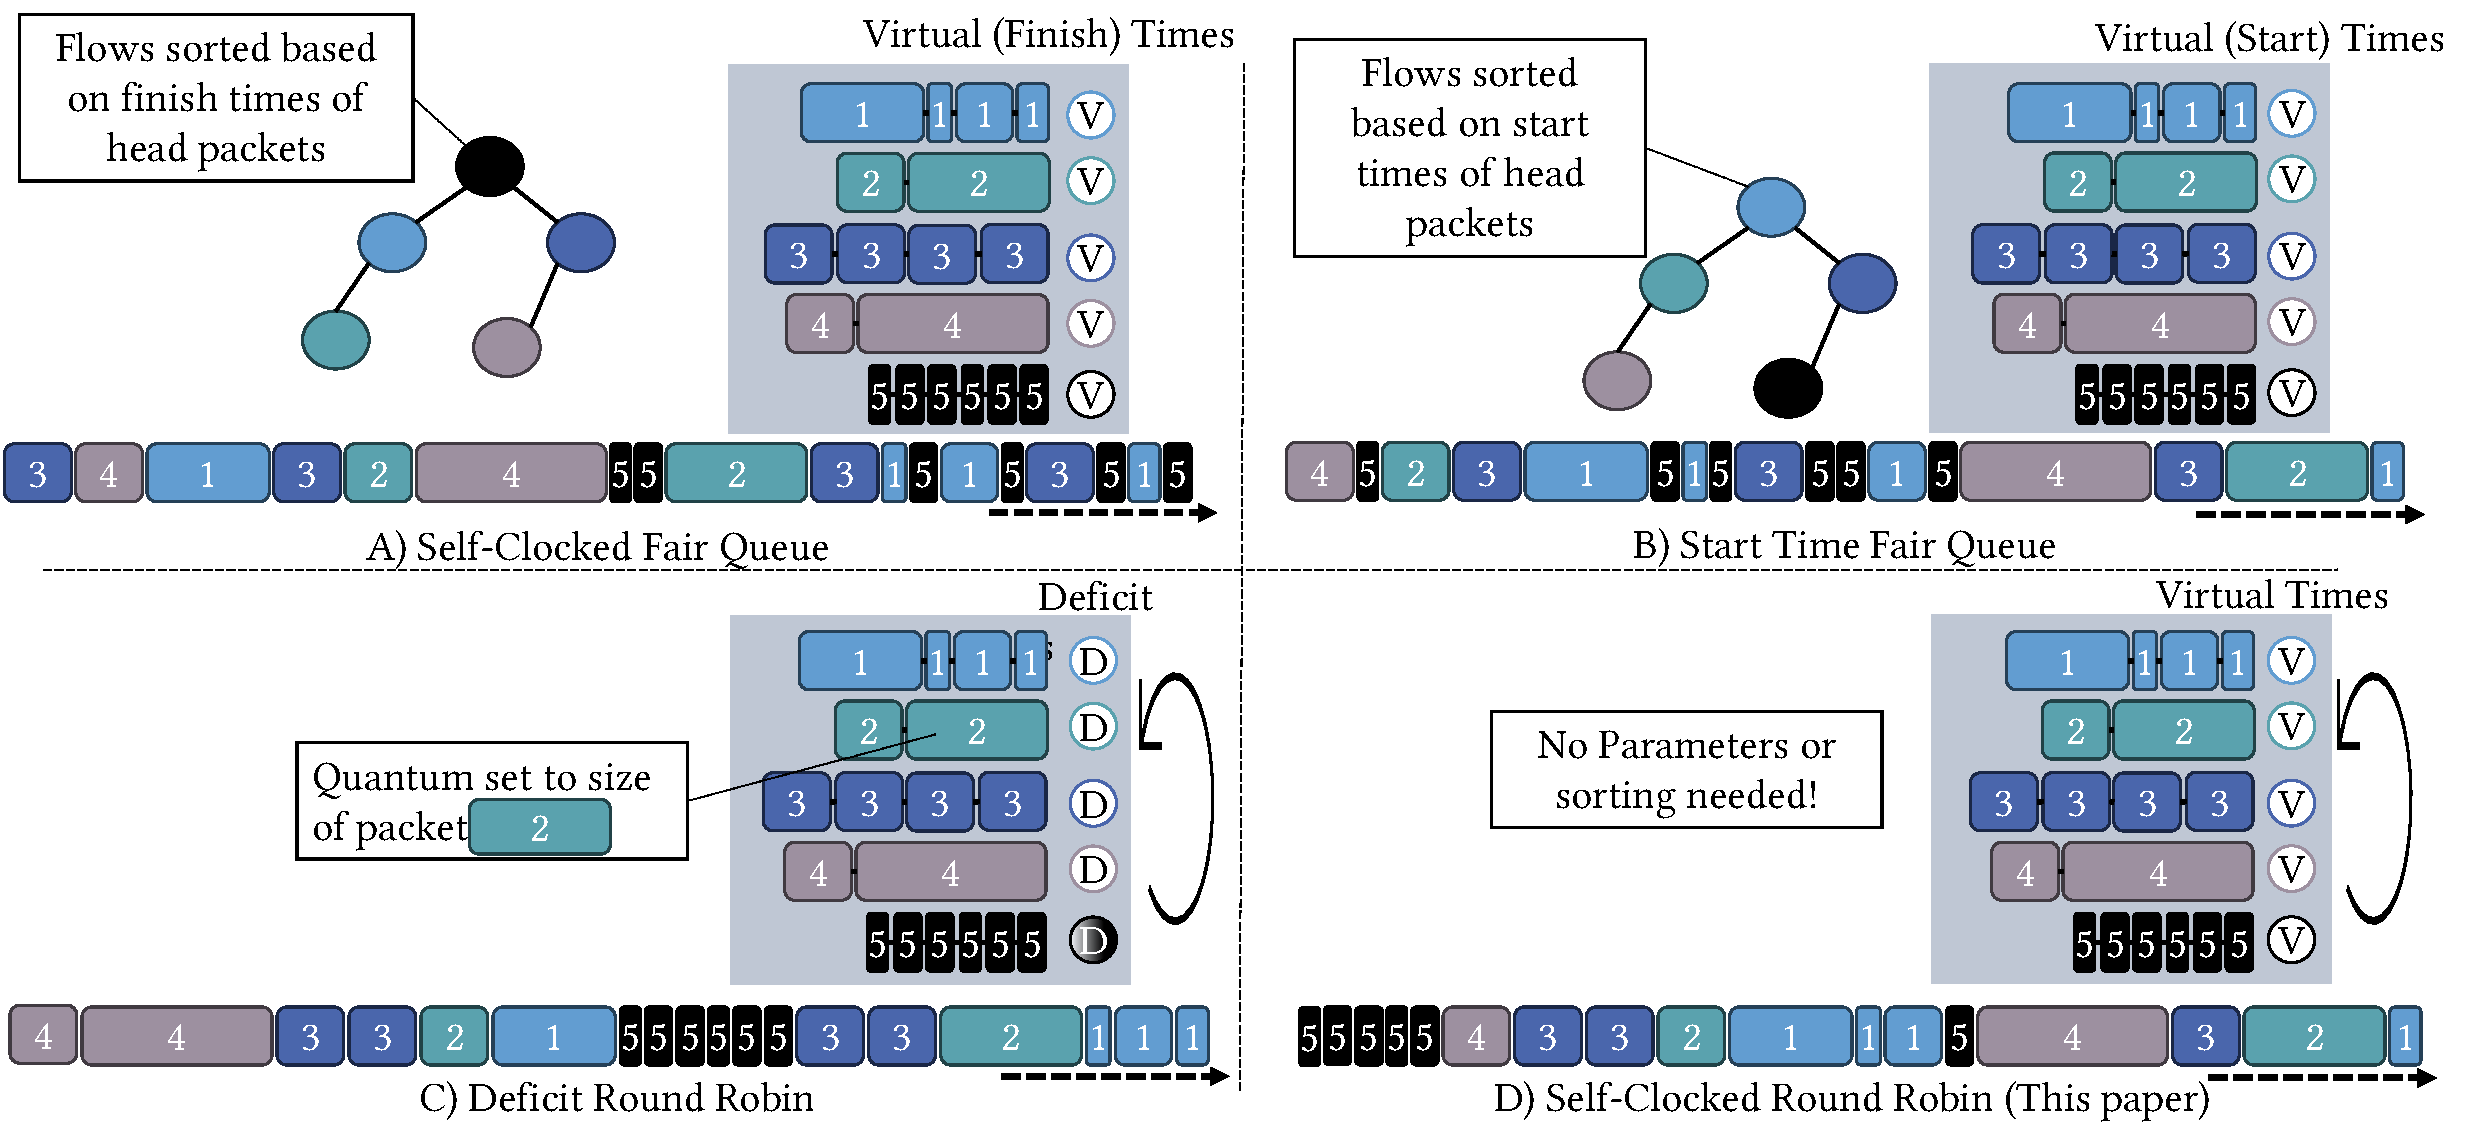
\includegraphics[width=0.99\linewidth]{figs/demo-scrr.pdf}
    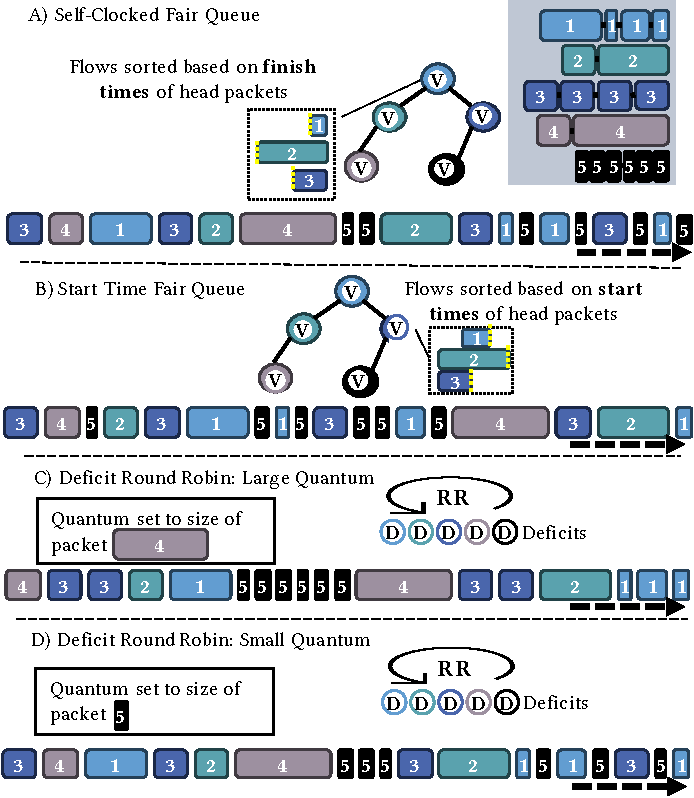
\includegraphics[width=0.85\linewidth]{figs/demo-scrr2-crop.pdf}
    \vspace{-4mm}
    \caption{\small{\textit{Output of four representative scheduling algorithms under an example scenario.}}}
	\label{fig:demo}
 \vspace{-5mm}
\end{figure}



\subsection{DRR Quantum Configuration Trade-offs}
\label{sec:drr-tradeoff}

\begin{figure}[t]
    \centering
    \begin{subfigure}[t]{.49\linewidth}
        \centering
        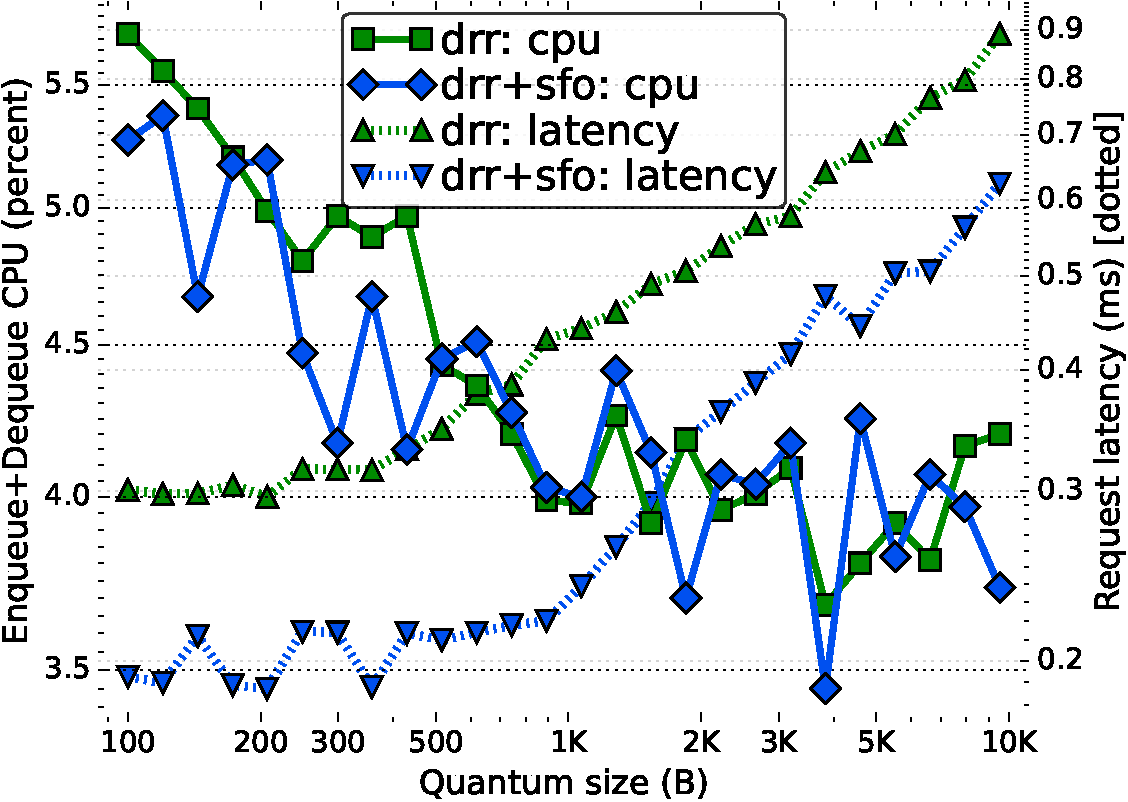
\includegraphics[width=1\linewidth]{figs/burst_cn_2t4x8_mn_2tb2x4_crs_500_kp_lat_drr_basic_fq_drr.pdf}
        \vspace{-2mm}
        \caption{\small{\textit{CPU vs scheduling latency}}}
	\label{fig:quanta-cpu-lat}
    \end{subfigure}
    \begin{subfigure}[t]{.49\linewidth}
      \centering
      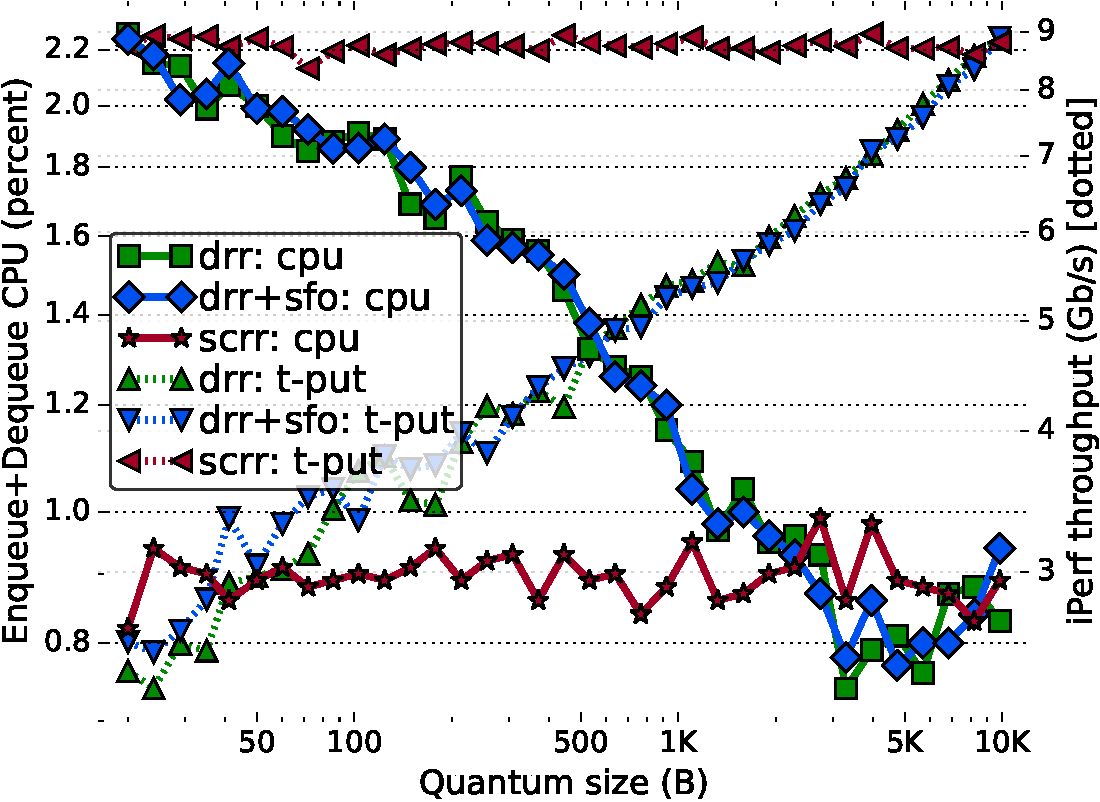
\includegraphics[width=1\linewidth]{figs/burst_cn_6u1x100_Cb_2G_kp_bw_drr_basic_fq_drr_scrr-neia.pdf}
      \vspace{-2mm}
      \caption{\small{\textit{CPU vs app. throughput}}}
      \label{fig:quanta-cpu-bw}
    \end{subfigure}
    \vspace{-1mm}
    \caption{\small{
        Trade-offs in DRR's quantum configuration.}}
    
    \label{fig:quanta-tradeoff}
    \vspace{-2mm}
\end{figure}




DRR's quantum is usually set to the maximum packet size in the network
(MTU) \cite{drr}. Such configuration impacts application performance
and resource utilization.  With a large quantum, \textit{DRR} produces large
bursts of packets that belong to a single flow and a latency-sensitive
flow has to wait longer to be allocated its share, increasing the
application latency (Figure \ref{fig:drr-burst-latency}). Conversely,
with a quantum smaller than MTU, DRR may need to spend a few
scheduling rounds accumulating enough deficit to transmit a large
packet, such missed visits ultimately result in wasted compute
resources.\footnote{Some hardware implementations of \textit{DRR} use negative
deficits, however after sending a large packet, missed visits will be
needed to recover the deficit and avoid unfairness. The only way to
eliminate missed visits is either to accept unfairness or to restrict
the quantum to be greater than MTU.}  Figure \ref{fig:quanta-cpu-lat}
presents the results of an experiment with the \textit{DRR} scheduler mixing
latency-sensitive 500B requests traffic (a two packet burst) with
heavy background traffic using 1500B packets as an attempt to mimic
the mixed and diverse nature of Internet bursts arriving at
a bottleneck (the experiment is fully described in
\S\ref{sec:scrr-eval-latency}).  Increasing the quantum to 10 kB increases
the latency of the small requests experienced at the application level
(by 140\% compared to the best-case latency for \textit{DRR+SFO}). Reducing the
quantum to 100B raises the CPU utilization of the scheduler to nearly
7\% of the system (around 75\% increase), in this case 93\% of its
scheduling visits are missed due to insufficient deficit.


CPU utilization is a good proxy for the overall resource requirements
of the packet scheduler. Some software implementations of packet
schedulers in Internet gateways result in reduced network throughput
due to their high CPU usage \cite{cake-perf1, cake-perf2}.
Figure \ref{fig:quanta-cpu-bw} shows an incast of heavy flows sharing
a bottleneck link serviced by \textit{DRR} as we increase the CPU
utilization by reducing the quantum. We use \textit{perf} to
measure the CPU consumption of the scheduler's qdisc module. At
higher quanta, the lower per-packet processing time is balanced by the
increasing packet rate, and CPU usage is constant. A small 20B
quantum makes \textit{DRR} the bottleneck and reduces aggregate
throughput to 3 Gb/s, which is a third of the capacity. The CPU usage for
\textit{DRR} is less than 2.5\%, however this puts enough pressure on
the rest of the networking stack to cause such a slowdown. During
packet processing many other parts of the Linux network stack must be
exercised that respectively consume CPU. With more pressure on the
qdisc, the network stack processing also experiences more CPU
contention and cache pressure.

%Round-robin scheduling is easy to implement and is compatible with multi-core and multi-pipeline data paths although there is no correct answer to its configuration trade-offs. \textit{An ideal packet scheduler for fair queueing should adapt to workload changes both at flow and packet-level without the need for explicit user input.  In addition, a widespread deployment requires scalability, resource-efficiency, and tight bounds on both performance and fairness.} 
% The next section introduces such a scheduler.

% The above observations hint that all the varieties of widely deployed fixed-quantum round-robin packet schedulers face performance trade-offs when confronting everyday workloads. These trade-offs challenge the efficiency and practicality of this scheduling paradigm of old in low-latency and resource-constrained environments. On the other hand, the classical fair queueing paradigms rely on parameter-less self-clocking semantics with strong performance and fairness bounds.\textit{ If only we could revive and reuse these fair queueing systems in large-scale deployments, we would realize a packet scheduler that is resource-efficient, low-latency, scalable to a high number of incoming flows, and has strong fairness bounds.} The next section introduces such a scheduler.

%  \textbf{Summary.} Looking back at existing proposals on fair packet scheduling, a trade-off can be perceived between fairness properties, scalability to large number of flows, and latency. With the dynamic nature of today's data center workloads that feature skewed packet length distributions, widely deployed packet scheduling paradigms can suffer from poor configuration which consequently results in degraded performance e.g., increased latency and reduced throughput as well as higher resource consumption. In the following section, we study these effects in more detail.

% \subsection{Multi-Queue Fair Queueing}
% As higher 100 Gbps networks become commodity and 400 Gbps and 800 Gbps devices are introduced, the gap between software and hardware packet processing starts to widen. 
% While a single CPU core has been more than enough to perform packet processing at 10 Gbps line rates, software pipelines struggle to perform either ingress or egress processing for higher link rates on a single core. The existing Linux kernels implement a hierarchical multi-queue traffic control layer that allows individual packet schedulers to work concurrently on multiple cores and delegate the last level of scheduling decisions to a fixed-function DRR scheduler at the NIC \cite{loom,titan,valinor}.
% Alternatively, MQFQ \cite{mqfq} introduces a fair queueing scheme, mainly optimized or storage schedulers, that can synchronize concurrent fair queueing schedulers on multiple cores in order to provide a more fair scheduling paradigm.

% \textbf{Scalable packet scheduling.}
% As the performance gap between software and hardware widens, software packet processing struggles more to drive line-rate performance due to the limited processing power that is offered by a single CPU core. Subsequently, multi-queue packet scheduling has become a standard with high-performance networking hardware which allows multiple instances of packet scheduler to run in parallel across cores \cite{titan,loom}.
% Alternative approaches like MQFQ \cite{mqfq} aim to realize a centralized scheduler that is shared between CPU cores and can accurately maintain fairness, even for workloads that span multiple CPUs. However, the scalability of single-core processing can still prevent them from scaling to multi-hundred-gigabit networks.


\section{Self Clocked Round Robin}
\label{sec:scrr-design}


An ideal packet scheduler should adapt to workload dynamics, such as
varying packet sizes and burstiness, both at the flow and packet
level, without the need for explicit user input. Conversely, DRR
requires quantum configuration based on packet lengths and flow
types.  In addition, a widespread deployment requires scalability,
resource efficiency, and tight bounds on both performance and
fairness, which cannot be satisfied altogether by Fair Queuing
schedulers. In this section, we introduce \textit{Self-Clocked
Round-Robin Scheduling (SCRR)} to address those needs. We design SCRR
with the following goals in mind:

\begin{compactitem}
    \item Per-flow or per-class QoS scheduling.
    \item Fair bandwidth allocation.
    \item Low scheduling latency for bursty flows.
    \item Low resource consumption at high loads.
    \item Scalability to large number of sub-queues.
    \item Compatibility to any transport, including TCP.
    \item Parameter-less and agnostic to flow information.
    \item Plug and play replacement for DRR and Fair Queuing.
\end{compactitem}


To envision SCRR, we find that virtual clocking proves to be a great asset in realizing
dynamic scheduling paradigms that adapt to workload changes. Unlike
conventional deficit round-robin that sends a predetermined burst on
each sub-queue visit, SCRR aims to track virtual times for sub-queues
and transmit as much as a flow sub-queue's virtual time allows in
order to achieve fair scheduling without relying on any flow
information. In order to eliminate the expensive ordered list
maintenance as in classical fair scheduling \cite{scfq,stfq}, SCRR
visits each flow sub-queue in a round-robin fashion. SCRR can be used
in both low-load and high-load environments as a parameter-less
improvement over DRR. (\S\ref{sec:scrr})

SCRR is flexible and is augmented by various customizations and
enhancements. SCRR can optionally use weight for the sub-queues
(\S\ref{sec:scrr}) \cite{wfq}. It can use the \textit{virtual finish time}, like
SCFQ \cite{scfq}, or \textit{virtual start time}, like STFQ
\cite{stfq}. \textit{No Packet Metadata} (\S\ref{sec:npm}) eliminates
the need to tag packets with their virtual time while enqueued,
reducing resource requirements. The combination of \textit{Sparse Flow
Optimization} (\S\ref{sub:sfo}), \textit{Initial Advance}
(\S\ref{sub:initial-advance}), and \textit{No Empty}
(\S\ref{sub:no-empty}) use the properties of virtual time to decrease
the latency of bursty flows beyond the state of the art, without
violating the fairness and burstiness guarantees of SCRR. With these
enhancements, when both heavy and short flows are present at the
scheduler, bursty flows will not have to wait for multiple scheduling
rounds to make progress and enjoy lower scheduling latency.

%SCRR can therefore offer fairness, responsiveness, resistance to head-of-the-line (HoL) blocking and low scheduling latency for bursty latency-sensitive flows (\S\ref{sec:enhancements}).

%Additionally, SCRR offers low latency for bursty, latency-sensitive flows through careful virtual time adjustment when flows become active after a period of idleness, without violating their fairness bounds. This mechanism ensures that when both heavy and short flows are present in the scheduler, short flows will not have to wait for multiple scheduling rounds to make progress.

%Next, we explore the self-clocking traits that realize SCRR without the need to maintain per-packet metadata (\S\ref{sec:npm}). The final contribution in designing SCRR is identifying the design trade-offs for different types of flows with respect to their size and performance requirements. While the original design of SCRR realizes fair bandwidth allocation for backlogged flows, it also sets the stage for additional enhancements aimed at ensuring responsiveness, head-of-the-line (HoL) blocking prevention, and ultimately low scheduling latency for bursty latency-sensitive flows (\S\ref{sec:enhancements}). 
% SCRR is an attractive scheduler for hardware targets as it can be implemented without the need for per-packet metadata. We explore this variant in \S\ref{sec:npm}. 

\begin{table}[]
\centering
% \caption{\small{Mathematical notations used for theoretical attribution of SCHYS.}}
\caption{\small{Description of mathematical notations for SCRR.}}
\vspace{-3mm}
\label{tab:notations}
\resizebox{0.6\linewidth}{!}{
\begin{tabular}{l|l}
\rowcolor[HTML]{DAE8FC} 
{\color[HTML]{000000} \small{Notation}} & {\color[HTML]{000000} \small{Description}} \\ \hline
  \small{$p_f^j$}  &   \small{Packet $j$ of flow $f$}       \\ \hline
    \small{$l(p_f^j)$}  &  \small{Length of packet $p_f^j$}  \\ \hline
  \small{$c(k)$}  &   \small{Global virtual clock at scheduling round $k$}       \\ \hline
   \small{$v(p_f^j)$}   &   \small{Virtual time of packet $(p_f^j)$}       \\ \hline
     \small{$r_f$}  &  \small{Rate (weight) of flow $f$}   \\ \hline
     \small{$N$} & \small{Number of packets in the scheduler} \\ \hline
     \small{$Q$} & \small{Vector of active sub-queues in the scheduler} \\ \hline
     \small{$n$} & \small{Number of active sub-queues in the scheduler} \\ \hline
     \small{$M$} & \small{Maximum length among all packets} 
\end{tabular}
}
\vspace{-2mm}
\end{table}



\subsection{Virtual Clocking Semantics}
\label{sec:scrr}

We start by laying out the formal foundations of the SCRR
scheduler. All mathematical notations used are summarized in Table
\ref{tab:notations}. The SCRR scheduler maintains a \textit{global
virtual clock}, which is updated to the maximum virtual time of dequeued
packets at the end of each round. Each sub-queue features a head
virtual time which is determined by the virtual time of the packet at
the head of the queue. Depending on the head virtual time, sub-queues can be either \textit{lagging} or \textit{leading} compared to the global
virtual clock. During each sub-queue visit, the scheduler allows
a lagging sub-queue to catch up with the global virtual scheduling
time, while a leading sub-queue advances the global virtual
clock. During a period that is longer than a scheduling round,
sub-queues may change their state from \textit{lagging} to
\textit{leading} and vice versa.


\begin{definition}
    A \textit{scheduling round} is the period of time when all active sub-queues have been visited once, and only once. A sub-queue is active when it contains outstanding packets.
\end{definition}

\begin{definition}
    A sub-queue is \textit{lagging} (catching up) as long as its head virtual time is smaller than the global virtual clock.
\end{definition}

\begin{definition}
    A sub-queue is \textit{leading} as long as its head virtual time is larger or equal to the global virtual.
\end{definition}

During each round, the scheduler visits sub-queues in round-robin and forwards all packets that have a virtual time that is older than the global virtual clock. If a sub-queue does not feature a lagging packet, the head packet is transmitted, and the scheduler moves to the next sub-queue. This ensures that no processing cycle is wasted when visiting each sub-queue, while still ensuring that fairness can be achieved via virtual clocking. 
SCRR effectively implements round-robin scheduling with byte-level fairness granularity and an adaptive quantum equal to the largest serviced packet in a round.
\\
\\
\subsection{Enqueue Process}
Since SCRR is a multi-queue scheduler, the arrived packets undergo a classifier to determine their target sub-queues. In implementations that target per-flow fairness, each flow is stochastically assigned to a separate sub-queue using a flow classifier (e.g., \textit{fq} in Linux). 
If the sub-queue is backlogged, the virtual time of the tail packet plus its size is used as the virtual time for the new packet. However, if the sub-queue had been idle, the current global clock is used as the packet virtual time. This is to ensure that an idle sub-queue does not receive a large (and consequently, unfair) scheduling share due to inactivity for a long period. 


Formally, at scheduling round $k$, the virtual time of packet $p_{f}^{j}$, i.e., the $j$'th packet of sub-queue $f$, is defined as:
\begin{equation}
\label{equa:virtual-enqueue}
    S(p_{i}^{j}) = max\{F(p_{i}^{j-1}), c(k)\}
\end{equation}
where $F(p_{i}^{j})$ is the virtual finish time of the previous packet and $c(k)$ denotes the current virtual time of the scheduler.
The virtual finish time for packet $p_{i}^{j}$ is defined as:
\begin{equation}
\label{equa:virtual-previous}
    F(p_{i}^{j}) = S(p_{i}^{j}) + \frac{l(p_f^j)}{r_f}
\end{equation}
where $l(p_f^j)$ denotes the length of the packet and $r_f$ is the weight of the sub-queue $f$.
Algorithm \ref{alg:scrr-basic-enq} in Appendix \ref{app:algs} presents the enqueue procedure.
\\
\\
\subsection{Dequeue Process}
\label{sec:dequeue}
The majority of virtual timekeeping processes take place during the packet dequeue. 
SCRR starts with the first non-empty sub-queue and schedules one packet. The scheduler then loops through that sub-queue and transmits packets as long as the virtual time of the head packet is older than the global virtual clock. This approach accomplishes two key objectives. First, it guarantees the transmission of at least one packet from each sub-queue, preventing missed schedule opportunities that lead to wasted compute cycles. Second, it helps the lagging sub-queues to catch up with the leading sub-queues by sending multiple packets. Upon moving to the next sub-queue, the scheduler records the start time of the last dequeued packet and cycles through the remaining active sub-queues. When a scheduling round is finished, SCRR updates the global virtual clock to the maximum packet virtual time that was transmitted during that round. Therefore, an update of the global clock only occurs once during each round to ensure the correct operation of the scheduler. The dequeue procedure is outlined in Algorithm \ref{alg:scrr-basic-deq} in Appendix \ref{app:algs}.

The self-clocking semantics in SCRR uses Start-Time Fair Queuing (STFQ)
\cite{stfq} as its basis. Alternatively, as a design choice, it is possible to
schedule packets using their virtual finish times as in \cite{scfq}.
In \S\ref{sec:scrr-analysis}, we perform all the correctness proofs for the
\textit{start time} version, and in Appendix \ref{sub:clock-finish}, we
do the same for the \textit{finish-time} version. The two self-clocking paradigms offer identical fairness and burstiness bounds for SCRR and differ slightly in the state-keeping required for the scheduler's implementation. 
It is also worth noting that all virtual time calculations in SCRR support sub-queue weights to implement QoS, i.e., the packet's length is divided by the weight of its corresponding sub-queue. 

% For brevity, we opted to omit weights from our analysis.

% The Appendix also
% showcase three improvement to the basic SCRR. \textit{No Packet
% Metadata} (\S\ref{sub:no-packet-metadata}) move computation of virtual
% time to the dequeue process, eliminating the need for per-packet
% metadata and associated memory operations. \textit{No Empty}
% (\S\ref{sub:no-empty}) remove sub-queues from the schedule as soon as
% they are empty, eliminating schedules where a queue is empty and the
% associated CPU overhead and cache pollution. \textit{Full Advance}
% (\S\ref{sub:full-advance}) set the virtual time of newly active
% sub-queues to the global clock of the previous round, instead of the
% current round, to allow latency sensitive flows to send multiple
% packets in their first scheduling round.

\subsection{Eliminating Per-packet Metadata}
\label{sec:npm}

Both SCFQ \cite{scfq} and STFQ \cite{stfq} need to store the virtual time of the packet while
the packet is enqueued. Since this is usually done in the packet
metadata, it has the downsides of added complexity and increased memory operations. \textbf{No Packet Metadata} (NPM) is an enhancement to 
the SCRR algorithm that computes packet metadata after dequeuing the
packet, and therefore eliminates the need to store the virtual
time of the packet as metadata.

When dequeuing a packet, the first issue is to know if the sub-queue
was idle or backlogged when the packet was enqueued
(\S\ref{sec:scrr}). With \textbf{NPM}, the scheduler saves the global
virtual clock of the previous round. If the virtual time of the last
dequeued packet in the sub-queue is greater than previous virtual
clock, then that sub-queue was scheduled in the previous or current
round, and was backlogged. When a sub-queue is backlogged, the start
time of any queued packet can be derived from the finish time of its
predecessor in the sub-queue. Consequently, the sub-queue must store
the finish time of the last dequeued packet, instead of the finish
time of the last enqueued packet. When a sub-queue was idle, NPM
always sets to virtual time of the packet to the current global
clock. When the sub-queue was idle, the packet virtual time is
supposed to be the value of the global virtual clock at the time the packet
was enqueued (Equation \ref{equa:virtual-enqueue}). The insight is
that in SCRR, precise virtual timing does not really matter as long as
the packet is included in the proper scheduling round and its virtual
time does not change the computation of the next global
clock. Further, in many cases the sub-queue was added to the schedule
in the current round, so the packet virtual time would have been the
current global clock anyway.

\textbf{NPM} computes the virtual time of dequeued packets
based on the scheduler's previous global time and the previous
packet's finish time in the same sub-queue. This simple heuristic
makes SCRR as memory efficient as DRR while making the enqueue process
a breeze by removing four memory operations during insertion. The
theoretical proofs obtained for SCRR also apply to SCRR with NPM,
using either the finish time of packets or their start times.

\subsection{Flow Latency Enhancements for SCRR}
\label{sec:enhancements}
\label{sec:latency}

Packets of \textit{backlogged flows} need to wait for all prior
packets of the sub-queue to be dequeued, so their queuing delay is the
sub-queue's length times the duration of each scheduling round. The
latency of such packets is dominated by the queuing delay, therefore
their exact position in the scheduling round has little impact on
their latency. Further, backlogged flows are usually associated with
throughput-intensive applications whose performance is dictated by the fairness of the scheduler. For
backlogged flows, round robin schedulers, such as DRR and SCRR, are in
practice as good as Fair Queuing schedulers, such as SCFQ and STFQ.

Non-backlogged flows, also called \textit{sparse flows}, don't
accumulate packets in the sub-queue, therefore, their packets are immediately
eligible to be dequeued. The position of those packets in the
scheduling round makes a big difference to their latency. Further,
interactive and latency-sensitive applications are major origins of sparse flows, or flows that alternate between sparse and lightly backlogged. Our
aim is to make the latency of SCRR for sparse flows as good as the Fair Queuing schedulers.

Our enhancements for SCRR reduce the latency of \textit{sparse flows},
and as a result make the latency of backlogged flows slightly worse
than DRR. As pointed above, backlogged flows are almost never
sensitive to such minor differences in latency. This design choice aims
to improve the latency of flows that care the most about it. This
enables to balance the scheduling performance for various 
types of flows without explicit flow information.\footnote{The
Completely Fair Scheduler is a relevant case study. While the original
process scheduler design heavily depended upon the use of nice values
for latency-sensitive processes, the scheduler was gradually improved
to automatically favor interactive applications \cite{battle}.} The
above enhancements involve various trade-offs between resource usage,
latency, and fairness. Hence, it is at the discretion of the network operators to decide which combination of SCRR features to use. We empirically
evaluate the direct impact of each of these enhancements on
application performance in \S\ref{sec:scrr-component}.

\subsubsection{Sparse Flow Optimization}
\label{sub:sfo}

\textbf{Sparse Flow Optimization} (SFO) is a technique developed for
DRR that reduces the latency of bursty flows by prioritizing sparse
flows \cite{sfo}. \textbf{SFO} was trivially added to SCRR. In
\textbf{SFO}, sub-queues that were previously inactive (i.e. sparse)
are no longer added at the back of the schedule, but instead in the
\textit{new list} of sub-queues that always take precedence over the
\textit{old list} of sub-queues (that were already part of the
schedule, i.e. backlogged). To prevent sparse sub-queues from starving
backlogged sub-queues, newly empty sub-queues are kept in the schedule
and are only potentially removed from it during the next scheduling round
\cite{formal}.

% \begin{figure}[t]
%     \centering
%     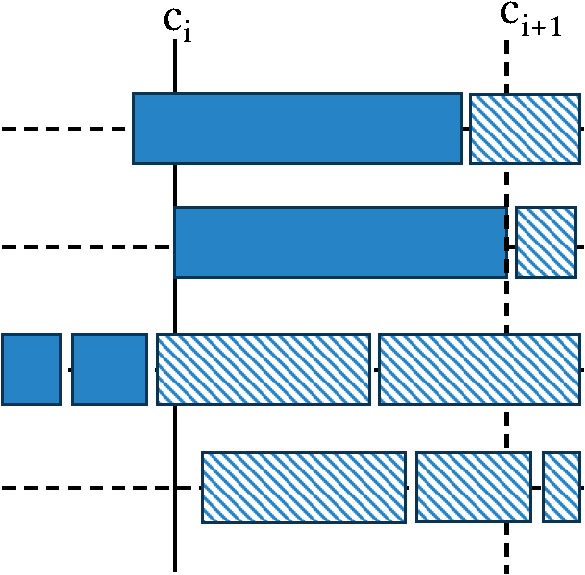
\includegraphics[width=0.6\linewidth]{figs/f1-crop.pdf}
%     \caption{\small{\textbf{Advancing global clock in SCRR.}}}
% 	\label{fig:global-clock}
% \end{figure}

% \begin{figure}[t]
%     \centering
%     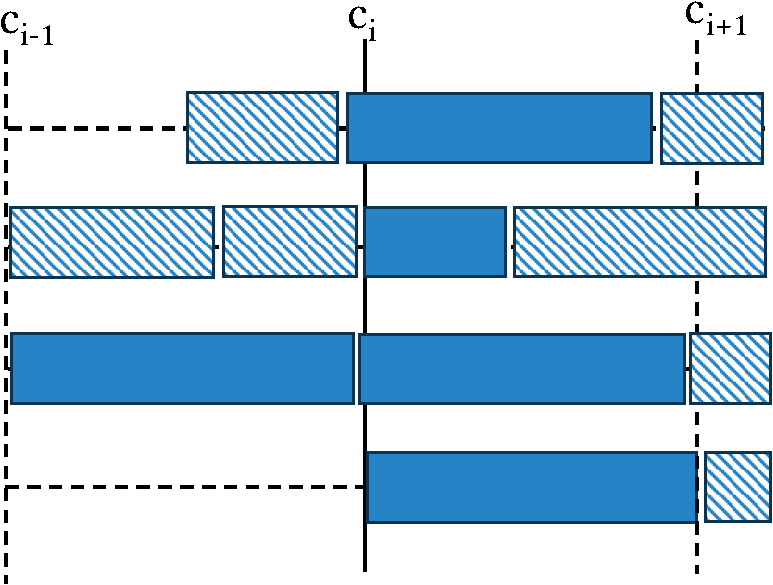
\includegraphics[width=0.6\linewidth]{figs/f2-crop.pdf}
%     \caption{\small{\textbf{Advancing the sub-queue clock in SCRR.}}}
% 	\label{fig:local-clock}
% \end{figure}

\begin{figure}[t]
    \centering
    \vspace{3mm}
    \begin{subfigure}[t]{.46\linewidth}
        \centering
        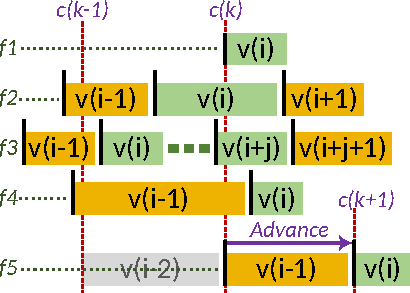
\includegraphics[width=1\linewidth]{figs/scrr-packet-advance-start.pdf}
        \caption{\small{\textit{Advancing global clock}}}
    	\label{fig:global-clock-start}
    \end{subfigure}
    \rulesep
    \begin{minipage}{.50\linewidth}
        \vspace{-20mm}
        \centering
	\begin{subfigure}[t]{1.0\linewidth}
            \centering
            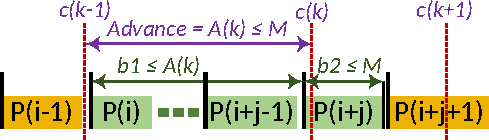
\includegraphics[width=1\linewidth]{figs/scrr-packet-burst-start.pdf}
            \vspace{-6mm}
            \caption{\small{\textit{Maximum burstiness}}}
	    \label{fig:burstiness-start}
	\end{subfigure}\\
        \vspace{1mm}
	\begin{subfigure}[t]{0.9\linewidth}
            \centering
            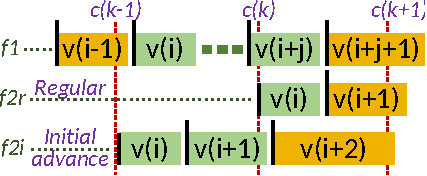
\includegraphics[width=1\linewidth]{figs/scrr-initial-advance-start.pdf}
            \vspace{-6mm}
            \caption{\small{\textit{Initial Advance}}}
	    \label{fig:initial-advance-start}
	\end{subfigure}
    \end{minipage}\\
    \vspace{-4mm}
    \caption{\small{SCRR clock management with start-time semantics.}}
    \label{fig:scrr-start}
    \vspace*{-0.4cm}

    % \hspace{10pt}
\end{figure}

% \begin{figure}[t]
%     \centering
%     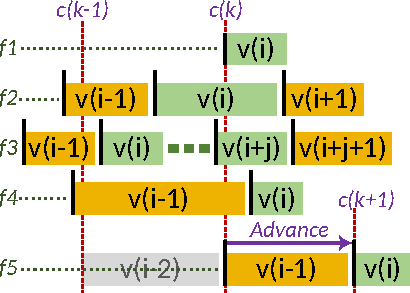
\includegraphics[width=0.6\linewidth]{figs/scrr-packet-advance-start.pdf}
%     \caption{\small{\textbf{Advancing global clock in SCRR with start-time.}}}
% 	\label{fig:global-clock-start}
% \end{figure}

% \begin{figure}[t]
%     \centering
%     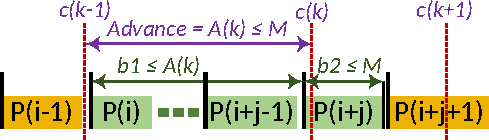
\includegraphics[width=0.6\linewidth]{figs/scrr-packet-burst-start.pdf}
%     \caption{\small{\textbf{Burstiness of SCRR with start-time.}}}
% 	\label{fig:burstiness-start}
% \end{figure}



\subsubsection{Initial Advance for new sub-queues}
\label{sub:initial-advance}

The trivial version of SFO in \textit{SCRR} does not benefit the bursty flows as
well as SFO for \textit{DRR}. With \textit{DRR}, if multiple packets have accumulated
prior to a sub-queue being scheduled via SFO, those packets can be sent
in the current scheduling round, up to a quantum. With basic SCRR, when
a sub-queue has been idle, the virtual time of the first packet is set
to the current virtual clock (same as \textit{SCFQ}/\textit{STFQ}). When the sub-queue is
scheduled with SFO, the first packet can be sent, but any subsequent
packet has a virtual time in the future and needs to wait for the next
scheduling round.

\textbf{Initial advance} fixes this issue by allowing SFO to send
multiple packets in the first schedule of a previously inactive
sub-queue. It simply sets the virtual time of the first
packet based on the previous virtual time instead of the current
virtual time (Figure \ref{fig:initial-advance-start}). The virtual time
of subsequent packets is based on the virtual time of the first packet, packet size, and the sub-queue weight, therefore setting a virtual time closer to the
previous virtual clock enables potentially more subsequent packets to
have a virtual time lower than the current virtual time, and
consequently to send more packets in the current schedule.

\textbf{Initial advance} will not violate the fairness and burstiness
properties of the scheduler. The current scheduling round processes
packets from sub-queues with virtual times later than the previous
virtual clock $c(k-1)$ (Figure \ref{fig:global-clock-start}). Therefore,
setting the virtual time of the first packet to any value later than
the previous virtual clock is still compatible with SCRR. To further prevent
unfairness and avoid starvation, SCRR makes sure that the virtual time
of a sub-queue used to tag packets can only go forward, not backward.
\textbf{Initial advance} can be further tuned. To reduce the average flow burstiness,  we set the virtual
time of the head packet to the previous virtual clock plus the packet's size times the sub-queue weight: 
if all packets in the sub-queue are the same size, the burst of
packets from the sub-queue scheduled by SFO is equal to the advance,
instead of the advance plus an additional packet 
(Figure \ref{fig:burstiness-start}).

\vspace{-2mm}
\subsubsection{Getting rid of empty visits with No Empty}
\label{sub:no-empty}



SFO in DRR keeps newly empty flows in the schedule for at least one
round to prevent unfairness and starvation \cite{formal}. This means
that the next time that sub-queue is scheduled, if it is still empty,
the scheduler needs to remove it from the schedule and pick another
sub-queue. This is problematic in software as such empty visits create
extraneous cache misses. This is also problematic in hardware with
fixed-delay processing pipelines, it makes the amount of work to
schedule one packet unpredictable, as many successive empty sub-queues
may need to be processed.

\textbf{No Empty} improves SFO and eliminates these empty visits by
leveraging the virtual clocking semantics. With \textbf{No Empty},
idle sub-queues are never kept in the schedule. To prevent starvation,
when a previously inactive sub-queue needs to be inserted into the
schedule, its virtual time is checked against the current clock. If
a sub-queue has transmitted more than its fair share of packets in the
current schedule, its virtual time will have advanced beyond the
global virtual clock. If a sub-queue has a virtual time greater than
the global virtual clock, it is denied the use of SFO, and is instead
added to the back of the \textit{old list} of sub-queues, similar to
the original DRR. Otherwise, it can use SFO and is added at the back
of the \textit{new list} of sub-queues.

\textbf{No Empty} is especially attractive to hardware implementations
as it makes the processing of SCRR with SFO completely deterministic,
without loops and recursions. It also combines with \textbf{Initial
advance} to benefit bursty flows. In many cases, the packets of the
burst do not arrive at the same time. With the original SFO, only
the packets already accumulated prior to SFO scheduling are sent in
the current schedule, if a packet arrives later, the sub-queue is at
the back of the schedule and the packet has to wait a full scheduling
round. With \textbf{No Empty}, when this later packet arrives, the
sub-queue is inactive, and can be inserted in the current scheduling
round another time, as long as the virtual time of the packet is older
than the current virtual clock.


\section{Theoretical Analysis}
\label{sec:scrr-analysis}

In this section, we explore the theoretical properties of the scheduler and provide upper bounds for the throughput, fairness, and burstiness.

\subsection{Analysis of Backlogged SCRR}
\label{sec:proofs}
% This section aims to investigate the theoretical bound for the SCRR scheduler. 
Initially, we show that the movement of the global clock under SCRR is tightly bounded during each scheduling round. Next, using this insight, we establish the fairness index of the backlogged scheduler and argue that SCRR enjoys the same fairness index as DRR in the long run. Finally, we argue that the per-flow burst sizes are strictly bounded by two maximum-sized packets, similar to DRR.


\begin{definition}[\textbf{Single Clock Update per Round}]
\label{def:onlyonce}
For the smallest time interval $[t_1, t_2]$ that includes a full round-robin scheduling round, i.e., a period when all active flows are visited at least once,
SCRR global clock is updated only once according to the scheduled packet with the highest virtual time value.
\end{definition}

\begin{definition}[\textbf{SCRR Global Clock Updates}]
\label{def:correct}
All global clock updates in SCRR occur at the end of a scheduling round, the global clock only advances forward, and the clock update marks the start of a new scheduling round.
\end{definition}


\begin{theorem}[\textbf{The Global Clock Advance Upper Bound}]
\label{theo:global}
At each scheduling round, the global clock advancement in SCRR, $A(k)$, is bounded by the maximum packet length.
\end{theorem}

\begin{proof}
Suppose that for the SCRR scheduler with backlogged sub-queues, the global clock is set to $c(k)$ at the beginning of a scheduling round. Since SCRR guarantees the dequeue of a packet upon a visit, packet $p_f^i$ is dequeued for flow $f$. The packet's virtual time (start time) is $v(p_f^i)$. The following cases can be observed  (Figure \ref{fig:global-clock-start}):

    \textbf{(1)} $v(p_f^i) \leq c(k)$:
    \\ 
    The dequeued packet has a virtual time earlier than the global clock (flows \textit{f1}, \textit{f2}, \textit{f3}). In this case, the flow is lagging behind the global clock and the dequeued packet will not move the global clock forward according to Definition \ref{def:correct}. The flow will have a chance to dequeue consecutive packets as long as the above condition holds, without an impact on the global clock. 
    
    \textbf{(2)} $v(p_f^{i-1}) \leq c(k) < v(p_f^i)$:
    \\ 
    The dequeued packet has a virtual time later than the global clock, therefore, this packet can move the global clock to $v(p_f^i)$ (flows \textit{f4}, \textit{f5}). The flow can only send a single packet, since dequeuing any packet with a virtual time after the clock will force the scheduler to switch to a new sub-queue (see \S\ref{sec:dequeue}). The value of $v(p_f^i) - v(p_f^{i-1})$ is the size of packet $p_f^{i-1}$, and is therefore always smaller than the maximum packet size. Let $M$ denote the maximum possible packet size in the scheduler, i.e., $M = max_{f \in Q}(l^{max}_f)$. In this condition, the updated virtual clock has the following bound:
    $$v(p_f^i) \leq v(p_f^{i-1}) + M \leq c(k) + M$$
    $$c(k+1) = max_{f \in Q}(v(p_f^i)) \leq c(k) + M.$$
No other conditions are possible, Theorem \ref{theo:global} follows.\qedhere
\end{proof}

\begin{theorem}[\textbf{Maximum Burstiness of SCRR}]
\label{theo:burst}
At each scheduling round, the aggregate size of a set of packets dequeued from one sub-queue is at most $\left( r_{\max} + 1 \right) M$, where $r_{\max} = \max_{f \in Q} r_f$.
\end{theorem}

\begin{proof}
We denote the burst size for flow $f$ at round $k$ as $Burst_f^k$.
If the flow has become active during the scheduling round, or if the virtual clock of the dequeued packet is later than the global clock, it is only allowed to send a single packet, according to Theorem \ref{theo:global}.

If the virtual clock of the dequeued packet is earlier than the global clock, the flow is lagging and all packets with virtual time earlier than the global clock can be dequeued. Given that the virtual time of these packets is later than the global clock of the previous round--otherwise they would have been dequeued during the previous scheduling round--, the set of packets dequeued is constrained by:
$$ c(k-1) < v(p_f^i) \leq v(p_f^{i+j}) \leq c(k) $$
The virtual time difference between the first and last packet is bounded by the clock advance, which is bounded by the maximum packet size, $M$:
\begin{align}
    v(p_f^{i+j}) - v(p_f^i) \leq c(k) - c(k-1) \leq M \label{eq:1}
\end{align}

In a flow, the virtual clock increase of successive packets corresponds to the size of those packets. The virtual clock is based on packet start times (see Figure \ref{fig:burstiness-start} for a demonstration), so the clock increase is based on the previous packet. Since $v(p_f^i) - v(p_f^{i-1}) = l(p_f^{i-1})$ and by (\ref{eq:1}),
$$ v(p_f^{i+j}) - v(p_f^i) = \sum_{n=i}^{i+j-1} l(p_f^{n}) $$
$$ Burst^{k}_f = \sum_{n=i}^{i+j-1} r_{\max} \cdot l(p_f^{n}) + l(p_f^{i+j}) \leq \left( r_{\max} + 1 \right)M  \qedhere$$

\end{proof}



% \begin{proof}
% Figure \ref{fig:local-clock} presents the possible states for an arbitrary flow $f$ with regard to the global clock, $c_i$. If this flow has become active during the $[c_i, c_{i+1}]$ period, it is only allowed to send a single packet, according to \ref{theo:global}. However, if during the previous scheduling round, $[c_{i-1}, c_{i}]$, there exists a packet $p_f^k$ for flow $f$ with $S(p_f^k) = c_{i-1} + \epsilon$, this flow is allowed to send $p_f^k$. Additionally, if $F(p_f^k) = c_{i} - \epsilon$, the consecutive packet ($p_f^{k+1}$) is also scheduled by SCRR. Since packets with $S(p_f^k) < c_{i-1}$ will be guaranteed for scheduling in the previous round, the flow is allowed to send at most two packets with maximum length; thus the burst length bounds of each flow under SCRR is formally defined as $2\times \max_{f \in Q}\left(l_f^{\max}\right)$:
% $$ Burst^{c_i}_f <  F(p_f^{k+1}) - S(p_f^k)$$
% $$ Burst^{c_i}_f <  S(p_f^{k+1}) + \max_{f \in Q}\left(l_f^{\max}\right) - S(p_f^k)$$
% $$ Burst^{c_i}_f < \max_{f \in Q}\left(l_f^{\max}\right) + F(p_f^{k}) - S(p_f^k)$$
% $$ Burst^{c_i}_f < \max_{f \in Q}\left(l_f^{\max}\right) + \max_{f \in Q}\left(l_f^{\max}\right) $$
% $$ Burst^{c_i}_f < 2\times \max_{f \in Q}\left(l_f^{\max}\right) $$

% \end{proof}

% The above theorem also provides a bound on the maximum amount of bursts that are created for each flow in SCRR. Previous work has also provided a similar bound for the burst sizes under DRR \cite{frr,aliquem}. Next, we attempt to show that, under the specified assumptions, these two schedulers are equivalent.

% \begin{theorem}[The bursts created by SCRR are equivalent to bursts created by DRR]
% At each scheduling round, SCRR and DRR will generate a similar amount of burstiness with the following conditions:
% \begin{itemize}
%     \item All flows are backlogged.
%     \item All flows have equal weights.
%     \item The quantum for DRR is equal to the maximum packet length.
% \end{itemize}
% Three conditions can happen during the dequeue process in the Deficit Round Robin Scheduler if the allotted quantum for the packet is added to the remaining deficit from the previous round:
% \begin{enumerate}
%     \item The dequeued packet has a smaller size than the quantum.
%     \item The dequeued packet is larger than the quantum. 
% \end{enumerate}
% \end{theorem}




\subsection{Throughput and Fairness in SCRR}
\label{sec:fairness-start}
In this section, we derive theoretical bounds for SCRR.

\begin{theorem}[\textbf{Fairness Index for SCRR}]
    The fairness index of SCRR, $\operatorname{FairnessIndex}_f$, is $1$ for any flow, $f$.
\end{theorem}

\begin{proof}
    Suppose each flow in our system is continuously backlogged and each packet is tagged with their start-time at enqueue.
    Let $A(k) = c(k+1) - c(k)$, $n = |Q|$, $M = \max_{f \in Q}\left(l_f^{\max}\right) $, and $R = \sum_{f \in Q} r_f$.\\
    
    By Theorem \ref{theo:global}, $A(k) \leq M$ for each round $k$.
    If a packet has a virtual time before or equal to $c(k)$, our algorithm will send it by the end of round $k$.
    Thus, the total amount of bytes sent by flow $f$ by the end of round $k$, $\operatorname{Sent}_{f,k}$, is bounded by
    $$r_f \sum_{j=1}^{k} A(j) - M \leq r_f \sum_{j=1}^{k-1} A(j) \leq \operatorname{Sent}_{f,k} \leq r_f \sum_{j=1}^{k} A(j) + M .$$
    
    Similarly, summing over all flows provides bounds for $\operatorname{Sent}_{k}$, the total amount of data sent overall by round $k$.
    $$\sum_{f \in Q} \left( r_f \sum_{j=1}^{k} A(j) - M \right) \leq \operatorname{Sent}_{k} \leq \sum_{f \in Q} \left( r_f \sum_{j=1}^{k} A(j) + M \right)$$
    Then combining these inequalities gives us
    $$\frac{r_f \sum_{j=1}^{k} A(j) - M}{R \sum_{j=1}^{k} A(j) + n \cdot M} \leq \frac{\operatorname{Sent}_{f,k}}{\operatorname{Sent}_{k}} \leq \frac{r_f \sum_{j=1}^{k} A(j) + M}{R \sum_{j=1}^{k} A(j) - n \cdot M}.$$
    As the number of rounds approaches infinity, the fairness quotient converges to $r_f / R$ by the squeeze theorem, and thus our fairness index is
    $$\operatorname{FairnessIndex}_f = \frac{FQ_f}{\frac{r_f}{\sum_{g \in Q} r_g}} = \frac{FQ_f}{\frac{r_f}{R}} = 1.  \qedhere$$
\end{proof}


\section{Testbed Evaluations}
\label{sec:scrr-evaluation}

We present a scalable way to evaluate SCRR by developing a novel approach to testing packet schedulers. We use a physical testbed with synthesized traffic and perform measurements at the application level. For simplicity, we only evaluate flow scheduling, i.e., all scheduling entities (flows) have the same weight. We believe that our findings apply to QoS scheduling, where flows have different weights.
Our experiments yield the following findings:
\begin{compactitem}
    \item In the presence of NIC acceleration functions, SCRR reduces the CPU utilization of the packet scheduling operations by up to 46\% and 23\% compared to STFQ and DRR (with 1500B quantum), respectively (\S\ref{sec:scrr-eval-gsogro}).
    \item SCRR achieves equivalent Jain fairness to all fair scheduling schemes when facing up to 20k active flows (\S\ref{sec:scrr-eval-fairness}). E.g., SCRR maintains a Jain index of > 0.97 when scheduling up to 20k active flows.
    \item SCRR offers 87$\times$, 50\%, and 18\% lower latency for a request-response workload, compared to tail-drop, DRR-1500 with Sparse Flow Optimization, and STFQ, respectively (\S\ref{sec:scrr-eval-latency}).
    \item SCRR offers 15$\times$, 40\%, and 8\% lower frame latency compared to \textit{tail-drop}, \textit{DRR+SFO-1500}, and \textit{STFQ}, respectively, when scheduling synthetic VBR traffic (\S\ref{sec:scrr-eval-latency}).
\end{compactitem}


% A more comprehensive set of results on performance of PIFO approximations (\ref{app:pifo}), performance study of SCRR's individual components (\ref{app:scrr-component}), application performance under TCP BBRv3 congestion control (\ref{app:bbr3}), flow fairness (\ref{app:eval-fairness}) and application performance under TCP Cubic (\ref{app:eval-latency}) can be found in Appendix D.


\subsection{Scheduler Implementations}
\label{sub:modules}

We implement various queuing disciplines and schedulers in Linux \textit{tc} subsystem as a set of `qdisc' modules for Linux version 5.10. These software implementations in the \textit{tc} subsystem enable us to use the schedulers on a real system and employ them as part of a sender software switch, a software router, or combined with other qdiscs. Our implementations are compatible with all accelerations of the Linux
TCP/IP stack, such as segmentation offloading and interrupt
coalescing. Our implementations are intentionally single-threaded to remove the interference from the NIC driver's weighted round-robin scheduler among parallel packet rings \cite{intel710,titan}. The evaluated systems are as follows:

\textbf{Tail-drop} uses the standard byte-FIFO from the Linux kernel
(\textit{bfifo}) on a single queue with the default capacity of 18 MB (15 ms of
traffic) for a 10 Gbps setup. \textbf{PI2} is our own optimized version of the PI2
reference implementation \cite{sch-dualpi2}. As a representative of
modern Active Queue Management (AQM) \cite{pi2}, PI2 uses a single
queue and its target delay is 15 ms (the recommended default).

\textbf{DRR+SFO} is the Deficit Round Robin implementation from the
\textit{sch\_fq} module \cite{sch-fq}. We stripped all extraneous
features from this scheduler and kept only the classifier and the
scheduler.  The simpler code and smaller sub-queue structure help
dramatically reduce CPU usage. The classifier is based on a small hash
table, and each hash bucket contains an RB-tree \cite{linux-rbtree}
holding the sub-queues. This implementation improves
the original DRR algorithm \cite{drr} with \textit{Sparse Flow Optimization}
\cite{sfo}, which prioritizes newly active sub-queues to
reduce the response times of latency-sensitive flows.
We also include \textbf{DRR} in our results to represent the original DRR algorithm without Sparse Flow Optimization. This is the implementation widely found on hardware targets.
The suffix of DRR+SFO and DRR indicates its quantum.
%Unless stated otherwise, we set DRR's quantum to 9000B (Jumbo frame size).
% We also added instrumentation capabilities to the DRR module to measure burstiness and empty schedules (when a selected sub-queue has no packet to send). 
% We evaluate \textbf{DRR} with three quanta: the standard Ethernet (1500B) and Jumbo (9000B).

\textbf{SCRR} is our implementation of SCRR. This scheduler reuses the
structure and classifier of the DRR scheduler, along with its sub-queue management and instrumentation.  \textbf{SCRR} includes four
enhancements: \textit{No Packet Metadata} (\S\ref{sec:npm}), \textit{Sparse Flow Optimization} (\S\ref{sub:sfo})
\textit{Initial Advance} (\S\ref{sub:initial-advance}), and 
\textit{No Empty} (\S\ref{sub:no-empty}). \textbf{SCRR-basic} refers to the SCRR algorithm
without these enhancements.

\textbf{STFQ} is our implementation of STFQ \cite{stfq}. We reuse
the structure and classifier of the DRR and SCRR modules. The sub-queue pointers are stored in a sorted RB-tree \cite{linux-rbtree}, ordered by the virtual time of the head packets. Using an RB-tree for implementing STFQ proved to be the most efficient way to manage a dynamic sorted list-- inspired by CFS \cite{linux-cfs}. 

\textbf{AIFO} and \textbf{SP-PIFO} are two approximations of Push-In First-Out queuing abstractions that use STFQ prioritization \cite{aifo,sppifo,pifo}. We implement AIFO using a single FIFO queue with default parameters set as 64 for the sampling and 10\% for the burst headroom. SP-PIFO uses 8-level priority FIFOs with no restrictions on their size. We include both techniques in our results.

\begin{figure}[t]
	\centering
	\begin{subfigure}[t]{.49\linewidth}
		\centering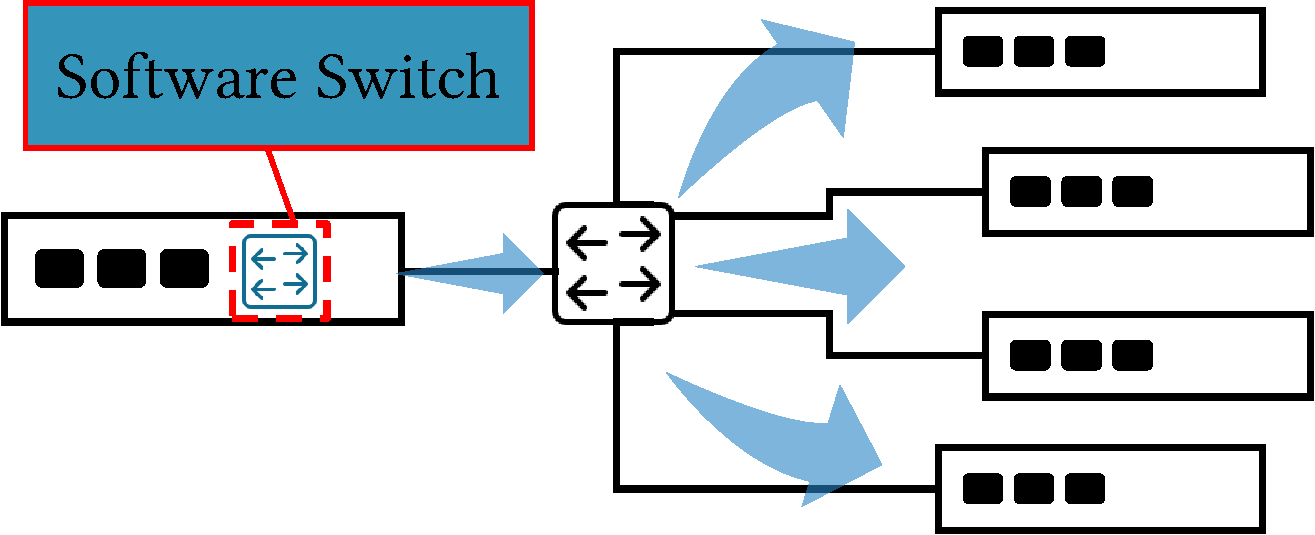
\includegraphics[width=1\linewidth]{figs/testbed2-crop.pdf}
                \vspace{-6mm}
		\caption{\small{\textit{Edge Switching}}}
                \label{fig:testbed-switching}

	\end{subfigure}
        % \rulesep
	\begin{subfigure}[t]{.46\linewidth}
		\centering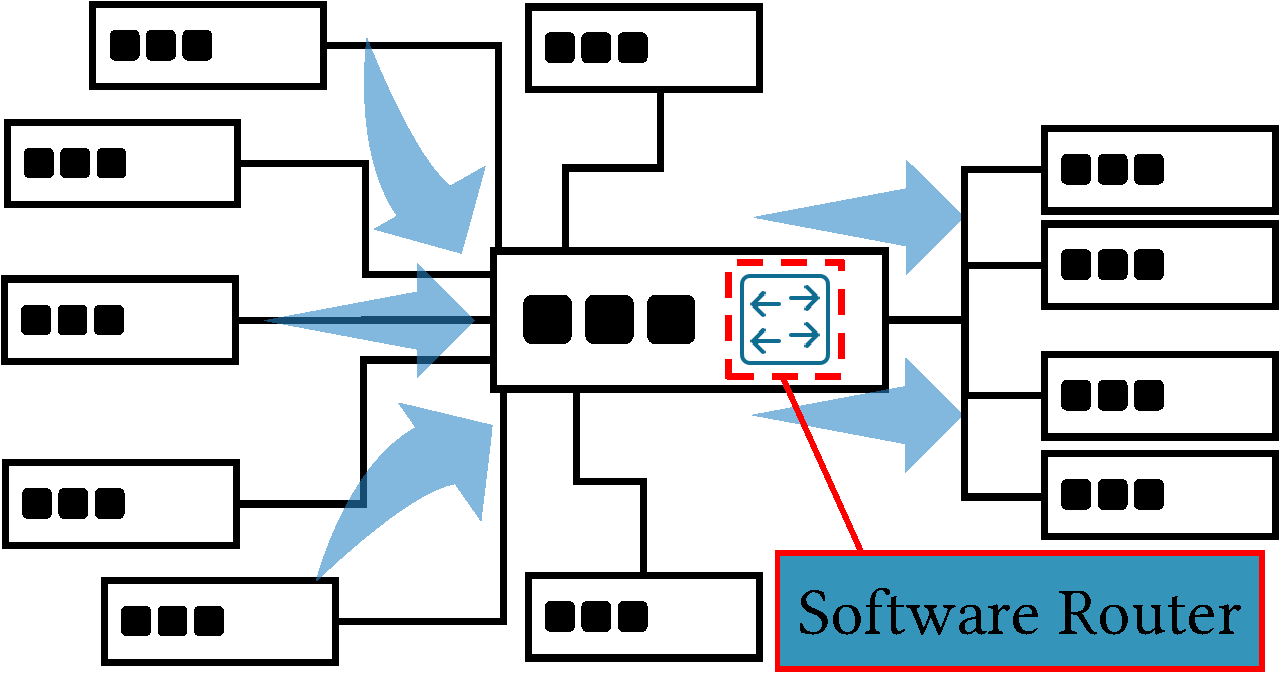
\includegraphics[width=1\linewidth]{figs/testbed1-crop.pdf}
                \vspace{-6mm}
		\caption{\small{\textit{Software Routing}}}
                \label{fig:testbed-routing}

	\end{subfigure}
        \vspace{-3mm}
	\caption{\small{
                Topologies in the physical testbed.}
	}
	\label{fig:testbed}
	\vspace*{-4mm}

	%\hspace{10pt}
\end{figure}


% \begin{table}[t]
% \caption{Parameter ranges and configurations used in the experiments.}
% \vspace{-3mm}
% \label{tab:ranges}
% \centering
% \begin{tabular}{l|l|l}
% \centering
% % \cline{1-3}
% \cellcolor[HTML]{DAE8FC}Parameter & \cellcolor[HTML]{DAE8FC}Range & \cellcolor[HTML]{DAE8FC}Default  \\
% \cellcolor[HTML]{DAE8FC}Number of Iperf flows             & 1-7168                        & 6                               \\
% \cellcolor[HTML]{DAE8FC}MTU                               & 1514-9014                     & 9014         \\          
% \cellcolor[HTML]{DAE8FC}Transport \& CC                   & TCP cubic, UDP                & cubic            \\
% \cellcolor[HTML]{DAE8FC}DRR quantum                       & 1514,9014                     & 9014        \\
% % \cellcolor[HTML]{DAE8FC}Link Speed                        & 1Gbps, 10Gbps, 25Gbps         & 10Gbps                          &  &  \\ \cline{1-3}
% \end{tabular}
% \vspace{-3mm}
% \end{table}



\subsection{Experiment Setup}
\label{sec:testbed}

We use the two topologies as depicted in Fig. \ref{fig:testbed}.  The
edge switching topology (Fig. \ref{fig:testbed-switching}) represents
packet switching on a sender host machine, for example in a virtual
switch deployed on a server in a datacenter or in the cloud. One server
acts as the traffic generator and the schedulers are configured on
that server to forward the traffic. This mimics a small-scale outcast
traffic pattern setting.
The software routing topology (Fig. \ref{fig:testbed-routing}) is used
by default and represents in-network scheduling where one software
gateway routes traffic between the senders and receivers, this
represents deployment on home routers, SD-WAN gateways, access points
or middleboxes. The schedulers are configured on the middle server to
forward the traffic between seven receiving network interfaces and one
transmitting interface being the bottleneck. This topology
enables us to emulate incast traffic patterns.
These topologies are implemented in a testbed consisting of ten Linux
servers connected via X710 10 Gbps NICs to Aruba 5406R switches.
% and via 25 Gbps links to an Intel Tofino switch. 
The scheduling server machine in the edge topology features 2x Intel
Xeon E5-2643 CPUs totaling 24 logical cores (3.4 GHz). The scheduling
server for the routing topology leverages 2x Intel Xeon E5-2680 CPUs
totaling 28 cores (2.4 GHz). A subset of our experiments is done in
a 25 Gbps topology consisting of four servers in the edge-switching
topology, connected via Intel E810 NICs and a Tofino 2 switch.
By default, each experiment runs for 1 minute. The
workload traffic is generated using versions 2.1.9 and 2.1.10 of \textit{iperf} \cite{iperf2}.
The default TCP congestion control is Cubic and we also include our test results with TCP BBRv3. The default MSS is 1456
bytes and LRO/GRO are disabled unless specified otherwise. In some
experiments, Byte Queue Limits are lowered \cite{bql}, to shrink the
NIC transmit queue and to reduce transmit batching, which can decrease
application latency.
Finally, CPU utilization is measured using Linux \textit{perf} framework \cite{linux-perf} by summing the usage of the enqueue and dequeue functions of each scheduler. 
% We also leverage \textit{pcap} hooks and \textit{Valinor} \cite{valinor} to quantify the burstiness of NIC's egress traffic.


\subsection{NIC Accelerations - TSO \& LRO}
\label{sec:scrr-eval-gsogro}

\begin{figure*}[t]
  \centering
  \begin{subfigure}[t]{.30\linewidth}
    \centering
    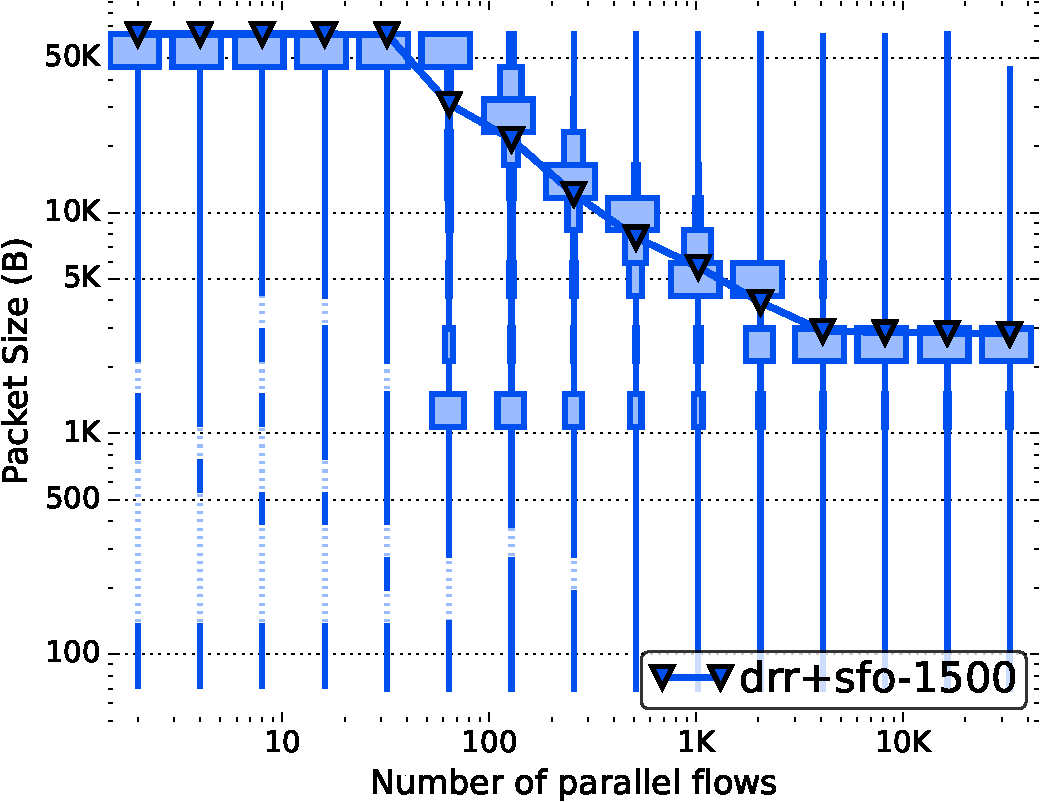
\includegraphics[width=0.95\linewidth]{figs/paral_cn_1t16x1024_gso_pkthist_fq_drr_1500.pdf}
    \caption{\small{\textit{TSO: Packet distribution}}}
    \label{fig:gso-histo-full}
  \end{subfigure}
  \begin{subfigure}[t]{.30\linewidth}
    \centering
    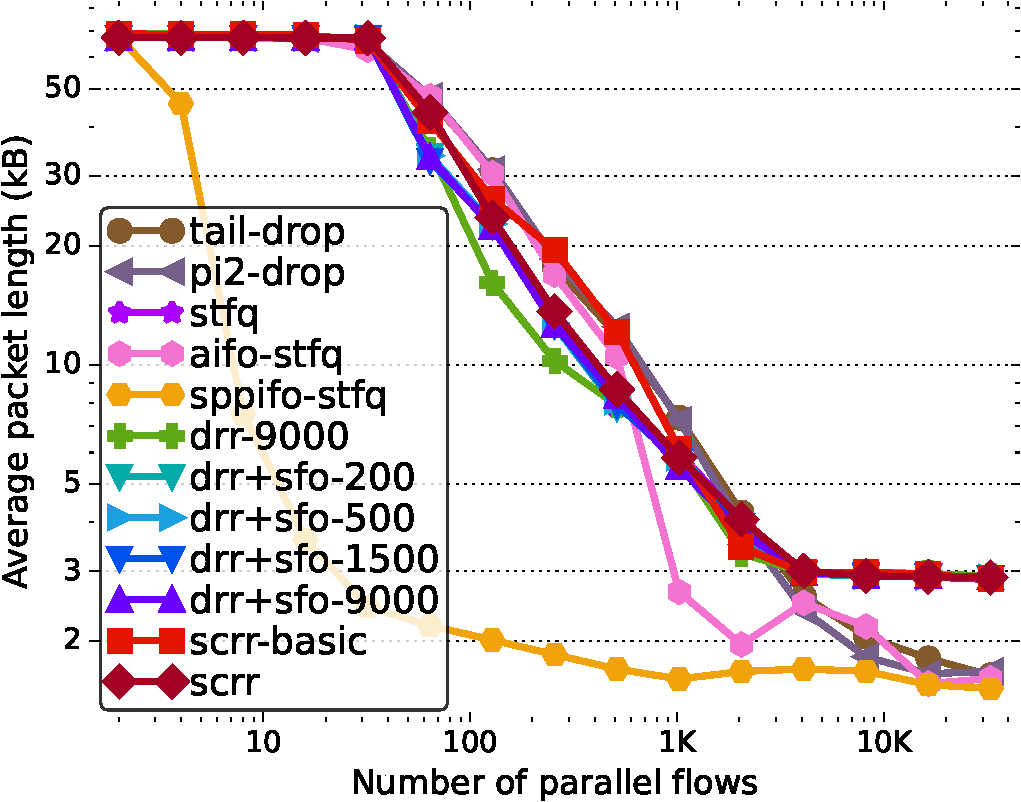
\includegraphics[width=0.95\linewidth]{figs/paral_cn_1t16x1024_gso_skblen_comp_methods.pdf}
    \caption{\small{\textit{TSO: Average packet length}}}
    \label{fig:gso-avg-full}
  \end{subfigure}
  \begin{subfigure}[t]{.30\linewidth}
    \centering
    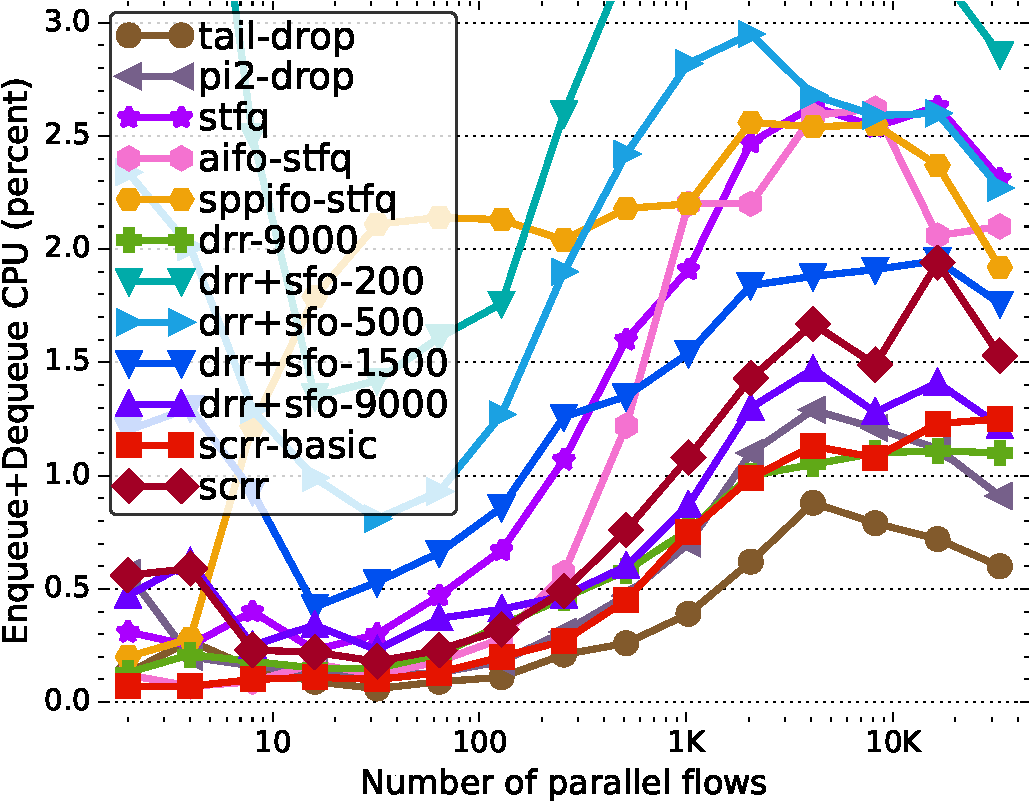
\includegraphics[width=0.95\linewidth]{figs/paral_cn_1t16x1024_gso_kp_comp_methods.pdf}
    \caption{\small{\textit{TSO: CPU overhead}}}
    \label{fig:gso-cpu-full}
  \end{subfigure}
  \\
  \begin{subfigure}[t]{.30\linewidth}
    \centering
    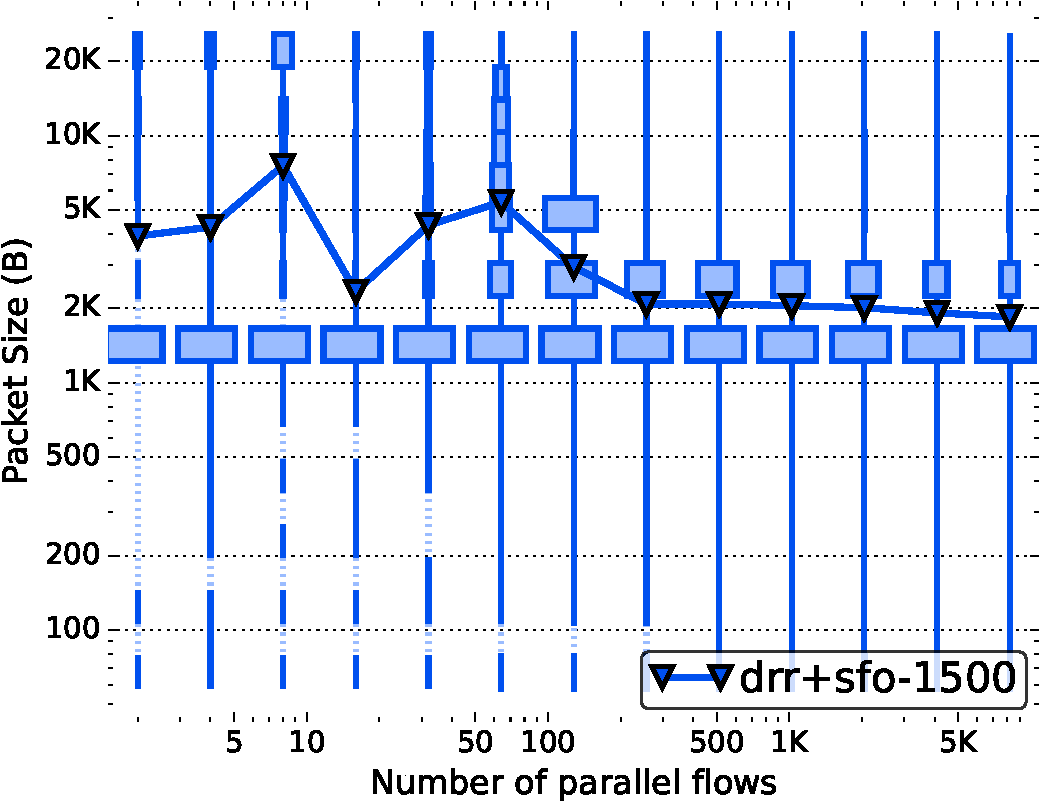
\includegraphics[width=0.95\linewidth]{figs/paral_cn_1t4x1024_gro_pkthist_fq_drr_1500.pdf}
    \caption{\small{\textit{Packet distribution}}}
    \label{fig:gro-histo-full}
  \end{subfigure}
  \begin{subfigure}[t]{.30\linewidth}
    \centering
    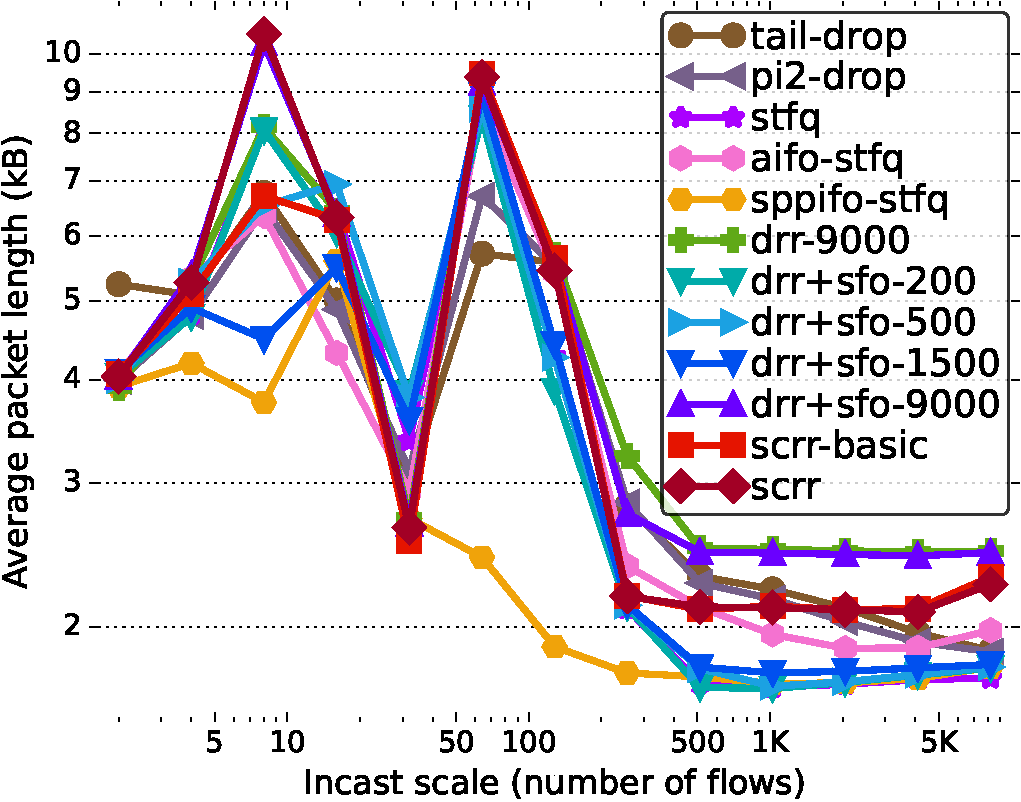
\includegraphics[width=0.95\linewidth]{figs/paral_cn_1t4x1024_gro_skblen_comp_methods.pdf}
    \caption{\small{\textit{Average packet length}}}
    \label{fig:gro-avg-full}
  \end{subfigure}
  \begin{subfigure}[t]{.30\linewidth}
    \centering
    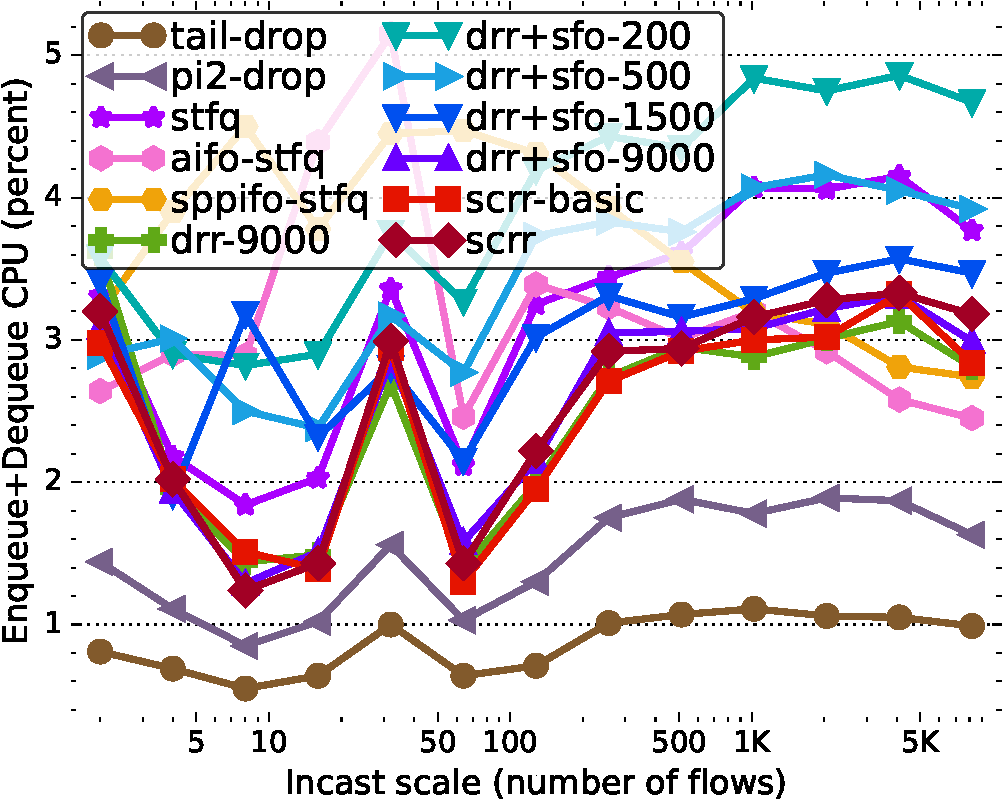
\includegraphics[width=0.95\linewidth]{figs/paral_cn_1t4x1024_gro_kp_comp_methods.pdf}
    \caption{\small{\textit{CPU overhead}}}
    \label{fig:gro-cpu-full}
  \end{subfigure}
  \vspace{-3mm}
  \caption{\small{Performance of packet schedulers under TSO (top) and LRO (bottom) accelerations.}}
  \label{fig:gsogro-full}
  \vspace{-0.2cm}
\end{figure*}



The commodity acceleration functions of modern Network Interface Cards
(NIC) are essential to sustain the high packet rates for high-speed
Ethernet in software. TCP segmentation offloading (TSO)
\cite{linux-gso-gro} and its software counterpart, Generic
Segmentation Offload (GSO), allow the sender to defer the segmentation
until the very late packet processing stages, resulting in very large
packets being passed to the qdisc. Similarly, TCP Large Receive Offload
(LRO) and its software counterpart, Generic Large Receive
Offload (GRO), allows a NIC to aggregate received packets into larger
chunks. In Linux, the current default maximum size of those packets is 64 kB and there are proposals to greatly increase this maximum
\cite{big-tcp}. This is because, a reduction in packet rate improves
software performance by reducing the overhead of context switches,
cache misses, and metadata handling. However, as studied earlier in
this work, both TSO and LRO make packet size unpredictable for
a software packet scheduler.

Figures \ref{fig:gso-histo-full} and \ref{fig:gso-avg-full} show the
impact of TSO on the packets as seen by the sender host's software
scheduler in the edge switching topology
(\ref{fig:testbed-switching}). This would be a typical packet
distribution seen in a virtual switch deployed in a datacenter or the
Cloud, or on a busy server. As the number of flows increases, the
individual bandwidth share decreases and the average TSO packet size
decreases from 64 kB to 1500B. Figure \ref{fig:gso-cpu-full} presents
the CPU overhead of the various schedulers. Smaller packets do
increase CPU overhead, as expected. This is a scenario where it is
difficult to find an optimal configuration for \textit{DRR}.
\textit{DRR-1500} is configured based on the MTU and uses a fixed
quantum of 1500B, but this causes too many CPU cycles to be wasted on
accumulating quantum over multiple scheduling rounds to send packets
that are larger than the quantum. \textit{SCRR} lowers CPU usage by
adapting to the packet sizes and has a similar CPU overhead as
\textit{DRR-9000} which uses a large quantum.

Figures \ref{fig:gro-histo-full} and \ref{fig:gro-avg-full} show LRO
packet sizes received on the router in topology
\ref{fig:testbed-routing}. This would be a typical packet distribution
seen in home routers, SD-WAN gateways, access points or
middleboxes. Two sender machines produce half of the workload flows,
so the LRO packets are aggregated on two separate NICs. The impact of
LRO is a lot less predictable than TSO, but there is still a general
trend of higher number of flows resulting in smaller packet sizes. DRR
with smaller quantum cannot adapt to the dynamics of the traffic,
causing CPU wastage. Again, \textit{SCRR} lowers CPU usage by adapting
to the packet sizes and has a similar CPU overhead as
\textit{DRR-9000} which uses a large quantum.

The default quantum of the Linux 'sch\_fq' module is 3000B
\cite{sch-fq}, i.e., 2$\times$ the MTU. From the packet distributions
in Figures \ref{fig:gso-histo-full} and \ref{fig:gro-histo-full}, it's
a logical choice as it's a very common packet size, and would allow to
send most packets without the need to accumulate deficit for LRO and
TSO with high number of flows.




\subsection{Impact of CPU overhead on throughput}
\label{app:eval-fairness}

CPU utilization is a good proxy for the overall resource
requirements of the packet scheduler. Some software implementations of
packet schedulers in Internet gateways result in reduced network
throughput due to their high CPU usage \cite{cake-perf1,
  cake-perf2}. It is usually tricky to estimate the impact of such CPU
overhead, because different packet schedulers may interract
differently with the rest of the networking stack. By changing the
quantum of DRR, we can artificially increase the CPU overhead of
packet scheduling without changing anything else, and isolate the
contribution of the packet scheduler overhead. When the quanta is
below 1000~B, packets are scheduled in the exact same
order. Experiments in Fig. \ref{fig:cpu-drr-quantum} create an incast
of heavy flows sharing a bottleneck link serviced by \textit{DRR}, and
the CPU overhead increased by reducing the quantum.


Figure \ref{fig:cpu-quanta-tcp-lat-10f} shows the CPU overhead of the
packet scheduler and the throughput when using TCP flows.  Each of the
7 sender generates 10 flows and each uses a MSS of 1000, 1500, 2000,
3000, 5000, 7000 and 8956~bytes respectively. At higher quanta, the
lower per-packet processing time is balanced by the increasing packet
rate, and CPU usage is constant. A small 100B quantum makes
\textit{DRR} the bottleneck and reduces aggregate throughput to
5~Gb/s, which is a third of the capacity. The CPU usage for
\textit{DRR} is less than 7\%, however this puts enough pressure on
the rest of the networking stack to cause such a slowdown.


Figure \ref{fig:cpu-quanta-tcp-lat-100f} reproduce and extend this
experiment on our new testbed. Each of the 7 sender generates 100
flows and each uses a MSS of 1500, 2000, 3000, 4000, 6000, 8000 and
8956~bytes respectively. The frequency of the CPU was downscaled to
1~GHz to mimic the original testbed. The performance of \textit{DRR}
is similar to the experiment on the original testbed in
Figure \ref{fig:cpu-quanta-tcp-lat-10f}. \textit{SCRR} achieve optimal
throughput, however a smaller set of packets would cause both
\textit{SCRR} and \textit{DRR} to have lower throughput. \textit{SCRR}
achieve low throughput because every iteration of the dequeue function
is guaranteed to dequeue a packet.

\begin{figure*}[th!]
  \centering
  \begin{subfigure}[t]{.30\linewidth}
    \centering
    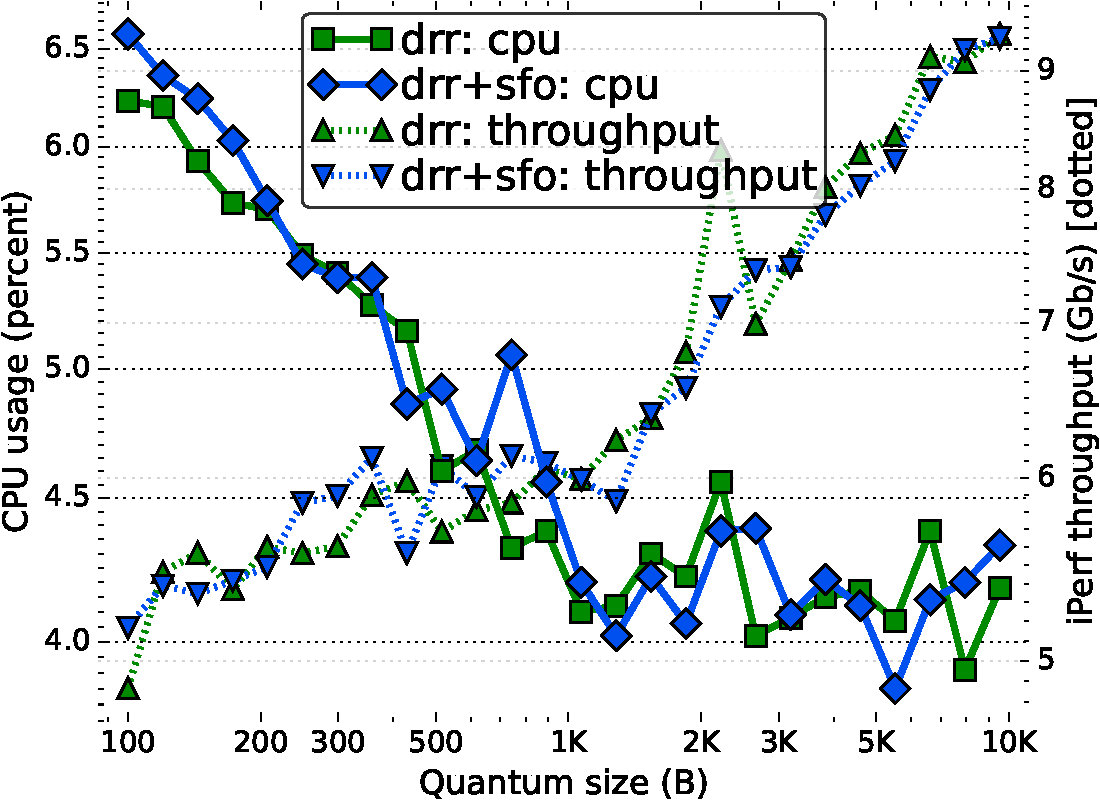
\includegraphics[width=0.95\linewidth]{figs/burst_cn_6t1x10_mss_1000_kp_bw_drr_basic_fq_drr.pdf}
    \caption{\small{\textit{CPU vs TCP throughput, 70 flows}}}
    \label{fig:cpu-quanta-tcp-lat-10f}
  \end{subfigure}
  \begin{subfigure}[t]{.30\linewidth}
    \centering
    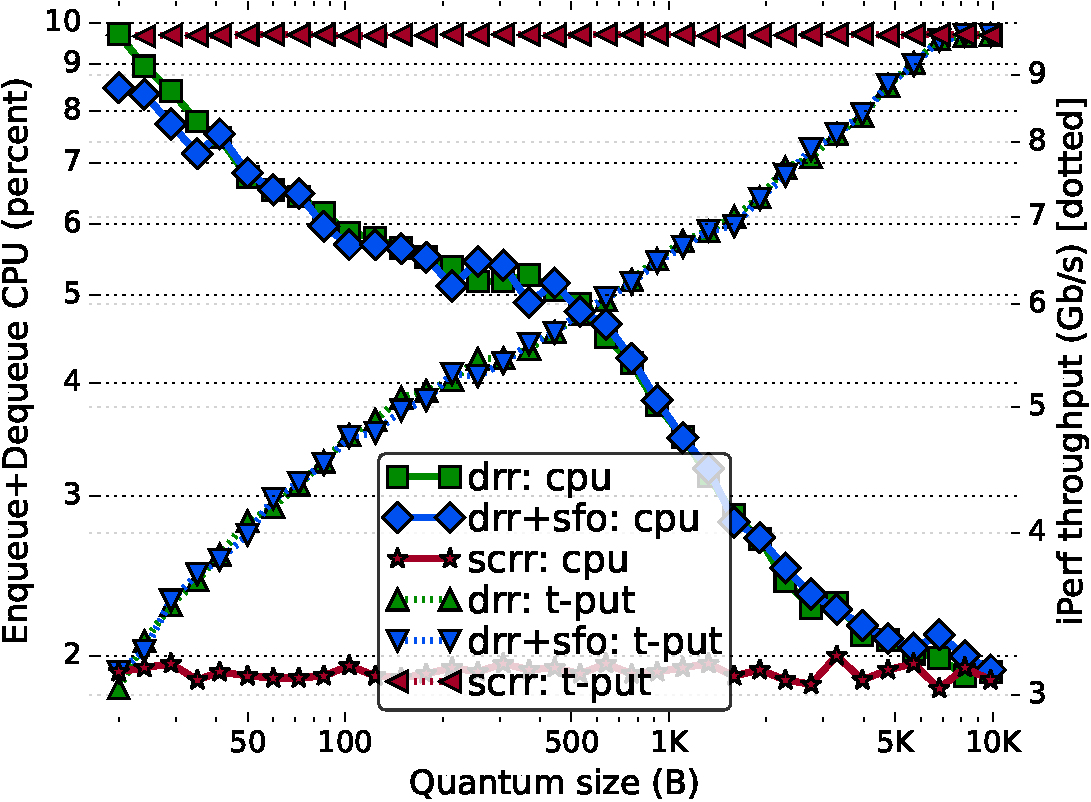
\includegraphics[width=0.95\linewidth]{figs/burst_cn_6t1x100_kp_bw_drr_basic_fq_drr_scrr-neia.pdf}
    \caption{\small{\textit{CPU vs TCP throughput, 700 flows}}}
    \label{fig:cpu-quanta-tcp-lat-100f}
  \end{subfigure}
  \begin{subfigure}[t]{.30\linewidth}
    \centering
    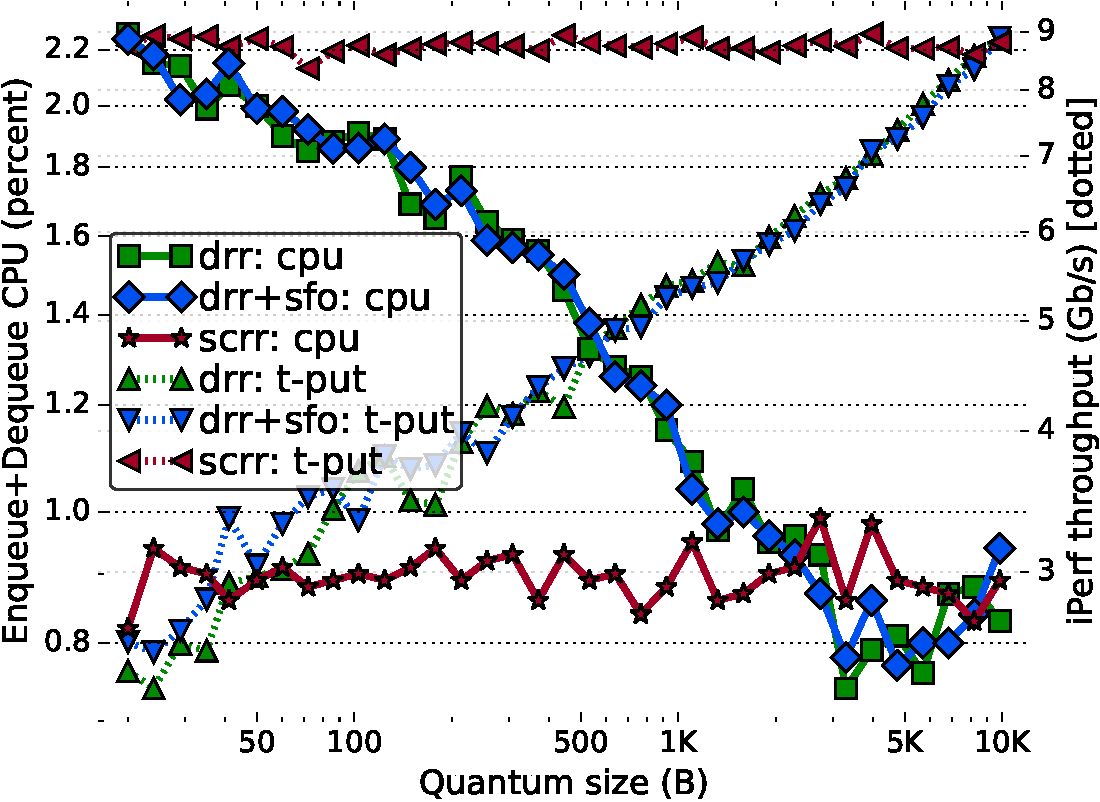
\includegraphics[width=0.95\linewidth]{figs/burst_cn_6u1x100_Cb_2G_kp_bw_drr_basic_fq_drr_scrr-neia.pdf}
    \caption{\small{\textit{CPU vs UDP throughput, 700 flows}}}
    \label{fig:cpu-quanta-udp-lat-100f}
  \end{subfigure}
  \\
  \begin{subfigure}[t]{\linewidth}
    \centering
    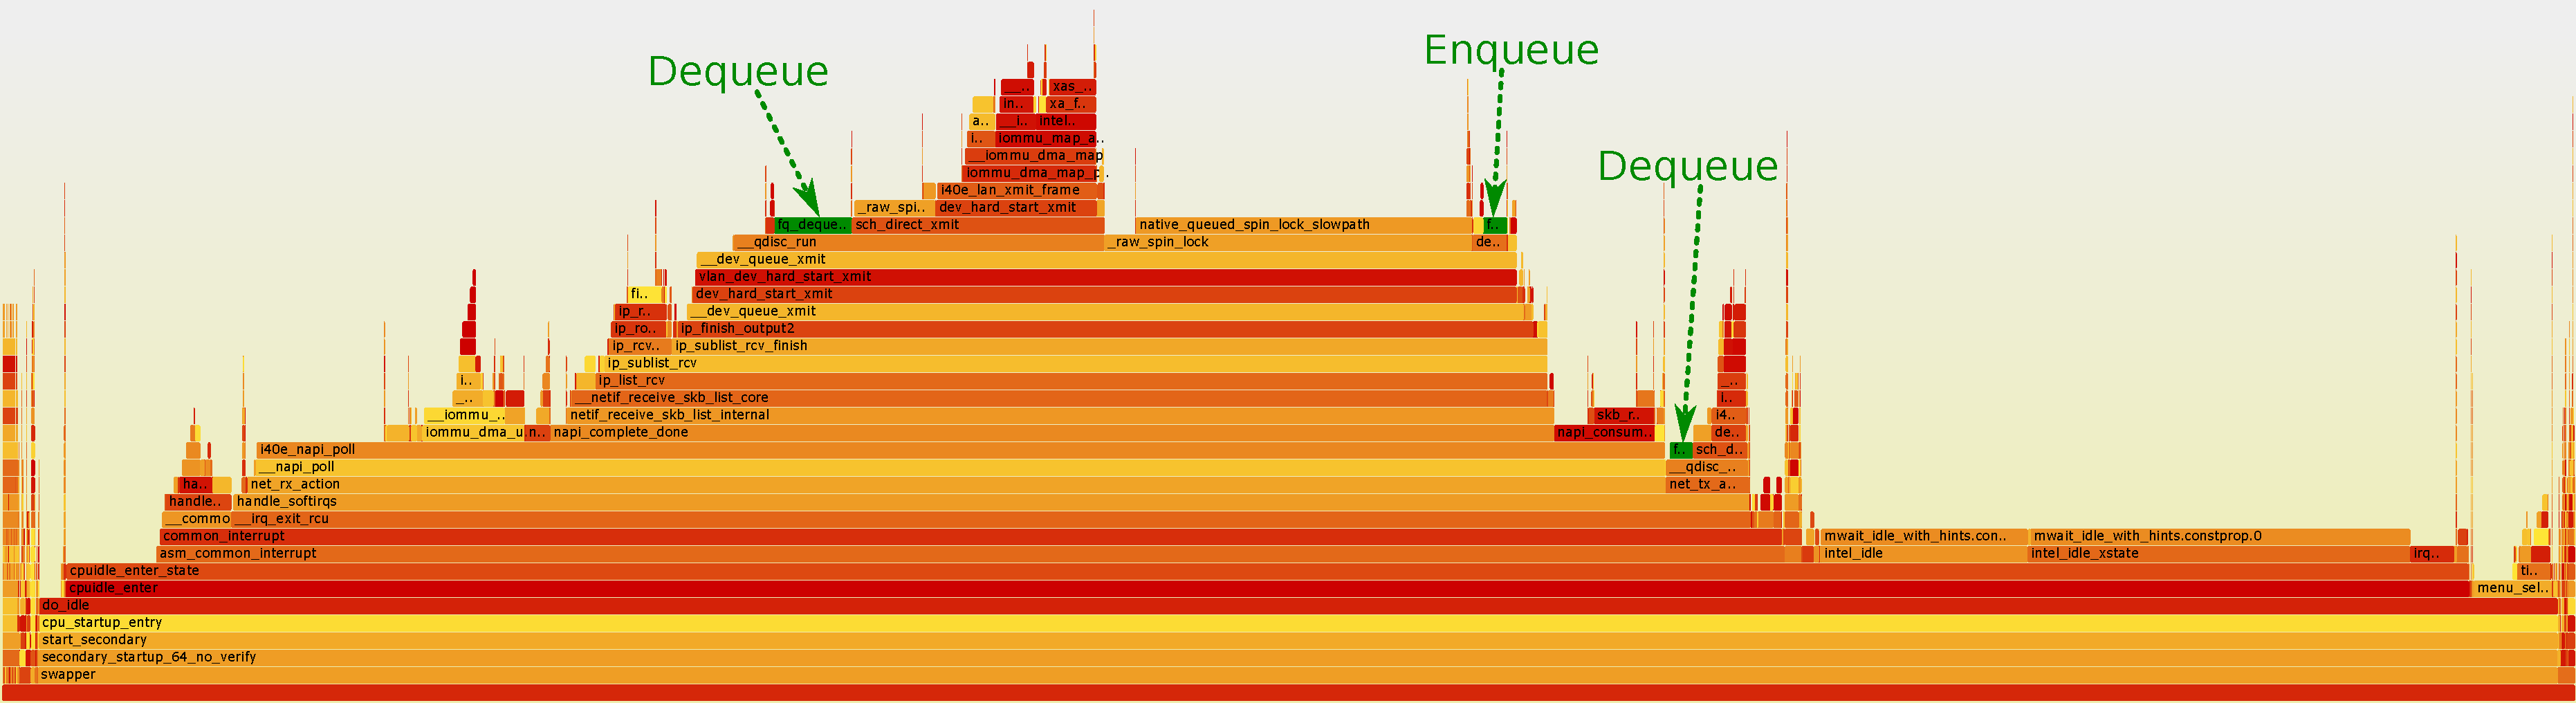
\includegraphics[width=0.95\linewidth]{figs/burst_cn_6t1x100_flame_drr_basic.pdf}
    \caption{\small{\textit{FlameGraph, TCP, Quantum 500~B}}}
    \label{fig:cpu-quanta-tcp-flamegraph}
  \end{subfigure}
  \vspace{-3mm}
  \caption{\small{Impact DRR quantum on CPU overhead and traffic throughput.}}
  \vspace{-0.4cm}
  \label{fig:cpu-drr-quantum}
\end{figure*}



Figure \ref{fig:cpu-quanta-udp-lat-100f} repeats the experiment of
Figure \ref{fig:cpu-quanta-tcp-lat-100f} using UDP flows, the flows are
constant bit rate and the aggregate rate per sender is 2~Gb/s, for
a total of 14~Gb/s. The result is broadly similar to the experiment
with TCP flows, however the CPU overhead measured is much lower. Also,
with the highest quantum, CPU overhead goes up. We do not have a good
explanation for those results, however, the Linux network stack is
complex, and cache performance impact can be unintuitive. With UDP
traffic, the networking stack has to process a lot more packets and
drop them, which might be the cause of that difference. The ratio of
packet drops (not shown) is the inverse mirror of the throughput, the
sending rate is constant, so a lower throughput means more packets are
dropped.

Figure \ref{fig:cpu-quanta-tcp-flamegraph} shows the detail of the CPU overhead
of the various kernel functions as a FlameGraph for the experiment in
Figure \ref{fig:cpu-quanta-tcp-lat-100f} with quantum size 500~B. During
packet processing many other parts of the Linux network stack must be
exercised that respectively consume CPU. With more pressure on the
qdisc, the network stack processing also experiences more CPU
contention and cache pressure. As expected, the dequeue operation
consume more CPU, because it needs to spin to accumulate quanta for
each flow. Figure \ref{fig:cpu-gro-eqdq} presents the CPU overhead of the
enqueue and dequeue function in a different type of experiment.

\begin{figure}[th!]
  \centering
  \begin{subfigure}[t]{.30\linewidth}
    \centering
    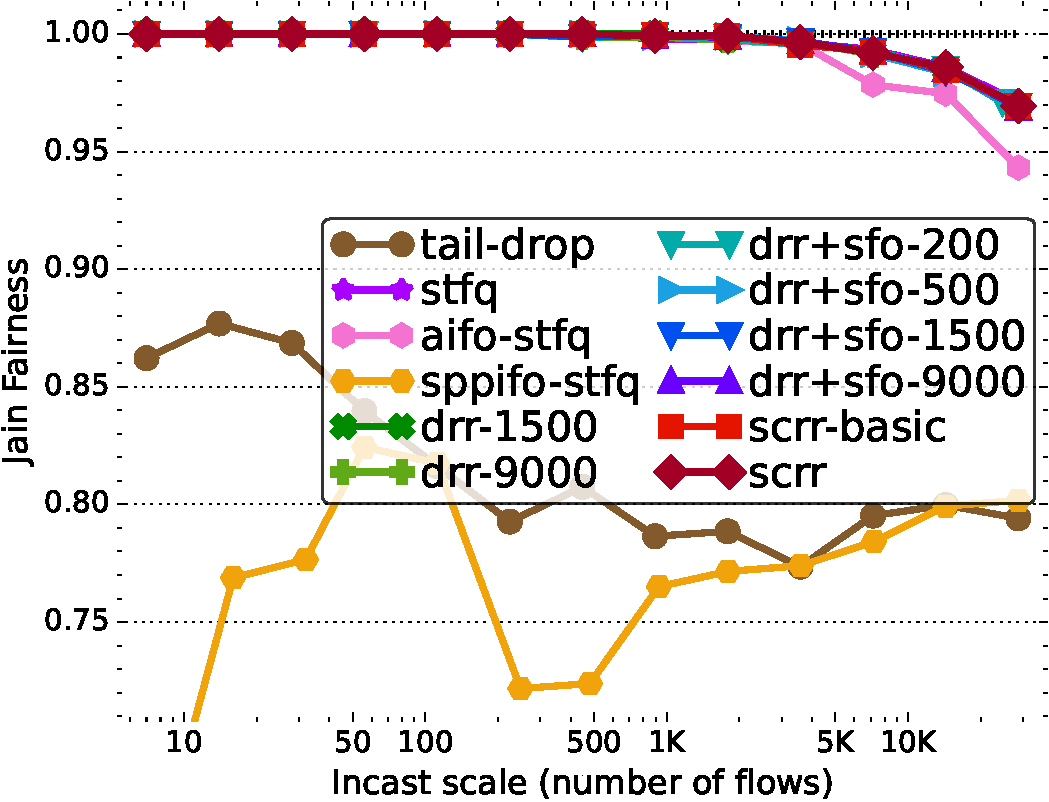
\includegraphics[width=0.95\linewidth]{figs/paral_cn_6u4x1024_Cb_7G_jain_comp_methods.pdf}
    \caption{UDP-rate: Jain}
    \label{fig:fairness-jain-udp-rate-full}
  \end{subfigure}
  \begin{subfigure}[t]{.30\linewidth}
    \centering
    \includegraphics[width=0.95\linewidth]{figs/paral_cn_6u4x1024_mss_2500_jain_comp_methods.pdf}
    \caption{UDP-MSS: Jain}
    \label{fig:fairness-jain-udp-mss-full}
  \end{subfigure}
  \begin{subfigure}[t]{.30\linewidth}
    \centering
    \includegraphics[width=0.95\linewidth]{figs/paral_cn_6t4x1024_mss_2500_jain_comp_methods.pdf}
    \caption{TCP-MSS: Jain}
    \label{fig:fairness-jain-tcp-mss-full}
  \end{subfigure}
  \\
  \begin{subfigure}[t]{.30\linewidth}
    \centering
    \includegraphics[width=0.95\linewidth]{figs/paral_cn_6u4x1024_Cb_7G_bw_comp_methods.pdf}
    \caption{UDP-rate: Throughput}
    \label{fig:fairness-tput-udp-rate-full}
  \end{subfigure}
  \begin{subfigure}[t]{.30\linewidth}
    \centering
    \includegraphics[width=0.95\linewidth]{figs/paral_cn_6u4x1024_mss_2500_bw_comp_methods.pdf}
    \caption{UDP-MSS: Throughput}
    \label{fig:fairness-tput-udp-mss-full}
  \end{subfigure}
  \begin{subfigure}[t]{.30\linewidth}
    \centering
    \includegraphics[width=0.95\linewidth]{figs/paral_cn_6t4x1024_mss_2500_bw_comp_methods.pdf}
    \caption{TCP-MSS bias: Throughput}
    \label{fig:fairness-tput-tcp-mss-full}
  \end{subfigure}
  \\
  \begin{subfigure}[t]{.30\linewidth}
    \centering
    \includegraphics[width=0.95\linewidth]{figs/paral_cn_6u4x1024_Cb_7G_kp_comp_methods.pdf}
    \caption{UDP-rate bias: CPU}
    \label{fig:fairness-cpu-udp-rate-full}
  \end{subfigure}
  \begin{subfigure}[t]{.30\linewidth}
    \centering
    \includegraphics[width=0.95\linewidth]{figs/paral_cn_6u4x1024_mss_2500_kp_comp_methods.pdf}
    \caption{UDP-MSS: CPU}
    \label{fig:fairness-cpu-udp-mss-full}
  \end{subfigure}
  \begin{subfigure}[t]{.30\linewidth}
    \centering
    \includegraphics[width=0.95\linewidth]{figs/paral_cn_6t4x1024_mss_2500_kp_comp_methods.pdf}
    \caption{TCP-MSS: CPU}
    \label{fig:fairness-cpu-tcp-mss-full}
  \end{subfigure}
  \vspace{-3mm}
  \caption{\small{Fairness of packet schedulers and their CPU overhead as the scale of Incast increases under two different biases: rate and MSS.}}
  \label{fig:fairness-full}
  \vspace{-0.2cm}
\end{figure}



\subsection{Fairness Under Different Biases}
\label{sec:scrr-eval-fairness}

The crucial property of a packet scheduler is enforcing fairness and
QoS. To better scale the
experiments, we configured all scheduling classes with identical
weights and configured various biases between flows to create
potential unfairness. These experiments showcase how the scheduler
achieves fairness by overcoming these biases.

The first bias we introduce is the rate at which flows arrive at the
scheduler. This is a much-generalized version of the experiments in
previous papers \cite{drr}, where it aims to investigate how well
a scheduler deals with incast traffic and a large number of
misbehaving flows. The testbed is the original testbed
(\S\ref{sec:testbed}) and we are using the routing topology
\ref{fig:testbed-routing}. The seven senders generate UDP traffic,
each with different aggregate offered rates of 1.5, 2, 3, 4, 5, 6, and
7~Gb/s, respectively. The number of UDP connections per sender varies
from 1 to 4096, for a maximum of 28672
flows. Figure \ref{fig:fairness-jain-udp-rate-full} depicts the Jain
Index measuring fairness across the flows. The \textit{tail-drop} and
\textit{SP-PIFO} schedulers show poor fairness since it admits packets
proportional to their arrival rate, favoring UDP flows with higher
rates. All fair queueing schedulers, including \textit{SCRR}, have
excellent fairness, as expected, as they enforce byte-level fairness
for every flow. At a very high number of UDP flows (28k), the fairness
of all schedulers is impacted by hash collisions in the classifier,
a well-known caveat of using hashing in flow classifiers. Most QoS
classifiers have well-defined QoS classes that do not use hashing, and
would not suffer from this issue.

Figure \ref{fig:fairness-tput-udp-rate-full} presents the aggregate
throughput of the UDP flows. \textit{DRR-200} and \textit{DRR-500} are
methods that waste CPU cycles (\S\ref{sec:drr-tradeoff}) and they result in decreased throughput at higher flow counts. This is because an increase in flow count increases the cache footprint of the scheduler and the probability of cache
misses. Figure \ref{fig:fairness-cpu-udp-rate-full} presents the CPU
overhead on the router. In general, a higher CPU overhead is more
likely to impact throughput (\S\ref{sec:drr-tradeoff}), however, in
this experiment, the relation between the two is not obvious. We
believe that the need to drop a very large number of packets distorts
the CPU overhead numbers measured. A lower quantum increases CPU
consumption for \textit{DRR}, as more scheduling cycles are needed to
accumulate enough quantum. All variants of \textit{SCRR} offer lower
CPU utilization amongst the schedulers.

The second bias we introduce is the packet size. Varying the packet
sizes forces the schedulers to transmit more packets from flows that
send smaller packets in order to satisfy the proper byte-level
accounting of the schedulers. The seven sender machines generate UDP
traffic, each using a different Maximum Segment Size of 2500, 3000,
3500, 5000, 6000, 8500, and 8956 bytes,
respectively. Figure \ref{fig:fairness-jain-udp-mss-full} shows the Jain
Index measuring fairness across the flows. The \textit{tail-drop}
queue yields poor fairness again. This is because the incast traffic
causes the single FIFO to always be at its peak utilization. In this
state, it becomes more probable for the queue to have enough space for
small packets under the byte limit (18 MB, or 15 ms of traffic), which
further favors flows with small packets. All other schedulers have
excellent fairness, as
expected. Figure \ref{fig:fairness-tput-udp-mss-full} shows the
aggregate throughput of the UDP flows, again \textit{DRR-200} and
\textit{DRR-500} show reduced
throughput. Figure \ref{fig:fairness-cpu-udp-mss-full} shows the CPU
overhead on the router, asserting \textit{SCRR}'s low CPU overhead.

The packet size bias can also be used for TCP
traffic. Figure \ref{fig:fairness-jain-tcp-mss-full} plots the Jain
Index for TCP Cubic flows. At a very high number of TCP flows (28k),
some flows experience reduced performance or stalls, especially with
schedulers that use the \textit{tail-drop} queue. The TCP congestion
protocol is not designed to provide byte-level fairness, therefore
\textit{tail-drop} shows only slightly better fairness compared to
UDP. However, this time, flows with larger packets are favored. In the
congestion avoidance phase, TCP increases the congestion window by one
whole packet for each RTT, therefore flows with larger packets can
increase their throughput faster. The \textit{PI2} AQM is not designed
for byte-level fairness either, which explains why it performs
similarly to \textit{tail-drop}. The same applies to \textit{AIFO} and
\textit{SP-PIFO}. All fair schedulers provide superior fairness as
they enforce byte-level fairness among
classes. Figure \ref{fig:fairness-tput-udp-mss-full} shows the aggregate
throughput of the TCP flows. The TCP flows are much more impacted than
UDP flows, as packet drops cause the congestion control to reduce the
congestion window. Figure \ref{fig:fairness-cpu-tcp-mss-full} shows the
CPU overhead on the router. In this experiment, the throughput
decrease can be directly correlated with the CPU overhead. As
expected, the schedulers consume more CPU than the \textit{tail-drop}
and \textit{PI2}, and as in previous experiments, the \textit{SCRR}
variants are among the schedulers with the lowest overhead.

\begin{figure*}[th!]
  \centering
  \begin{subfigure}[t]{.30\linewidth}
    \centering
    \includegraphics[width=0.95\linewidth]{figs/pkt_size_cn_2t4x8_mn_2tb2x4_per_15_mss_1468_lat_comp_drr-200_scrr.pdf}
    \caption{\small{\textit{Router: Varying Response Size, Latency}}}
    \label{fig:reply-1456-latency-sched-full}
  \end{subfigure}
  \begin{subfigure}[t]{.30\linewidth}
    \centering
    \includegraphics[width=0.95\linewidth]{figs/pkt_size_edge_cn_2t1x32_mn_2tb1x8_mss_1468_lat_comp_schys_drr_scrr.pdf}
    \caption{\small{\textit{Edge: Varying Request Size, Latency}}}
    \label{fig:request-edge-1456-latency-sched-full}
  \end{subfigure}
  %\begin{subfigure}[t]{.30\linewidth}
  %  \centering
  %  \includegraphics[width=0.95\linewidth]{figs/pkt_size_cn_2t4x8_mn_2tb2x4_mss_1468_lat_comp_drr_scrr.pdf}
  %  \caption{\small{\textit{Router: Varying Request Size, Latency}}}
  %  \label{fig:request-1456-latency-sched-full}
  %\end{subfigure}
  \begin{subfigure}[t]{.30\linewidth}
    \centering
    \includegraphics[width=0.95\linewidth]{figs/pkt_size_cn_2t4x16_mn_2ui32_mss_1468_lat_comp_drr_scrr.pdf}
    \caption{\small{\textit{Router: Varying VBR packet size, Latency}}}
    \label{fig:vbr-1456-latency-sched-full}
  \end{subfigure}
  \\
  \begin{subfigure}[t]{.30\linewidth}
    \centering
    \includegraphics[width=0.95\linewidth]{figs/pkt_size_cn_2t4x8_mn_2tb2x4_per_15_mss_1468_kp_comp_methods.pdf}
    \caption{\small{\textit{Router: Varying Response Size, CPU}}}
    \label{fig:reply-1456-cpu-full}
  \end{subfigure}
  \begin{subfigure}[t]{.30\linewidth}
    \centering
    \includegraphics[width=0.95\linewidth]{figs/pkt_size_edge_cn_2t1x32_mn_2tb1x8_mss_1468_kp_comp_methods.pdf}
    \caption{\small{\textit{Edge: Varying Request Size, CPU}}}
    \label{fig:request-edge-1456-cpu-full}
  \end{subfigure}
  %\begin{subfigure}[t]{.30\linewidth}
  %  \centering
  %  \includegraphics[width=0.95\linewidth]{figs/pkt_size_cn_2t4x8_mn_2tb2x4_mss_1468_kp_comp_methods.pdf}
  %  \caption{\small{\textit{Router: Varying Request Size, CPU}}}
  %  \label{fig:request-1456-cpu-full}
  %\end{subfigure}
  \begin{subfigure}[t]{.30\linewidth}
    \centering
    \includegraphics[width=0.95\linewidth]{figs/pkt_size_cn_2t4x16_mn_2ui32_mss_1468_kp_comp_methods.pdf}
    \caption{\small{\textit{Router: Varying VBR packet size, CPU}}}
    \label{fig:vbr-1456-cpu-full}
  \end{subfigure}
  \\
  \begin{subfigure}[t]{.30\linewidth}
    \centering
    \includegraphics[width=0.95\linewidth]{figs/burst_cn_2t4x8_mn_2tb2x4_crs_500_kp_lat_drr_basic_fq_drr.pdf}
    \caption{\small{\textit{Router: Varying Response Size, DRR+SFO at 500B}}}
    \label{fig:reply-1456-drr-full}
  \end{subfigure}
  \begin{subfigure}[t]{.30\linewidth}
    \centering
    \includegraphics[width=0.95\linewidth]{figs/burst_edge_cn_2t1x32_mn_2tb1x8_mss_1468_kp_lat_drr_basic_fq_drr.pdf}
    \caption{\small{\textit{Edge: Varying Request Size, DRR+SFO at 500B}}}
    \label{fig:request-edge-1456-drr-full}
  \end{subfigure}
  %\begin{subfigure}[t]{.30\linewidth}
  %  \centering
  %  \includegraphics[width=0.95\linewidth]{figs/burst_cn_2t4x8_mn_2tb2x4_css_500_kp_lat_fq_drr.pdf}
  %  \caption{\small{\textit{Router: Varying Request Size, DRR+SFO at 500B}}}
  %  \label{fig:request-1456-drr-full}
  %\end{subfigure}
  \begin{subfigure}[t]{.30\linewidth}
    \centering
    \includegraphics[width=0.95\linewidth]{figs/burst_cn_2t4x16_mn_2ui32_css_500_kp_lat_drr_basic_fq_drr.pdf}
    \caption{\small{\textit{Router: Varying VBR packet size, DRR+SFO at 500B}}}
    \label{fig:vbr-1456-drr-full}
  \end{subfigure}
  \\
  \begin{subfigure}[t]{.30\linewidth}
    \centering
    \includegraphics[width=0.95\linewidth]{figs/pkt_size_cn_2t4x8_mn_2tb2x4_per_15_mss_1468_kp_lat_comp_methods.pdf}
    \caption{\small{\textit{Router: Varying Response Size}}}
    \label{fig:reply-1456-cpu-latency-full}
  \end{subfigure}
  \begin{subfigure}[t]{.30\linewidth}
    \centering
    \includegraphics[width=0.95\linewidth]{figs/pkt_size_edge_cn_2t1x32_mn_2tb1x8_mss_1468_kp_lat_comp_methods.pdf}
    \caption{\small{\textit{Edge: Varying Request Size}}}
    \label{fig:request-edge-1456-cpu-latency-full}
  \end{subfigure}
  %\begin{subfigure}[t]{.30\linewidth}
  %  \centering
  %  \includegraphics[width=0.95\linewidth]{figs/pkt_size_cn_2t4x8_mn_2tb2x4_mss_1468_kp_lat_comp_methods.pdf}
  %  \caption{\small{\textit{Router: Varying Request Size}}}
  %  \label{fig:request-1456-cpu-latency-full}
  %\end{subfigure}
  \begin{subfigure}[t]{.30\linewidth}
    \centering
    \includegraphics[width=0.95\linewidth]{figs/pkt_size_cn_2t4x16_mn_2ui32_mss_1468_kp_lat_comp_methods.pdf}
    \caption{\small{\textit{Router: Varying VBR packet size}}}
    \label{fig:vbr-1456-cpu-latency-full}
  \end{subfigure}
  \vspace{-3mm}
  \caption{\small{Impact of packet  schedulers on application response times for latency sensitive workloads with Cubic transport.}}
  \vspace{-0.4cm}
  \label{fig:request-full}
\end{figure*}


%\begin{figure*}[t]
%  \centering
%  \begin{subfigure}[t]{.24\linewidth}
%    \centering
%    \includegraphics[width=0.95\linewidth]{figs/pkt_size_cn_2t4x8_mn_2tb2x4_mss_1468_lat_comp_drr_scrr.pdf}
%    \caption{\small{\textit{MSS 1456B: Latency}}}
%    \label{fig:request-1456-latency-sched-full}
%  \end{subfigure}
%  \begin{subfigure}[t]{.24\linewidth}
%    \centering
%    \includegraphics[width=0.95\linewidth]{figs/pkt_size_cn_2t4x8_mn_2tb2x4_mss_1468_kp_comp_methods.pdf}
%    \caption{\small{\textit{MSS 1456B: CPU}}}
%    \label{fig:request-1456-cpu-full}
%  \end{subfigure}
%  \begin{subfigure}[t]{.24\linewidth}
%    \centering
%    \includegraphics[width=0.95\linewidth]{figs/burst_cn_2t4x8_mn_2tb2x4_css_500_kp_lat_fq_drr.pdf}
%    \caption{\small{\textit{MSS 1456B: DRR at 500B}}}
%    \label{fig:request-1456-drr-full}
%  \end{subfigure}
%  \begin{subfigure}[t]{.24\linewidth}
%    \centering
%    \includegraphics[width=0.95\linewidth]{figs/pkt_size_cn_2t4x8_mn_2tb2x4_mss_1468_kp_lat_comp_methods.pdf}
%    \caption{\small{\textit{MSS 1456B: CPU vs. latency}}}
%    \label{fig:request-1456-cpu-latency-full}
%  \end{subfigure}
%  \\
%  \begin{subfigure}[t]{.24\linewidth}
%    \centering
%    \includegraphics[width=0.95\linewidth]{figs/pkt_size_cn_2t4x8_mn_2tb2x4_mss_8956_lat_comp_drr_scrr.pdf}
%    \caption{\small{\textit{MSS 8956B: Latency}}}
%    \label{fig:request-8956-latency-sched-full}
%  \end{subfigure}
%  \begin{subfigure}[t]{.24\linewidth}
%    \centering
%    \includegraphics[width=0.95\linewidth]{figs/pkt_size_cn_2t4x8_mn_2tb2x4_mss_8956_kp_comp_methods.pdf}
%    \caption{\small{\textit{MSS 8956B: CPU}}}
%    \label{fig:request-8956-cpu-full}
%  \end{subfigure}
%  \begin{subfigure}[t]{.24\linewidth}
%    \centering
%    \includegraphics[width=0.95\linewidth]{figs/burst_cn_2t4x8_mn_2tb2x4_mss_8956_kp_lat_fq_drr.pdf}
%    \caption{\small{\textit{MSS 8956B: DRR at 500B}}}
%    \label{fig:request-8956-drr-full}
%  \end{subfigure}
%  \begin{subfigure}[t]{.24\linewidth}
%    \centering
%    \includegraphics[width=0.95\linewidth]{figs/pkt_size_cn_2t4x8_mn_2tb2x4_mss_8956_kp_lat_comp_methods.pdf}
%    \caption{\small{\textit{MSS 8956B: CPU vs. latency}}}
%    \label{fig:request-8956-cpu-latency-full}
%  \end{subfigure}
%  \vspace{-3mm}
%  \caption{\small{\textit{Impact of packet  schedulers on request latency}}}
%  \vspace{-0.4cm}
%  \label{fig:request-full}
%\end{figure*}


\subsection{Application Performance Under TCP Cubic}
\label{sec:scrr-eval-latency}
\label{sec:scrr-eval-streaming}
%\begin{figure*}[th!]
  \centering
  \begin{subfigure}[t]{.30\linewidth}
    \centering
    \includegraphics[width=0.95\linewidth]{figs/pkt_size_cn_2t4x8_mn_2tb2x4_per_15_mss_1468_lat_comp_drr-200_scrr.pdf}
    \caption{\small{\textit{Router: Varying Response Size, Latency}}}
    \label{fig:reply-1456-latency-sched-full}
  \end{subfigure}
  \begin{subfigure}[t]{.30\linewidth}
    \centering
    \includegraphics[width=0.95\linewidth]{figs/pkt_size_edge_cn_2t1x32_mn_2tb1x8_mss_1468_lat_comp_schys_drr_scrr.pdf}
    \caption{\small{\textit{Edge: Varying Request Size, Latency}}}
    \label{fig:request-edge-1456-latency-sched-full}
  \end{subfigure}
  %\begin{subfigure}[t]{.30\linewidth}
  %  \centering
  %  \includegraphics[width=0.95\linewidth]{figs/pkt_size_cn_2t4x8_mn_2tb2x4_mss_1468_lat_comp_drr_scrr.pdf}
  %  \caption{\small{\textit{Router: Varying Request Size, Latency}}}
  %  \label{fig:request-1456-latency-sched-full}
  %\end{subfigure}
  \begin{subfigure}[t]{.30\linewidth}
    \centering
    \includegraphics[width=0.95\linewidth]{figs/pkt_size_cn_2t4x16_mn_2ui32_mss_1468_lat_comp_drr_scrr.pdf}
    \caption{\small{\textit{Router: Varying VBR packet size, Latency}}}
    \label{fig:vbr-1456-latency-sched-full}
  \end{subfigure}
  \\
  \begin{subfigure}[t]{.30\linewidth}
    \centering
    \includegraphics[width=0.95\linewidth]{figs/pkt_size_cn_2t4x8_mn_2tb2x4_per_15_mss_1468_kp_comp_methods.pdf}
    \caption{\small{\textit{Router: Varying Response Size, CPU}}}
    \label{fig:reply-1456-cpu-full}
  \end{subfigure}
  \begin{subfigure}[t]{.30\linewidth}
    \centering
    \includegraphics[width=0.95\linewidth]{figs/pkt_size_edge_cn_2t1x32_mn_2tb1x8_mss_1468_kp_comp_methods.pdf}
    \caption{\small{\textit{Edge: Varying Request Size, CPU}}}
    \label{fig:request-edge-1456-cpu-full}
  \end{subfigure}
  %\begin{subfigure}[t]{.30\linewidth}
  %  \centering
  %  \includegraphics[width=0.95\linewidth]{figs/pkt_size_cn_2t4x8_mn_2tb2x4_mss_1468_kp_comp_methods.pdf}
  %  \caption{\small{\textit{Router: Varying Request Size, CPU}}}
  %  \label{fig:request-1456-cpu-full}
  %\end{subfigure}
  \begin{subfigure}[t]{.30\linewidth}
    \centering
    \includegraphics[width=0.95\linewidth]{figs/pkt_size_cn_2t4x16_mn_2ui32_mss_1468_kp_comp_methods.pdf}
    \caption{\small{\textit{Router: Varying VBR packet size, CPU}}}
    \label{fig:vbr-1456-cpu-full}
  \end{subfigure}
  \\
  \begin{subfigure}[t]{.30\linewidth}
    \centering
    \includegraphics[width=0.95\linewidth]{figs/burst_cn_2t4x8_mn_2tb2x4_crs_500_kp_lat_drr_basic_fq_drr.pdf}
    \caption{\small{\textit{Router: Varying Response Size, DRR+SFO at 500B}}}
    \label{fig:reply-1456-drr-full}
  \end{subfigure}
  \begin{subfigure}[t]{.30\linewidth}
    \centering
    \includegraphics[width=0.95\linewidth]{figs/burst_edge_cn_2t1x32_mn_2tb1x8_mss_1468_kp_lat_drr_basic_fq_drr.pdf}
    \caption{\small{\textit{Edge: Varying Request Size, DRR+SFO at 500B}}}
    \label{fig:request-edge-1456-drr-full}
  \end{subfigure}
  %\begin{subfigure}[t]{.30\linewidth}
  %  \centering
  %  \includegraphics[width=0.95\linewidth]{figs/burst_cn_2t4x8_mn_2tb2x4_css_500_kp_lat_fq_drr.pdf}
  %  \caption{\small{\textit{Router: Varying Request Size, DRR+SFO at 500B}}}
  %  \label{fig:request-1456-drr-full}
  %\end{subfigure}
  \begin{subfigure}[t]{.30\linewidth}
    \centering
    \includegraphics[width=0.95\linewidth]{figs/burst_cn_2t4x16_mn_2ui32_css_500_kp_lat_drr_basic_fq_drr.pdf}
    \caption{\small{\textit{Router: Varying VBR packet size, DRR+SFO at 500B}}}
    \label{fig:vbr-1456-drr-full}
  \end{subfigure}
  \\
  \begin{subfigure}[t]{.30\linewidth}
    \centering
    \includegraphics[width=0.95\linewidth]{figs/pkt_size_cn_2t4x8_mn_2tb2x4_per_15_mss_1468_kp_lat_comp_methods.pdf}
    \caption{\small{\textit{Router: Varying Response Size}}}
    \label{fig:reply-1456-cpu-latency-full}
  \end{subfigure}
  \begin{subfigure}[t]{.30\linewidth}
    \centering
    \includegraphics[width=0.95\linewidth]{figs/pkt_size_edge_cn_2t1x32_mn_2tb1x8_mss_1468_kp_lat_comp_methods.pdf}
    \caption{\small{\textit{Edge: Varying Request Size}}}
    \label{fig:request-edge-1456-cpu-latency-full}
  \end{subfigure}
  %\begin{subfigure}[t]{.30\linewidth}
  %  \centering
  %  \includegraphics[width=0.95\linewidth]{figs/pkt_size_cn_2t4x8_mn_2tb2x4_mss_1468_kp_lat_comp_methods.pdf}
  %  \caption{\small{\textit{Router: Varying Request Size}}}
  %  \label{fig:request-1456-cpu-latency-full}
  %\end{subfigure}
  \begin{subfigure}[t]{.30\linewidth}
    \centering
    \includegraphics[width=0.95\linewidth]{figs/pkt_size_cn_2t4x16_mn_2ui32_mss_1468_kp_lat_comp_methods.pdf}
    \caption{\small{\textit{Router: Varying VBR packet size}}}
    \label{fig:vbr-1456-cpu-latency-full}
  \end{subfigure}
  \vspace{-3mm}
  \caption{\small{Impact of packet  schedulers on application response times for latency sensitive workloads with Cubic transport.}}
  \vspace{-0.4cm}
  \label{fig:request-full}
\end{figure*}


%\begin{figure*}[t]
%  \centering
%  \begin{subfigure}[t]{.24\linewidth}
%    \centering
%    \includegraphics[width=0.95\linewidth]{figs/pkt_size_cn_2t4x8_mn_2tb2x4_mss_1468_lat_comp_drr_scrr.pdf}
%    \caption{\small{\textit{MSS 1456B: Latency}}}
%    \label{fig:request-1456-latency-sched-full}
%  \end{subfigure}
%  \begin{subfigure}[t]{.24\linewidth}
%    \centering
%    \includegraphics[width=0.95\linewidth]{figs/pkt_size_cn_2t4x8_mn_2tb2x4_mss_1468_kp_comp_methods.pdf}
%    \caption{\small{\textit{MSS 1456B: CPU}}}
%    \label{fig:request-1456-cpu-full}
%  \end{subfigure}
%  \begin{subfigure}[t]{.24\linewidth}
%    \centering
%    \includegraphics[width=0.95\linewidth]{figs/burst_cn_2t4x8_mn_2tb2x4_css_500_kp_lat_fq_drr.pdf}
%    \caption{\small{\textit{MSS 1456B: DRR at 500B}}}
%    \label{fig:request-1456-drr-full}
%  \end{subfigure}
%  \begin{subfigure}[t]{.24\linewidth}
%    \centering
%    \includegraphics[width=0.95\linewidth]{figs/pkt_size_cn_2t4x8_mn_2tb2x4_mss_1468_kp_lat_comp_methods.pdf}
%    \caption{\small{\textit{MSS 1456B: CPU vs. latency}}}
%    \label{fig:request-1456-cpu-latency-full}
%  \end{subfigure}
%  \\
%  \begin{subfigure}[t]{.24\linewidth}
%    \centering
%    \includegraphics[width=0.95\linewidth]{figs/pkt_size_cn_2t4x8_mn_2tb2x4_mss_8956_lat_comp_drr_scrr.pdf}
%    \caption{\small{\textit{MSS 8956B: Latency}}}
%    \label{fig:request-8956-latency-sched-full}
%  \end{subfigure}
%  \begin{subfigure}[t]{.24\linewidth}
%    \centering
%    \includegraphics[width=0.95\linewidth]{figs/pkt_size_cn_2t4x8_mn_2tb2x4_mss_8956_kp_comp_methods.pdf}
%    \caption{\small{\textit{MSS 8956B: CPU}}}
%    \label{fig:request-8956-cpu-full}
%  \end{subfigure}
%  \begin{subfigure}[t]{.24\linewidth}
%    \centering
%    \includegraphics[width=0.95\linewidth]{figs/burst_cn_2t4x8_mn_2tb2x4_mss_8956_kp_lat_fq_drr.pdf}
%    \caption{\small{\textit{MSS 8956B: DRR at 500B}}}
%    \label{fig:request-8956-drr-full}
%  \end{subfigure}
%  \begin{subfigure}[t]{.24\linewidth}
%    \centering
%    \includegraphics[width=0.95\linewidth]{figs/pkt_size_cn_2t4x8_mn_2tb2x4_mss_8956_kp_lat_comp_methods.pdf}
%    \caption{\small{\textit{MSS 8956B: CPU vs. latency}}}
%    \label{fig:request-8956-cpu-latency-full}
%  \end{subfigure}
%  \vspace{-3mm}
%  \caption{\small{\textit{Impact of packet  schedulers on request latency}}}
%  \vspace{-0.4cm}
%  \label{fig:request-full}
%\end{figure*}


\textbf{Request-response Workloads.} 
Modern networks are filled with small request-response flows
\cite{wild,social,homa}. We designed experiments showcasing how
schedulers can help those small requests when they are mixed with
long-lived heavy flows. Single queues often suffer from BufferBloat,
where a few heavy flows can fill the queue and cause high latency for
all other flows. It is fairly easy to show how schedulers provide
lower latency than a single queue, however, we found it difficult to
show the difference between the various schedulers on latency
experienced by applications. The main issue is that those differences
are mostly visible at very small request sizes, but those small
requests magnify the processing overheads and inefficiencies of the
packet processing pipelines, especially in the software. Additionally,
the difference in scheduling delays is an order of magnitude lower
than the latency added by necessary system optimizations such as
interrupt coalescence, packet batching and NIC offloads. Consequently,
in many cases, those differences are buried in the noise.

Our first experiment mixes small requests with long-lived heavy flows
on the router in topology \ref{fig:testbed-routing}.  Two of the
receiver machines generate 8 latency-sensitive flows each, the flows
are a sequences of short back-to-back request-response with a request
of 100B and varying response lengths. To highlight the difference
between schedulers, we need to make them congested, because if there
is no packet accumulation, packets are sent as soon as they arrive at
the schedulers and they act as a FIFO. To ensure congestion, another
two senders generate 32 parallel background long-lived TCP flows
each. The requests are initiated on the receivers, so that the replies
go from the sender to receiver and get mixed with the background
traffic. For all flows, the MSS of TCP set to 1456B (MTU 1500B). LRO
is disabled on the software router to minimize the unwanted
latency. The latency of the TCP requests and the CPU utilization of
the packet scheduler are measured under various request sizes and
queue configurations.

Figure \ref{fig:reply-1456-latency-sched-full} presents the latency of
a selected subset of the schedulers. As the size of the replies
increases, they are split across more TCP segments, requiring more
scheduling rounds to be forwarded, and we see a corresponding increase
in latency. The theoretical optimal quanta for \textit{DRR} is the MTU
size, which is 1500B, however \textit{DRR} with smaller quanta can
reach the performance of \textit{STFQ}, whereas \textit{DRR-9000} has
the worst latency among the schedulers because it always tries to
dequeue 9000B worth of packets on every schedule. \textit{SCRR} has
a lower latency than \textit{SCRR-basic} due to the combination of
\textit{Sparse Flow
  Optimization} (\S\ref{sub:sfo}), \textit{No Empty}
(\S\ref{sub:no-empty}) and \textit{Initial Advance}
(\S\ref{sub:initial-advance}) enhancements, which allow, most of the
time, to send all the packets of the latency-sensitive flow in one
attempt ahead of the background flows.

\textit{Sparse Flow Optimization} implemented in DRR and SCRR
(Algorithm \ref{alg:scrr-neia-deq}) already allows previously idle
sub-queues to be scheduled ahead of heavy hitters, giving an advantage
to latency-sensitive flows and flows that use less than their fair
share bandwidth. The replies are a burst of packets of various length,
it usually includes a TCP ack and one or more TCP packets for the
reply. The number of packets in the burst depend on the reply size,
reply size greater than a MSS need to be broken down. It's also depend
on the timing between the TCP ack and the reply. In our experiments,
the TCP ack is not deferred into the reply and is sent as a separate
packet. The difference in latency between schedulers is due to how
they handle those consecutive packets, in particular whether the
subsequent packets have to wait for a full scheduling round or not,
and how long a scheduling round lasts. \textit{Sparse Flow
  Optimization} allow those packet train to be scheduled ahead of
backlogged flows. \textit{Initial Advance}
(\S\ref{sub:initial-advance} allow SCRR to send multiple of those
packets in the same schedule. And \textit{No Empty}
(\S\ref{sub:no-empty}) allows the packets of the train that did not
arrive initially to still be scheduled in the current round. Those
mechanisms explain the performance of \textit{SCRR}.

Figure \ref{fig:reply-1456-cpu-full} shows the CPU overhead on the
router. The SCRR variants are again among the schedulers with the
lowest overhead. \textit{SCRR} has a slightly higher aggregate CPU
utilization than \textit{SCRR-basic} mostly due to higher ratio of
small packets processed (increasing the total number of packets) and
the \textit{No Empty schedule} (\S\ref{sub:no-empty}) enhancement,
imposing cache pressure by re-inserting sparse flows into the schedule
on their arrival.

Figure \ref{fig:reply-1456-drr-full} presents the performance
trade-offs of \textit{DRR} and \textit{DRR+SFO} with 500B response
sizes. A smaller quantum enables \textit{DRR} to reduce average
latency, however, it causes \textit{DRR} to consume more CPU. In this
experiment, 500B looks to be a sweet spot for quantum configuration,
offering the best latency improvements.

Finally, Figure \ref{fig:reply-1456-cpu-latency-full} summarizes the
average CPU overhead and average latency over all the request
sizes. \textit{Tail-drop} and \textit{PI2} use a single queue,
therefore, the background TCP flows quickly fill that queue and impose
a full queueing delay to the response packets, or more. All fair-queueing
schedulers offer much better latency performance by trading off more
compute resource usage. \textit{SCRR-basic} and \textit{SCRR} offer
the lowest CPU utilization among fair queueing
schedulers. \textit{SCRR} and \textit{SCRR-basic} adapt to packet
sizes and are therefore able to offer smaller latency than
\textit{DRR-1500} while offering a CPU usage even lower than
\textit{DRR-9000}. \textit{SCRR-basic} has lower CPU usage than
\textit{DRR-1500} mostly because it can decide to schedule the current
sub-queue without having to consult the next packet in that
sub-queue. \textit{SCRR} has the lowest average latency (0.29~ms),
closely followed by \textit{STFQ} (0.34~ms), \textit{DRR+SFO-200}
(0.35~ms), \textit{DRR+SFO-500} (0.35~ms) and \textit{DRR+SFO-1500}
(0.45~ms).

The bursty flows are using TCP Cubic, however the latency of those
flows with per-flow scheduling is mostly independent of the congestion
control, and we believe other congestion controls or UDP flows should
have similar performance. Our experiments with BBRv3 in
\S\ref{app:bbr3} partially confirm it. With per-flow scheduling, short
bursty flows never accumulate enough packets in their sub-queue at the
bottleneck to cause congestion and trigger a packet drop (or ECN
signal when available). With per-flow schedulers, even under heavy
congestion, we did not observe any packet re-transmissions for the
request-response flows. Without packet drops, the TCP Cubic never has
to throttle the sending rate, and therefore the performance of those
short bursty flows is entirely dictated by how they are serviced by
the scheduling algorithm at the bottleneck. For similar reasons,
Slow-start is not an issue for such small requests, the Initial Window
of TCP is usually big enough to send the full request. With
\textit{Tail-drop}, we see a very low level of re-transmissions, and
some connections that fail to connect entirely. Packets of bursty
flows are added at the tail of an already full queue, where they can
get dropped, and the congestion control will need to re-transmit
them. This is an issue for those short request-response flow~: no data
is waiting after the missing packet, consequently Fast Recovery
\cite{fast-recovery} usually does not happen and the retry will only
happen with the slower Retransmit Time Out (RTO). This explains why
with \textit{Tail-drop} in Figure \ref{fig:reply-1456-cpu-latency-full},
some requests have a latency greater than the queuing delay
(15~ms). With \textit{PI2}, the number of packet dropped is much lower
than \textit{Tail-drop} \cite{pi2}, which helps to reduce latency to
the queuing delay.

%Figs. \ref{fig:request-8956-latency-sched-full},
%\ref{fig:request-8956-cpu-full}, \ref{fig:request-8956-drr-full}, and
%\ref{fig:request-8956-cpu-latency-full} repeat a similar experiment, this time changing the request length from 100B up to 10 kB to resemble applications such as POST and PUT methods in HTTP, Telemetry, Analytics, and Email. Similarly, \textit{SCRR}
%has the lowest average latency (0.28~ms), followed by \textit{DRR+SFO-200}, \textit{DRR+SFO-500}, and SP-PIFO 
%(0.32~ms). The tradeoff for \textit{DRR} also remains similar as the traffic that causes backlog in the scheduler remains the same.

Our second experiment mixes small requests with long-lived heavy flows
on the edge-switching topology \ref{fig:testbed-switching}. This time,
the request are varying in size and mixed with the background traffic
to resemble applications such as POST and PUT methods in HTTP,
Telemetry, Analytics, and Email which send larger chunks of data as
a request. Two of the sender machines generate 8 latency-sensitive
flows each, the flows are a sequences of short back-to-back
request-response with a varying request length and a 50B
reply. Another two senders generate 32 parallel background long-lived
TCP flows each. Figures \ref{fig:request-edge-1456-latency-sched-full}
show similar results to our first experiment
(Figure \ref{fig:reply-1456-latency-sched-full}). One big difference is
\textit{SP-PIFO}, for requests that fit in a single packet, it offers
very low latency. However, \textit{SP-PIFO} is unfair and usually has
wider variance of latency when requests span multiple packets
(\S\ref{app:sppifo-reorder}). According to
Figure \ref{fig:request-edge-1456-cpu-full}, the CPU utilization is much
more stable than our first experiment
(Figure \ref{fig:reply-1456-cpu-full}) because the arrival of packets is
more deterministic in this topology, it is no impacted by processing at
the receiver NIC like in topology
\ref{fig:testbed-routing}. Figure \ref{fig:request-edge-1456-drr-full}
shows the usual tradeoffs of \textit{DRR} and \textit{DRR+SFO}. Again,
500B seems to be a sweet spot for quantum configuration if latency is
preferred. The default quantum of the Linux 'sch\_fq' module is 3000B
\cite{sch-fq}, i.e., 2$\times$ the MTU, which indicates that it was
most likely optimized for low CPU utilization. Finally, Figure 
\ref{fig:request-edge-1456-cpu-latency-full} collects all previous
results.  \textit{SP-PIFO} has the lowest average latency (0.19~ms),
followed by \textit{SCRR} (0.22~ms), \textit{DRR+SFO-200} (0.23~ms),
\textit{DRR+SFO-500} (0.24~ms), \textit{STFQ} (0.25~ms),
\textit{DRR-200} (0.33~ms) and \textit{DRR+SFO-1500} (0.34~ms).


\textit{Tail-drop} and \textit{PI2} offer considerably lower latency
than expected and than the first experiment. The reason is that the
Linux kernel keeps in check the number of outstanding SKB packet
buffers for each socket, in order to prevent queue build ups on sender
machines and to reduce the latency. We measure much lower queue size
in all schedulers, in \textit{DRR} and \textit{SCRR} the sub-queues
for heavy flows are much shorter than in the first experiment by
almost a factor 10. However, the mechanism to limit outstanding packet
buffers reduces the latency only for \textit{Tail-drop}, \textit{PI2}
and \textit{AIFO}, in other schedulers it has little impact on the
latency of the requests. The smaller queue size also reduce CPU
utilization for all scheduler, mostly through reduction of the CPU
cache footprint. This mechanism has also the potential of affecting
adversely the performance of the packet schedulers, if the sub-queue
of a heavy flow does not refill fast enough, it could lose some
transmit opportunity, however we believe this is not happening in this
experiment. There are also potential issue of CPU starvation and
synchronization. We have seen unexplainable results in this topology,
and we believe that the performance of \textit{SP-PIFO} in this
experiment is one of them.
\\
\textbf{Streaming Flow Performance}.
The previous section explores the very short packet bursts created by
applications using request-reply. This
section explores the longer burst patterns created by streaming
applications. The traffic of video conferencing applications is
usually composed of short to medium bursts that can saturate the network
\cite{webrtc-teams}, each burst encoding a video frame. We use the
isochronous support in \textit{iperf} to generate Variable Bit Rate (VBR)
traffic \cite{iperf2}, each VBR flow is a UDP stream at 1.5~Mb/s,
bursting at 30 frame per seconds. This emulates a Zoom video session
at 720p \cite{passive,
  zoom}. The traffic is Variable Bit Rate (VBR), so the length of the
burst of packets varies from one frame to the next. The length of the
burst of packets also depends on the packet size, it goes from an
average of 333 packets (150~B) to 33 packets (1500~B) per burst. 64
streams of VBR traffic are generated on two senders, they are mixed
with 128 long lived heavy flows on two other senders on the router in
topology \ref{fig:testbed-routing}.

Figure \ref{fig:vbr-1456-latency-sched-full} shows the average one way
latency to transmit a full frame for a selected subset of the
schedulers. The delay are much higher than the previous experiments,
the size of the burst of packets (50k) means that multiple scheduling
rounds are needed to transmit it, even at the highest quantum of DRR
(9k). Conferencing often uses small packets to reduce the impact of
packet losses \cite{zoom, webrtc-teams}. In this case, using smaller
packets decreases performance, the reason is that VBR traffic is
sensitive to both latency and throughput, and header and processing
overheads of small packets hurt throughput of the burst. Fig.
\ref{fig:vbr-1456-cpu-full} shows that \textit{SCRR} has the lowest CPU
utilization amongst per-flow
schedulers. Figure \ref{fig:vbr-1456-drr-full} shows that the behavior
of \textit{DRR} is the opposite of request-response traffic, here the bigger
quanta decrease latency as this traffic is more sensitive to
throughput than latency. SFO is still effective and does reduce the
latency of \textit{DRR}. Figure \ref{fig:vbr-1456-cpu-latency-full} averages the
latency and CPU utilization over all packet sizes. \textit{STFQ} maintains low
latency despite its high processing overhead.
\textit{SCRR} has the lowest average latency (1.89~ms),
closely followed by \textit{STFQ} (2.04~ms), \textit{DRR+SFO-9000}
(2.14~ms), \textit{DRR-9000}
(2.34~ms) and \textit{DRR+SFO-1500}
(2.48~ms).

\textit{SCRR} offers a unique
proposition, it offers the lowest latency and lowest CPU usage for VBR
frames amongst per-flow schedulers. The latency enhancement of \textit{SCRR}
enables the burst to start transmitting sooner, and the low CPU
utilization allows to expedite the remaining packets of the
bursts and those other packets scheduled ahead of the burst.


\begin{figure*}[th!]
  \centering
  \begin{subfigure}[t]{.30\linewidth}
    \centering
    \includegraphics[width=0.95\linewidth]{figs/pkt_size_cn_2t4x16_mn_2tb2x4_bbr3_lat_comp_drr_scrr.pdf}
    \caption{\small{\textit{Router: Varying Request Size, Latency}}}
    \label{fig:request-bbr3-latency-sched-full}
  \end{subfigure}
  \begin{subfigure}[t]{.30\linewidth}
    \centering
    \includegraphics[width=0.95\linewidth]{figs/pkt_size_edge_cn_2t1x32_mn_2tb1x8_bbr3_lat_comp_drr_scrr.pdf}
    \caption{\small{\textit{Edge: Varying Request Size, Latency}}}
    \label{fig:request-edge-bbr3-latency-sched-full}
  \end{subfigure}
  \begin{subfigure}[t]{.30\linewidth}
    \centering
    \includegraphics[width=0.95\linewidth]{figs/pkt_size_cn_2t4x16_mn_2ui32_bbr3_lat_comp_drr_scrr.pdf}
    \caption{\small{\textit{Router: Varying VBR packet size, Latency}}}
    \label{fig:vbr-bbr3-latency-sched-full}
  \end{subfigure}
  \\
  \begin{subfigure}[t]{.30\linewidth}
    \centering
    \includegraphics[width=0.95\linewidth]{figs/pkt_size_cn_2t4x16_mn_2tb2x4_bbr3_kp_comp_methods.pdf}
    \caption{\small{\textit{Router: Varying Request Size, CPU}}}
    \label{fig:request-bbr3-cpu-full}
  \end{subfigure}
  \begin{subfigure}[t]{.30\linewidth}
    \centering
    \includegraphics[width=0.95\linewidth]{figs/pkt_size_edge_cn_2t1x32_mn_2tb1x8_bbr3_kp_comp_methods.pdf}
    \caption{\small{\textit{Edge: Varying Request Size, CPU}}}
    \label{fig:request-edge-bbr3-cpu-full}
  \end{subfigure}
  \begin{subfigure}[t]{.30\linewidth}
    \centering
    \includegraphics[width=0.95\linewidth]{figs/pkt_size_cn_2t4x16_mn_2ui32_bbr3_kp_comp_methods.pdf}
    \caption{\small{\textit{Router: Varying VBR packet size, CPU}}}
    \label{fig:vbr-bbr3-cpu-full}
  \end{subfigure}
  \\
  \begin{subfigure}[t]{.30\linewidth}
    \centering
    \includegraphics[width=0.95\linewidth]{figs/burst_cn_2t4x16_mn_2tb2x4_css_500_bbr3_kp_lat_drr_basic_fq_drr.pdf}
    \caption{\small{\textit{Router: Varying Response Size, DRR+SFO at 500B}}}
    \label{fig:request-bbr3-drr-full}
  \end{subfigure}
  \begin{subfigure}[t]{.30\linewidth}
    \centering
    \includegraphics[width=0.95\linewidth]{figs/burst_edge_cn_2t1x32_mn_2tb1x8_css_500_bbr3_kp_lat_drr_basic_fq_drr.pdf}
    \caption{\small{\textit{Edge: Varying Request Size, DRR+SFO at 500B}}}
    \label{fig:request-edge-bbr3-drr-full}
  \end{subfigure}
  \begin{subfigure}[t]{.30\linewidth}
    \centering
    \includegraphics[width=0.95\linewidth]{figs/burst_cn_2t4x16_mn_2ui32_css_500_bbr3_kp_lat_drr_basic_fq_drr.pdf}
    \caption{\small{\textit{Router: Varying VBR packet size, DRR+SFO at 500B}}}
    \label{fig:vbr-bbr3-drr-full}
  \end{subfigure}
  \\
  \begin{subfigure}[t]{.30\linewidth}
    \centering
    \includegraphics[width=0.95\linewidth]{figs/pkt_size_cn_2t4x16_mn_2tb2x4_bbr3_kp_lat_comp_methods.pdf}
    \caption{\small{\textit{Router: Varying Request Size}}}
    \label{fig:request-bbr3-cpu-latency-full}
  \end{subfigure}
  \begin{subfigure}[t]{.30\linewidth}
    \centering
    \includegraphics[width=0.95\linewidth]{figs/pkt_size_edge_cn_2t1x32_mn_2tb1x8_bbr3_kp_lat_comp_methods.pdf}
    \caption{\small{\textit{Edge: Varying Request Size}}}
    \label{fig:request-edge-bbr3-cpu-latency-full}
  \end{subfigure}
  \begin{subfigure}[t]{.30\linewidth}
    \centering
    \includegraphics[width=0.95\linewidth]{figs/pkt_size_cn_2t4x16_mn_2ui32_bbr3_kp_lat_comp_methods.pdf}
    \caption{\small{\textit{Router: Varying VBR packet size}}}
    \label{fig:vbr-bbr3-cpu-latency-full}
  \end{subfigure}
  \vspace{-3mm}
  \caption{\small{Impact of packet schedulers on application response times for latency sensitive workloads with BBRv3 transport.}}
  \vspace{-0.4cm}
  \label{fig:latency-bbr3}
\end{figure*}



\subsection{Application Performance Under BBRv3}
\label{app:bbr3}

\textbf{Request-response Flow Performance}.
Small request-response flows are one of the most prevalent traffic patterns 
of modern applications \cite{wild,social,homa}. We already presented
experiments with request-response flows using TCP Cubic in
\S\ref{sec:scrr-eval-latency}, this section
repeats those experiments with BBRv3 and highlight the differences
between using BBRv3 and TCP Cubic. We integrated BBRv3 from its
official repository \cite{bbr3} and use a different testbed with
identical configuration to Figure \ref{fig:testbed} with Linux machines
running kernel 6.10. The main difference is that on this testbed the
scheduler is running on much faster CPUs (Intel Xeon W5-3435X), and
therefore the packet schedulers with high CPU usage are less
penalized.

Figure \ref{fig:request-bbr3-latency-sched-full} depicts the application
performance as we increase the size of the requests from 100B to 10 kB
while the reply size is set to 100B on the router in topology
\ref{fig:testbed-routing}. For this experiment, two sender machines
generate 8 latency-sensitive flows each, similar to the Cubic
experiments (\S\ref{sec:scrr-eval-latency}). Another two senders generate
64 parallel background long-lived TCP flows each. All flows are
configured to use BBRv3. We intentionally opt not to enable Explicit
Congestion Notification (ECN) \cite{ecn} support in BBRv3 as it can
arbitrarily impact scheduling performance, and the integration of ECN
in \textit{SP-PIFO} and \textit{AIFO} is not trivial and undefined \cite{pifo, aifo}.

Figure \ref{fig:request-bbr3-cpu-full} shows that with the faster CPU,
the CPU utilization of all schedulers is reduced, and has also less
jitter. Figure \ref{fig:request-bbr3-drr-full} illustrates that for
request-response workloads, the quantum configuration for DRR under
BBRv3 offers the usual tradeoff between latency and CPU usage along with the benefits offered by SFO. Finally, BBRv3 offers a tighter control over queue
utilization, which causes all single-queue schedulers, i.e.,
tail-drop, \textit{PI2}, and \textit{AIFO}, to have a smaller average
queuing latency. Nonetheless, \textit{SCRR} is able to offer superior latency
compared to all alternatives, with low CPU usage
(Figure \ref{fig:request-bbr3-cpu-latency-full}).  \textit{SCRR} has the
lowest average latency (0.24~ms), closely followed by
\textit{DRR+SFO-200} (0.25~ms), \textit{DRR+SFO-500} (0.27~ms),
\textit{STFQ} (0.28~ms) and \textit{DRR+SFO-1500} (0.34~ms).




Figures \ref{fig:request-edge-bbr3-latency-sched-full},
\ref{fig:request-edge-bbr3-cpu-full},
\ref{fig:request-edge-bbr3-drr-full}, and
\ref{fig:request-edge-bbr3-cpu-latency-full} repeat the
request-response experiment on the edge topology
(\ref{fig:testbed-switching}). Again, the same trends in both
application latency and CPU utilization in the face of different
request sizes can be observed. Linux's control over the transmit
socket buffer size prevents the backlog to exceed 1 ms for tail-drop
which significantly improves its application response time. As
a result, both \textit{PI2} and \textit{AIFO} do not show any
meaningful latency improvements over \textit{Tail-Drop}. Those results
are pretty much equal to our results with Cubic
(\S\ref{sec:scrr-eval-latency}), indicating again that the congestion
control has little effect on overall performance in this setup.
\textit{SCRR} has the lowest average latency (0.14~ms), closely
followed by \textit{SP-PIFO} (0.15~ms), \textit{DRR+SFO-200}
(0.15~ms), \textit{STFQ} (0.15~ms), \textit{DRR+SFO-500} (0.16~ms) and
\textit{DRR+SFO-1500} (0.19~ms).
\\
\textbf{Streaming Flow Performance}.
The traffic of video conferencing applications is another important
traffic pattern of modern applications \cite{webrtc-teams, zoom,
  passive}. We already presented experiments with Variable Bit Rate
(VBR) flows using TCP Cubic in \S\ref{sec:scrr-eval-streaming}, this section repeats those
experiments with BBRv3 and highlight the differences between using
BBRv3 and TCP Cubic.

VBR experiment results under BBRv3 are depicted in
Figures \ref{fig:vbr-bbr3-latency-sched-full},
\ref{fig:vbr-bbr3-cpu-full}, \ref{fig:vbr-bbr3-drr-full}, and
\ref{fig:vbr-bbr3-cpu-latency-full}. In this experiments, 2 senders
generate 32 concurrent VBR UDP flows each, and two other servers
generate 64 long-running heavy TCP flows each. Here, the major
difference from Cubic experiments (\S\ref{sec:scrr-eval-streaming}) is that
\textit{DRR}'s overall latency is barely affected when changing the
quantum, which is attributed to the faster CPU. The smaller quanta does 
increase the CPU utilization, and for this experiment, the optimal quantum is
around 1500~B. Furthermore, \textit{SFO} improves the latency of \textit{DRR}
at little CPU cost. As usual, \textit{SCRR} meaningfully reduces both
the latency and the CPU utilization.
In this experiment, \textit{SCRR} has the lowest average latency
(0.42~ms), followed by \textit{STFQ} (0.56~ms), \textit{DRR+SFO-500}
(0.57~ms), \textit{DRR+SFO-1500} (0.62~ms), \textit{DRR-200}
(0.66~ms), \textit{DRR+SFO-200} (0.67~ms), \textit{SCRR-basic} (0.70)
and \textit{DRR-200} (0.71~ms).

%% This is with cn_2t4x32_mn_2ui32 - above is cn_2t4x16_mn_2ui32
%In this experiment,
%\textit{SCRR} has the lowest average latency (1.72~ms), followed by
%\textit{DRR+SFO-500} (2.23~ms), \textit{DRR+SFO-200} (2.31~ms),
%\textit{STFQ} (2.39~ms), \textit{DRR+SFO-1500} (2.50~ms) and
%\textit{SCRR-basic} (2.66).

We observe that scheduling paradigms follow a similar trend under both
Cubic and BBRv3. BBRv3 includes advanced techniques to pace packets,
to adjust the sending rate, and to try to keep the latency small at the
queue, plus a modified slow-start algorithm \cite{bbr3}. However, the
bursty requests are too short to show any significant difference compared to 
Cubic (\S\ref{sec:scrr-eval-latency}). Our results confirm that unlike
packet scheduling, congestion control has limited impact on the
performance short bursty flows and \textit{SCRR} can complement widely
used Internet congestion control by providing fairness, low resource
consumption and superior application performance for such flows.


\subsection{\textit{SCRR} Component Analysis}
\label{sec:scrr-component}

\begin{figure*}[t]
  \centering	
  \begin{subfigure}[t]{.45\linewidth}
    \centering
    \includegraphics[width=1\linewidth]{figs/component3.pdf}
    % \vspace{-3mm}
    \caption{\small{\textit{CPU utilization vs latency}}}
    \label{fig:component-cpu-lat}
  \end{subfigure}
  \begin{subfigure}[t]{.45\linewidth}
    \centering
    \includegraphics[width=1\linewidth]{figs/component1.pdf}
    % \vspace{-3mm}
    \caption{\small{\textit{Response size vs latency}}}
    \label{fig:component-resp-lat}
  \end{subfigure}
  \begin{subfigure}[t]{.45\linewidth}
    \centering
    \includegraphics[width=1\linewidth]{figs/pkt_size_edge_cn_2t1x32_mn_2tb1x8_mss_1468_kp_lat_comp_sfonmneia.pdf}
    % \vspace{-3mm}
    \caption{\small{\textit{Edge: Varying Request Size}}}
    \label{fig:component-edge-cpu-lat}
  \end{subfigure}
  \begin{subfigure}[t]{.45\linewidth}
    \centering
    \includegraphics[width=1\linewidth]{figs/pkt_size_cn_2t4x16_mn_2ui32_mss_1468_kp_lat_comp_sfonmneia.pdf}
    % \vspace{-3mm}
    \caption{\small{\textit{Router: Varying VBR pkt size}}}
    \label{fig:component-vbr-cpu-lat}
  \end{subfigure}
  \vspace{-3mm}
  \caption{\small{Comparing the performance of individual SCRR components for the request-response experiment in \S\ref{sec:scrr-eval-latency}.}}
  \label{fig:scrr-component}
  \vspace{-0.2cm}
\end{figure*}



Figure \ref{fig:component-cpu-lat} compares the CPU utilization and response latency of different \textit{SCRR} components for the request-response experiment reported in \S\ref{sec:scrr-eval-latency}. 
The basic \textit{SCRR} algorithm (without bursty flow enhancements) offers lower CPU utilization compared to DRR alternatives. The \textit{no packet metadata} variant offers even better CPU performance due to imposing less memory pressure. The \textit{No Empty Schedule} enhancement prevents the \textit{Sparse Flow Optimization} in \textit{SCRR} from performing unwanted visits into stale flow entries in the old flows list by immediately kicking the flows out of the schedule and re-inserting them back when they become active. This results in improved responsiveness by lowering the latency by 23\% compared to the basic algorithm. The \textit{initial advance} enhancement has a similar effect on sparse flows by allowing them to send a slightly larger burst without violating the fairness bounds. When both enhancements come together in \textit{SCRR}, the best response latency results can be seen, improving the basic algorithm by 46\% while performing 18\% faster than \textit{DRR+SFO }with 200B quantum configuration. Finally, with increasing reply lengths, the upper hand of Sparse Flow Optimization starts to fade as the latency-sensitive flows become backlogged in the scheduler and exhaust their fair share (Fig. \ref{fig:component-resp-lat}).




\subsection{Performance of \textit{PIFO} Approximations}
\label{sec:scrr-eval-pifo}

\begin{figure}[t]
    \centering
	\begin{subfigure}[t]{.48\linewidth}
		\centering\includegraphics[width=0.99\linewidth]{figs/paral_cn_1t4x1024_gro_kp_eq_comp_methods.pdf}
    \caption{\small{\textit{LRO - Enqueue}}}
	\label{fig:cpu-gro-enqueue}

	\end{subfigure}
	\begin{subfigure}[t]{.48\linewidth}
		\centering
        \includegraphics[width=0.99\linewidth]{figs/paral_cn_1t4x1024_gro_kp_dq_comp_methods.pdf}
    \caption{\small{\textit{LRO - Dequeue}}}
	\label{fig:cpu-gro-dequeue}

	\end{subfigure}
 \vspace{-2mm}
    \caption{\small{Impact of increasing Incast scales on CPU utilization in the presence of NIC offloading functions.}}
    \label{fig:cpu-gro-eqdq}
    \vspace{-4mm}
\end{figure}

% \begin{figure}[t]
%     \centering
%     \includegraphics[width=0.95\linewidth]{figs/paral_cn_1t16x1024_gro_kp_skblen_comp_methods.pdf}
%     \caption{\small{\textit{Impact of Generic Receive Offload.}}}
% 	\label{fig:cpu-skblen-gro}
% \end{figure}




Push-In First-Out abstraction \cite{pifo} presents an interesting breakthrough in realizing priority packet scheduling, paving the way for maintaining priority lists in hardware that can realize schemes such as \textit{STFQ} \cite{stfq} and \textit{pfabric} \cite{pfabric}. To overcome the practical roadblocks of deploying \textit{PIFO}, recent works attempt to approximate \textit{PIFO} using admission control on a single queue \cite{aifo}, and using strict-priority FIFOs \cite{sppifo}.

\subsubsection{CPU utilization in \textit{AIFO} and \textit{SP-PIFO} is high}
\label{app:pifo-cpu}

The CPU utilization profile of \textit{AIFO} is strikingly different from
conventional packet schedulers. Fig. \ref{fig:cpu-gro-eqdq} shows the CPU
utilization of the enqueue and dequeue functions separately for the
experiment shown in Figure \ref{fig:gro-histo-full}
(\S\ref{sec:scrr-eval-gsogro}). The CPU utilization of \textit{AIFO} dequeue
function is lower than even Tail-drop (Figure \ref{fig:cpu-gro-dequeue}),
because \textit{AIFO} keeps the queue much shorter than other packet schedulers
(\S\ref{app:aifo-qlen}) and reduces the overall cache footprint. On the
other hand, the CPU utilization in enqueue is very high (Figure 
\ref{fig:cpu-gro-enqueue}) due to the rank sampling and percentile
calculation \cite{aifo}. Since the rank sampling of \textit{AIFO} can be tuned, we
configured \textit{AIFO} to sample the rank every 16 packets and to maintain up to
64 samples. We increased the maximum number of samples from the
default \cite{aifo} to improve \textit{AIFO}'s fairness. In practice, the number
of samples is usually much lower than 64, because only the samples
still in the queue are considered, and the queue is kept
short. Changes to the rank sampling rate and the maximum number of
rank samples would obviously impact \textit{AIFO}'s fairness and CPU utilization,
however we haven't found a configuration giving better
overall performance than \textit{STFQ} in our experiments.

The CPU utilization profile of \textit{SP-PIFO} is more balanced. In enqueue,
there is additional overhead in choosing the proper priority sub-queue
and keeping track of the rank of each priority sub-queue (Figure
\ref{fig:cpu-gro-enqueue}). In dequeue, there is additional overhead
in scanning the priority sub-queues (Figure 
\ref{fig:cpu-gro-dequeue}). 
For the majority of data points, \textit{SP-PIFO} has higher CPU
utilization than \textit{STFQ} with higher application latency (Figure 
\ref{fig:fairness-full},
\ref{fig:request-full}, \ref{fig:gsogro-full}).

\subsubsection{\textit{AIFO} causes queue underutilization}
\label{app:aifo-qlen}

\begin{figure}[t]
	\centering
 	\begin{subfigure}[t]{.49\linewidth}
		\centering
        \includegraphics[width=1\linewidth]{figs/aifo_delay_cn_0_bw_1000_bw_comp_methods.pdf}
        % \vspace{-3mm}
    \caption{\small{\textit{Throughput as RTT increases}}}
	\label{fig:aifo-tput}
	\end{subfigure}
	\begin{subfigure}[t]{.49\linewidth}
		\centering
    \includegraphics[width=1\linewidth]{figs/aifo_paral_cn_1t4x1024_qdelay_comp_methods.pdf}
    % \vspace{-3mm}
    \caption{\small{\textit{Queue utilization}}}
	\label{fig:aifo-qdelay}
	\end{subfigure}
 \vspace{-2mm}
    \caption{\small{Throughput and queue utilization under different schedulers as RTT and flow count increase.}}
  \vspace{-0.3cm}
\end{figure}



\textit{AIFO} selectively drops packets prior to admitting them in its single
queue. For each packet, it computes a rank, and compares this rank to
the distribution of ranks for packet already in the queue. If the
percentile of the packet is lower than the current queue occupancy,
the packet is dropped, otherwise it is admitted. \textit{AIFO} implements
\textit{STFQ} by calculating the packet rank from packet virtual times.

In Figure \ref{fig:aifo-tput}, a single TCP flow with increasing RTT is
run through a bottleneck. The bottleneck is created using Linux
TBF rate limiter \cite{sch-tbf}, while the RTT in increased by adding
a fixed delay with Linux \textit{NetEm} \cite{sch-netem}. Each scheduler is
configured for 15 ms queuing delay. The theory of buffer sizing
\cite{sch-netem} predicts that the 15 ms queue should be large enough
for TCP Cubic traffic with RTT up to 35 ms. This is the case for all
schedulers, except \textit{AIFO}.



The problem is that when using \textit{STFQ}, the statistical distribution of
ranks is highly biased, and the statistical admission control of \textit{AIFO}
is no longer appropriate. With a single flow, the virtual time of
incoming packets is strictly increasing, as it is always larger than any other
packet in the queue, and is therefore always rejected based on its 
rank. \textit{AIFO} also includes a burst mechanism: when the queue utilization is below 10\%, packets are never dropped. As a result, with a single flow, \textit{AIFO}
can only use the portion on the queue configured for burst. This
underutilization of the queue has direct impact on TCP performance as depicted in Figure \ref{fig:aifo-tput}.

Figure \ref{fig:aifo-qdelay} shows that even for very large number of
flows (10k), the statistics of packet virtual times are still
sufficiently biased to show severe queue uderutilization with
\textit{AIFO}. The amount of queue underutilization decreases with the number
of flows, therefore it is not possible to fully compensate for it. 
% In summary, AIFO-STFQ causes queue underutilization and TCP performance
% degradation due to its aggressive admission policy.

\subsubsection{\textit{SP-PIFO} causes packet reordering}
\label{app:sppifo-reorder}

\begin{figure}[t]
	\centering
 	\begin{subfigure}[t]{.49\linewidth}
		\centering
                \includegraphics[width=1\linewidth]{figs/paral_cn_1t16x1024_spifo_retr_comp_methods.pdf}
                % \vspace{-3mm}
                \caption{\small{\textit{No. TCP re-transmissions}}}
	        \label{fig:sppifo-retr}
	\end{subfigure}
	\begin{subfigure}[t]{.49\linewidth}
		\centering
                \includegraphics[width=1\linewidth]{figs/paral_cn_1t16x1024_spifo_skblen_comp_methods.pdf}
                % \vspace{-3mm}
                \caption{\small{\textit{Mean packet size with TSO}}}
	        \label{fig:sppifo-skbl}
	\end{subfigure}
%         \vspace{-4mm}
%         \caption{\small{\textit{SP-PIFO performance in presence of TSO.}}}
%         \vspace{-3mm}
% \end{figure}

% \begin{figure}[t]
% 	\centering
 	\begin{subfigure}[t]{.49\linewidth}
		\centering
                \includegraphics[width=1\linewidth]{figs/paral_cn_6t4x1024_mss_1500_bw_comp_methods.pdf}
                % \vspace{-3mm}
                \caption{\small{\textit{Aggregate throughput}}}
	        \label{fig:sppifo-fair-bw}
	\end{subfigure}
	\begin{subfigure}[t]{.49\linewidth}
		\centering
                \includegraphics[width=1\linewidth]{figs/pkt_size_cn_2t4x8_mn_2tb2x4_per_15_mss_1468_lat_comp_sppifo_violins.pdf}
                % \vspace{-3mm}
                \caption{\small{\textit{Request latency}}}
	        \label{fig:sppifo-req-lat}
	\end{subfigure}
        \vspace{-2mm}
        \caption{\small{SP-PIFO  performance with heavy flows and TSO (top row), under heavy flows (bottom left), and under request-response workloads (bottom right).}}
        \vspace{-3mm}
\end{figure}




We implement \textit{SP-PIFO} using the semantics outlined in \cite{sppifo} and compare its performance against our representative packet schedulers. Figure \ref{fig:sppifo-retr} presents the TCP re-transmission count for all schemes for the TSO experiment in \S\ref{sec:scrr-eval-gsogro}. Even with heavy flows congesting the scheduler, \textit{SP-PIFO} suffers from intense packet re-ordering, resulting in unwanted TCP re-transmissions. This in turn impairs the large receive offload functions to save CPU by creating larger packets as depicted in Figure \ref{fig:sppifo-skbl}, ultimately resulting in higher CPU utilization. Hence, \textit{SP-PIFO}'s flow migration across priorities, comes at the cost of heavy re-ordering, starvation, TCP re-transmissions and higher CPU consumption for heavy flows.

Next, we repeat the fairness experiments previously reported in Figure \ref{fig:fairness-jain-tcp-mss-full} on a testbed with similar configuration but faster CPUs and report the results in Figure \ref{fig:sppifo-fair-bw} (\S\ref{sec:scrr-eval-fairness}). With faster CPUs, all schedulers except \textit{SP-PIFO} can achieve line rate regardless of the incast scale, even in the case of resource-hungry \textit{DRR+SFO-200}. Similar to the above case, \textit{SP-PIFO} suffers from unwanted TCP re-transmissions that result in reduced throughput. 

Figure \ref{fig:sppifo-req-lat} presents the request-response workload
performance under various packet schedulers; it is an extract of the
experiments previously reported in \ref{fig:reply-1456-latency-sched-full}
(\S\ref{sec:scrr-eval-latency}). The vertical violins in
Figure \ref{fig:sppifo-req-lat} represent the distribution of latencies
for each reply size and each scheduler. Other schedulers have a tight
distribution of latency, whereas the latency distribution of \textit{SP-PIFO}
is wide and mostly bimodal when the reply size spans multiple
packets. Although many requests are lucky to benefit from the highest
priority band and are quickly completed with a latency even lower than \textit{STFQ} and \textit{SCRR},
some requests are heavily penalized and lead to poor average
performance. This is because, while the first response packet will
have a high chance of using the highest priority band, the consecutive
packets will have a larger virtual time and will be inserted into
lower bands, hence facing starvation.


\section{Conclusions}
\label{sec:scrr-conclusions}
 Dating back to almost three decades ago, deficit round-robin is still one of today's widely used fair queueing paradigms. 
 % explores the performance trade-offs of setting \textit{DRR}'s rigid quantum in today's unpredictable and skewed workloads. 
 This study identifies the diversity in packet sizes and burstiness as two critical characteristics of modern Internet traffic that make DRR's performance unpredictable and sub-optimal.
 We then revisit the classical self-clocked packet schedulers and introduce the \textit{Self-Clocked Round Robin Scheduler (SCRR)} with strong fairness bounds. We augment SCRR with enhancements that target bursty, latency-sensitive flows over the Internet. Our physical testbed evaluations, carefully crafted to probe the performance of the packet scheduler, reveal that \textit{SCRR} offers lower resource consumption and superior latency performance compared to widely deployed scheduling and policing mechanisms. 